                                                                                                                                                                                                                                                                                                                                                                                                                                                                                                                                                                                                                                                                                                                                                                                                                                                                                                                                                                                                                                                                                                                                                                                                                                                                                                                                                                                                                                                                                                                                                                                                                                                                                                                                                                                                                                                                                                                                                                                                                                                                                                                                                                                                                                                                                                                                                                                                                                                                                                                                                                                                                                                                                                                                                                                                                                                                                                                                                                                                                                                                                                                                                                                                                                                                                                                                                                                                                                                                                                                                                                                                                                                                                                                                                                                                                                                                                                                                                                                                                                                                                                                                                                                                                                                                                                                                                                                                                                                                                                                                                                                                                                                                                                                                                                                                                                                                        \documentclass[english]{tktltiki}
\usepackage[pdftex]{graphicx}
\usepackage{subfigure}
\usepackage{url}
\usepackage{amsmath}
\usepackage{tikz}
\usepackage{multirow}


\begin{document}
%\doublespacing
%\singlespacing
\onehalfspacing

\title{Designing interfaces for content based image retrieval systems}
\author{Sayantan Hore}
\date{\today}

\maketitle

\numberofpagesinformation{\numberofpages\ pages + \numberofappendixpages\ appendices}
\classification{\protect{\ \\
A.1 [Introductory and Survey],\\
I.7.m [Document and text processing]}}

\keywords{layout, summary, list of references}

\begin{abstract}

Content Based Image Retrieval or CBIR systems has become the state of the art image retrieval technique over the past few years. It showed commendable retrieval performance over traditional annotation based retrieval. CBIR systems use relevance feedback as input query. CBIR systems developed so far did not put much effort to come up with suitable user interfaces for accepting relevance feedback efficiently i.e. by putting less cognitive load to the user and providing a higher amount of exploration in a limited amount of time. In this study we propose a new interface "FutureView" which allows peeking into the future providing access to more number of images in less time than traditional interfaces. This idea helps the user to choose more appropriate images without getting diverted. We used Gaussian process upper confidence bound algorithm for recommending images. We successfully compared this algorithm with Random and Exploitation algorithms with positive results.

\end{abstract}

\mytableofcontents




\section{Introduction}

With the advent of digital media, searching for media contents, especially images, became important for making applications involving image search and retrieval. Until recently, there had been no convenient technique to search for contents in images. Traditional image search systems allow users to enter texts only as a search query. This has been useful for text based information retrieval because, as the search query and the content being searched for are texts, the input can directly be mapped to the search space. This can be referred to as direct searching.

Images are not built with letters, so in case of a text based search, the keywords in the search query have to be mapped to the images first. Therefore, this is indirect searching. To achieve this mapping, all the available images have to be annotated or tagged. This annotation involves manual labour. Moreover, annotation can be wrong, also some images might not receive annotation at all. These lead to inappropriate search results. We will highlight three different such cases below.

\begin{itemize}
	\item \textbf{False annotation: }Say, somebody has a pet dog named "Tiger". A photograph of the dog tagged as "Tiger" is uploaded to a social media image database. Now if a person is searching for a tiger in its true sense, it is very common that the system can include the photograph of that dog in the search result. As the system is not searching by the actual contents of the images, it cannot differentiate between two pictures with the same tag.
	\item \textbf{Missing annotation: }Say, the owner of "Tiger" forgot to attach a tag to the picture. Somebody, searching for dogs, would not receive the photograph of "Tiger".
	\item \textbf{Ambiguous annotation: }Say, somebody is searching for blue whales. The system will try to find different combinations of search keywords. Therefore it is common to get multiple images, some of them being whales, and the rest anything blue, like a blue shirt. The system cannot go inside a picture to see whether the whale present there is blue or not. A blue whale can only be retrieved if either the whale in the picture is actually a blue one, or it is tagged as "blue whale".
\end{itemize}


To tackle the above mentioned issues, it is required to search for and by the actual contents of images. Contents of images can be represented on a computer as RGB colour space, colour gradient, texture, shape etc. These representations are known as "features". If all the images are represented by features, appropriate pattern recognition and search algorithms can be applied to them. This image retrieval procedure is known as \textit{content based image retrieval} or CBIR \cite{cbir_1, cbir_2}. Researchers have been involved into building such systems over the past few years \cite{cbir_3, cbir_4}. The first experiment on CBIR took place in 1992 \cite{cbir_1st} and after that several systems came out. Some of them involve multiple image features and apply machine learning techniques to retrieve images. Some of them use a supervised learning approach to train a multi-class classifier which classifies images based on available annotated training image set, but it is time consuming to train an agent before it can go live and perform. Others use unsupervised approach to cluster images based on the similarity in their contents, then first try to retrieve the most suitable cluster and from there pick up relevant images based on the search query. Some systems use reinforcement learning where the learning agent collects relevance feedback \cite{rel_feed} from the users on the images they liked till the search session ends in an iterative process \cite{pichunter, PicSOM, inter_rel_feed}. There is no need to train it offline. These system have great potential in searching for abstract themes say "sorrow", because it lets the user choose images based on what they have in mind. It reduces the chance of mis-classification or mis-clustering. Our system is modelled after this philosophy. We use \textit{Gaussian process bandits} in reinforcement learning setting to retrieve relevant images. In the subsequent sections we include the necessary theoretical background, a brief description of similar but relevant systems, construction of our system following the theory given, experiment setup and conclusion. 

\iffalse
Content based image retrieval systems have been proven to fit better in retrieval performance. Text or tag based matching systems rely only on texts, thus the images themselves are secondary in the search procedure. The user sees the image and selects one by the objects and color the image represents. The combination of those objects and colors should actually be searched for instead of tags. Tags hardly represent an entire image. An image portraying a cloudy afternoon can be tagged as "Sad", based on the mood and understanding of the person creating the tags. Another image of the same genre, tagged by different persons, might miss the tag. If a user is in search for "Sad" images and finds one with the tag, selects it. The other "Sad" image would not appear in the search results as it lacks the tag. Had features and content of the image been searched for, we could get better and more appropriate search results.

IMSE is a content based image retrieval system, using Gaussian Process Upper Confidence Bound (GP-UCB) as a retrieval algorithm. We are using MIRFLICKR 25000 \cite{mirflickr} image set for testing. As this produces a huge kernel, GP-UCB is slow on CPU. We have written a GPU version of the algorithm and made a comparative study of running time over CPU and GPU. The system is written in Python (and Django for the web interface). Any system has to have a pleasing and assisting user interface. As our system is targeted towards web users, we cared for having a decent web interface, written in Twitter Bootstrap (v3.0) framework, jQuery (v1.11.1), CSS and javascript. We have followed Human Computer Interaction guidelines for user interaction.

In subsequent section, we will present the theoretical background of Reinforcement Learning, Gaussian Process, Upper Confidence Bound, Image Retrieval, GPU implementation details, user experience and performance measures.


\section{The need for content based retrieval in detail}

...

\subsection{Shortcomings of traditional image search}
%\enlargethispage{5mm}

...

\subsection{Why content based retrieval is better}


...


\subsection{Approaches}

...

\fi

%\pagebreak

\section{Content Based Image Retrieval or CBIR}

In this section we will discuss what is content based image retrieval or CBIR in general. Digital images are made of dots or pixels. In  RGB (Red, Green, Blue) colour space each pixel is represented by a tuple holding three values like [12, 209, 99]. These three values represent the colours red, green and blue respectively. Each value can be anywhere between 0 and 255. Combination of these three values generate all the colours with varying intensities. Adjacent pixels of various colours and intensities in a region form different textures and shapes. Therefore, any human identifiable visual object in a digital image can be broken down into a collection of pixels or a tuples with three integers. We can apply various mathematical operators or models on these tuples to retrieve objects, define edges or object boundaries \cite{canny}, detect interest points in images based on illumination changes (local maxima \cite{sift}) etc. We see here how we can analise the lower level building blocks of an image to come up with meaningful information about what visual objects are present in the image. Once we know an object is present in the image, we can retrieve that very image upon a query. We do not need the image to be annotated. This is the idea behind content based image retrieval or CBIR. CBIR systems extracts information say, colour distribution, texture or shape from an image by representing the image as a feature vector which is a collection or vector of numeric values. Sometimes an entire image is represented by a vector or different regions of interest in an image can be represented by different feature vectors. These vectors change in values and length based on the feature they represent. For example, colour and shape descriptors for an image are different vectors. Once an image or parts of an image is coded into numbers, different mathematical tools can be applied on them. Different distance measures can be applied on these vectors to calculate the distances between various images. Here distances refer to similarity or dissimilarities among images based on overall colour presentation, presence of similar objects etc. Probabilistic measures can be applied to predict images based on a query and user's response on previous predictions. In the subsequent sections we discuss an overview of relevant CBIR systems, theoretical background and our system design in detail.

\section{Related Work}

We have seen many content based image retrieval systems coming up so far over the past few years. These include Query By Image Content (QBIC) by IBM \cite{QBIC}, Photobook by MIT \cite{Photobook}, Virage by Virage Technologies \cite{Virage}, PicSOM \cite{PicSOM} and Pinview \cite{Pinview}. PicSOM arranges images in \textit{Self Organizing Maps}(SOM) \cite{SOM} and relies relevance feedback collected on example images shown to users. We have taken inspiration from PicSOM and Pinview in our study which we will discuss next.

\subsection{PicSOM}

PicSOM is a CBIR system that uses large unannotated image databases. It is the first system in its genre that uses SOM, especially it uses tree structured SOM (TS-SOM) \cite{TSSOM, TSSOM_progress}. The system can be configured to be used with multiple image databases and it can handle multiple features. New features can also be introduced to the system as long as the feature can be represented in fixed dimensions and Euclidean metric can be applied to measure the distances between images. The system uses five different features namely, Average Colour, Colour Moments, Texture Neighbourhood, Shape Histogram and Shape FFT. For each of these features the system calculates the corresponding TS-SOM. The TS-SOMs are trained in a top-to-bottom manner by presenting the extracted feature vectors for each image to the corresponding TS-SOM multiple times. After the training, each node in the TS-SOM contains a model vector which roughly averages all the feature vectors mapped to that node down below. Also if the training is proper, each node at the bottom of a TS-SOM should uniquely represent one single image.

PicSOM starts with providing a choice of the image database to the user. Once the user selects the database, it shows a few images from that database to the user. The user selects a subset of the images from the shown set and continues. This subset is passed as a query to the system. The feature vectors for respective features for images in the selected subset are calculated and passed to the TS-SOMS to find similar images. Different TS-SOMs will return different images. The results need to be combined or only the TS-SOM, whose feature best represents the user's intention in the selection, have to be used. The user could be given a choice regarding which feature he wants to use for the current search. But features are not very straight forward always. For example, if the user is a layman, he might not be aware of Shape-FFT. Therefore, it is better if the system decides which feature would perform better by observing the selected subset. PicSOM has a very good solution to this problem. It passes the feature vectors for selected images to all the TS-SOMs and observes the spread of the images. The TS-SOM that represents the selected images the closest to each other or the least scattered, has the best performing feature for the current search.

The images in the selected subset are marked as positive and the images ignored by the user are marked as negative. The system uses a low pass filter mask to convolve the TS-SOM. This way the positive effect of the nodes, mainly associated with images marked so, are conveyed to the neighbouring nodes. In the next iteration, images from nodes with high positive values are selected and shown to the user and the process continues.

\subsubsection{Inspirations from PicSOM}

We have taken three major ideas from PicSOM for our CBIR implementation, which are,

\begin{itemize}
	\item \textbf{QBPE} - QBPE stands for Query by Pictorial Example \cite{qbpe}. The idea is to replace text queries by images themselves. The query image can be an existing one from the image dataset being used or any random image choosen by the user. In our system we show random images from the image set to the user and the user selects the suitable ones. Those selected images are sent to the system as queries.
	\item \textbf{RF} - RF stands for relevance feedback \cite{rel_feed}. The user selects and rates images and those ratings are sent to the system as positive feedback or reward.
	\item \textbf{Hierarchical ordering of images} - PicSOM represents image features in SOM \cite{SOM}. In our system we represent image features in hierarchical K-Means \cite{k_means} clusters (in the first experiment only).
\end{itemize}

\subsubsection{Differences from PicSOM}

\begin{itemize}
	\item PicSOM uses a lot of features in combination whereas we only use colour as a feature.
	\item PicSOM uses TS-SOM to organise images hierarchically. We used hierarchical clustering in the first experiment and later we removed that structure.
	\item PicSOM restricts the search space in a lower SOM by a predefined value, under the best match in the upper level SOM. We use a predefined exploration rate to do the same.
\end{itemize}


\subsection{Pinview}

Pinview uses PicSOM engine internally. It incorporates multiple input modalities for accepting relevance feedback namely click and eye movement. It uses multi-armed bandit algorithm, \textit{Linrel} \cite{linrel}, to calculate relevance score of an image as a linear combination of feature vectors of previously shown images. Say at iteration $t$, the feature vectors of all shown images over the past $t-1$ iterations are represented by the matrix of row vectors $\mathbf{X}_t = \{\mathbf{x}_1, ..., \mathbf{x}_{t-1}\}$. The collected relevance score so far is given by column vecror $y_t = \{y_1, ..., y_{t-1}\}$. The algorithm calculates an optimal weight vector $\hat{\mathbf{w_t}}$ such that,

$$
y_t = \mathbf{X}_t . \hat{\mathbf{w_t}}
$$

After calculating $\hat{\mathbf{w_t}}$, for each new image $x_i \notin \mathbf{X}_t$, which has not been presented to the user so far, is given a relevance score calculated by,

$$
y_i = x_i . \hat{\mathbf{w_t}}
$$

Once the relevance score is estimated, the system computes the upper confidence bound of that relevance as $y_i + k \sigma_i$ and the image with the largest upper confidence value is presented next. Here $k$ is a constant that controls the exploration.

PicSOM selects the best performing image feature by examining the adjacency of selected images on TS-SOMs. But sometimes it is really required to combine features. Colour might work well on a query where the user is searching for blue skies, but to search blue sky with cloud formation, colour and texture together might play better. Therefore sometimes it is required to combine various kernels of different features. Pinview does the same by \textit{multiple kernel learning} (MKL) \cite{mkl}. If there are $n$ different kernels, $K = \{k_1, k_2, ..., k_n\}$, for any two images $i, j$, the combined kernel function \cite{Pinview} would be,

$$
k_{\eta}(i, j) = \sum_{i=1}^n \eta_i k_i(i, j)
$$

Here $\eta = \{\eta_1, ...\eta_n\}$ are the weights given to kernel functions.

\subsection{Inspirations from Pinview}

\begin{itemize}
	\item Pinview uses multiple input modalities like click and eye-movements as means of registering user feedback. We used a draggable slider (a modified click feedback mechanism) for giving feedback. We used the Tobii eye-tracker to capture user's gaze to understand how implicit and explicit feedbacks correlate. Though we did not go for any explicit study on that.
	\item Pinview modelled the system as a multi-armed-bandit \cite{bandits}. We took the same approach.
\end{itemize}

\subsection{Differences from Pinview}

\begin{itemize}
	\item PinView uses Linrel for recommendation. We used Gaussian Process Bandits (discussed in Section \ref{sec:gpb}) which being a probabilistic approach, attains better performance.
	\item We created a custom interface for the system. In Pinview, there was no custom interface created purposefully for the tasks.
\end{itemize}

\section{Theoretical background}

Here, we discuss the theoretical background necessary for understanding the modelling of content based image retrieval, especially the model we went for. We discuss reinforcement learning, bandit problems, upper confidence bound, regression problems, Bayesian probability model, Gaussian process and application of Gaussian process in bandit problems one by one.


\subsection{Reinforcement Learning}

Reinforcement learning \cite{reinforcement_learning} enables a learner to learn to act from experience. It resembles mostly the form of learning human being follow from our childhood. The learner performs an act, observe the reaction of the surrounding and based on that reaction decides the next move or action. It is similar to play a game of chase. The reaction from the surrounding, often termed as "feedback" or "reward", either promotes or demotes the action taken. The possible set of values of the reward changes based on the nature of the given problem. Sometimes it is a binary value where a $1$ denotes a correct action and a $0$ otherwise. Sometimes it is a number where a positive number denotes a correct action and a negative number denotes otherwise. The magnitude of the number reflects how much correct or incorrect the action was, i.e. the severity of the action taken.

The settings of reinforcement learning problems differ greatly from  one another. One very common set of problems has an environment with a set of states $S$, at any given time the learning agent can be in any of the given states. As the agent performs an action, it changes state. The target is to reach a goal state in the end. The agent is allowed to perform an action $a$ from a set of allowed actions $A$. After performing an action, it receives an immediate reward $r$. The reward denotes whether the agent is nearing the goal state or going away. The target is to reach the goal state in minimum number of moves or collecting the maximum cumulative total reward. An example of this setting can be a learner as a robotic car where it has a starting point (state) and a destination (goal state) and some stations to go through (intermediate states). The actions allowed are "move forward", "move backward", "move left" and "move right". The car has a limited amount of fuel to use. After performing an action, it changes state and it gets the amount of fuel left as a feedback value (we assume one unit of fuel consumption for each move).

Another common class of problems do not allow state change. The agent remains in one state always. It collects rewards for each action and the goal is to collect the maximum amount of reward. One common example of this kind of problems is multi-armed-bandits \cite{bandits}.

\iffalse
Reinforcent learning \cite{reinforcement_learning} is a form of machine learning in which the learning agent interacts with its surroundings, by performing an action. The surroundings or the environment reacts by giving some feedback to the agent. The feedback, perceived to be either positive or negative, helps the agent to understand whether the action was correct or incorrect respectively. The feedback is considered as a reward associated with the action performed. The agent has a goal to reach which is quantified as receiving the maximum cumulative reward after a finite sequence of actions. A system modelled after reinforcement learning, has a finite number of states $S = \{s_1, s_2, ..., s_n\}$. The agen starts from a state $s_i$ and tries to reach a \textit{goal state} $s_j; j \neq i$. Any state $s_k \in S$ has a set of actions $A = \{a_1, a_2, ..., a_m\}$ associated with it. The agent while being in $s_k$ can perform any one of the available actions. It receives a reward $r_k$, which is positive if the action takes the agent closer to the goal state $s_j$, otherwise negative. Clearly the same action (moving forward or backward for example), associated to more than one different states, can produce different rewards depending on the starting state, the goal state and the position of the current state in between. The task of learning here is to predict the reward for a particular action given the state. As the agent goes through trials, it gathers knowledge or inference about the outcome of an action for a state in terms of rewards, as it receives an immediate reward for each action performed. The knowledge of the agent, about different combinations of state-action pairs, is reinforced real time.
\fi
Reinforcement learning is a form of machine learning. It is different from supervised and unsupervised learning in the sense that it learns immediately from rewards after each action performed. It is widely used in applications of game design, robotics, web advertisement, product recommendation in online stores etc. For example in product recommendation in an online store, the system, acting as an agent, recommends a product. The customer, acting as the environment, can either choose the product or not, thus generating positive or negative reward respectively.

\subsubsection{Exploration and Exploitation}

A reinforcement learning agent has multiple actions to choose from at each step. Some actions may have been explored and the rest not. For the actions already explored, the agent knows the reward values. Therefore, the learner also knows which action produced the maximum reward so far and at each subsequent step choose that action again and again to produce the maximum cumulative total reward. This phenomenon is known as exploitation. If there are unexplored actions which can produce even a greater reward than the highest known one, then certainly the agent will not be producing the highest possible maximum reward. Therefore we see that exploitation is not the best option always. The agent should explore the other actions. On the other hand, it may so happen that there is no unexplored action that produces a higher reward than the known ones. In that case exploration will be a loss and pure exploitation is beneficial. We see that the agent cannot clearly determine whether to go for exploitation or exploration. This situation is known as exploration and exploitation dilemma \cite{reinforcement_learning}.

One solution to this problem is \textit{epsilon-greedy} \cite{reinforcement_learning} or $\epsilon$ \textit{-greedy} method. It provides $\epsilon$ as a measure of the amount of exploration allowed. This is a probabilistic quantity. Therefore, the amount of exploitation would be $1 - \epsilon$. $\epsilon$ is set to achieve the optimally maximum total reward. In bandit problems, the amount of exploration is controlled by upper confidence bound \cite{ucb}, a quantity probabilistically calculated.


\subsection{Bandit Problems}

Bandit problems \cite{bandits} deal with sequential decision making where each step in the sequence has multiple actions to choose from. Each action is associated with a distribution of numerical rewards. Each action also leads to an observation which is a reward value from the associated distribution. The goal is to maximise the reward over a finite number of trials. The definition of the problem reflects the properties of a reinforcement learning problem as in both cases the learner performs an action and gets a reward in return. It learns the appropriateness of the performed action from the reward received. Therefore we can model bandit problems with reinforcement learning and train a bandit problem solver as a reinforcement learning agent.

The situation can be best described in terms of a slot machine in a casino. The machine has $K$ arms each with a distribution of rewards. A player can play one arm at a time and gets an immediate reward. In this stochastic process the user has to find out which arm is giving the maximum reward. Thus, the user has to explore various arms in succession. This kind of problems are examples of bandit problems. Precisely, as the slot machine has $K$ arms or the problem has $K$ choices in each iteration, the problem is often termed as $K$ - \textit{armed} or \textit{multi-armed} bandit. Once the user gets an arm with a satisfactorily large reward, he can go on pulling that arm again and again. This is known as Exploitation. But the user might miss another unexplored arm with a bigger reward. Therefore the user might want to explore all the possible arms to find out that particular arm with the biggest reward (here we assume that $K$ is uncountably large). This is known as Exploration. But in finite number of trials the user might not get that desired arm and in the mean time might not exploit the already found highest-reward-arm enough, generating a low overall feedback. Therefore, there is always an issue of optimisation between exploitation and exploration. The learning agent tries to learn an optimal combination of these two.

Bandit problems can be categorised as independent-arm bandits \cite{independent_arm_bandits_1, independent_arm_bandits_2} and dependent-arm bandits \cite{dependent_arm_bandits}. Independent-arm bandits are the simplest of the two where the success probabilities or the probabilities of getting a positive reward of the arms are independent of each other. On the other hand, dependent-arm bandit problems assume that these rewards influence each other. One example of dependent-arm bandits could be internet ad placement. We consider each separate ad as an arm. Therefore, the probability of an ad to have had generated a positive reward is strongly dependent on the previous ads displayed and their generated rewards.

\iffalse
Reinforcement learning fits well with bandit problems where the user, who pulls the arms of slot machines, is the agent and the machine or the collection of machines as a whole, is the environment, provides an immediate reward.
\fi

\subsection{Bandit algorithms}

There are a few techniques that choose which action to choose in each step of a multi-armed-bandit problem. We discuss two of them below.

\subsubsection{Gittin's Indices}

Bandit problems require us to find out a proper sequence of actions over the time steps to achieve the maximum discounted cumulative total reward. Therefore, at each time step, we should have a mechanism to decide which action to take. Gittins and Jones \cite{gittins_indices} provided an indexing scheme for each available action, known as Gittins index. For each state $s_i$ of an action $i$, the Gittins index for $i$ is given as,

\begin{equation}
G_i(s_i) = \sup_{\tau > 1}{\frac{E\Big[\sum_{t = 0}^{\tau - 1} r_i(s_i(t))\beta^t | s_i(0) = s_i\Big]}{E\Big[\sum_{t = 0}^{\tau - 1}\beta^t | s_i(0) = s_i\Big]}}
\end{equation}

Here, $r_i$ is the reward function for $i$, which generates immediate reward  $r_i(s_i(t))$ if $i$ is chosen at time $t$. $s_i(0)$ is the starting state. $\tau$ is a predefined stopping step. At each step $t$, the $i$ with the highest $G_i(s_i)$ is chosen.

\subsubsection{Upper Confidence Bound}
\label{sec:UCB}
In bandit problems our goal is to earn the maximum cumulative reward by selecting the highest reward generating action again and again. We do not know beforehand which action produces the highest reward. Therefore, we need a model to estimate the rewards over all possible slots and then select accordingly. We apply a simple method known as \textit{action value} method \cite{reinforcement_learning} to formulate this problem. Say we have a set of actions, $A = \{a_1, a_2, ..., a_n\}_{n \to \infty}$, and associated rewards $R = \{R_1, R_2, ..., R_n\ | R_i \in \mathcal{R}\}$. Here, each $R_i$ is a random variable denoting a probability distribution over rewards associated with the corresponding action $a_i$. The actual reward associated with $a_i$ is taken to be the mean of $R_i$, which has to be estimated. Say after some finite number of trials $t$, we see that action $a_1$ has been selected $k$ times, generating rewards $r_1^1, r_1^2, ..., r_1^k$. We estimate the mean reward for $a_1$, $\mu_{R_1}$ as the average of these rewards as $\mu_{R_1} = \frac{\sum_{j = 1}^k{r_i^j}}{k}$. We can calculate $\mu_{R_i}$ for each $a_i$. Clearly, we target the $a_i$ having the largest $\mu_{R_i}$. We can also estimate the variance $\sigma_{R_i}$ for each $R_i$. At some point we have estimated $\mu_{R_i}$ and $\sigma_{R_i}$, $\forall R_i$. The upper bound for the possible reward value for an $R_i$ is $\mu_{R_i} + \sigma_{R_i}$, which means, if I take an action $a_i$, this is the highest possible reward it can generate. Let us denote $\mu_{R_i} + \sigma_{R_i}$ as $U_i$, the upper bound, which helps us to decide whether to explore or to exploit at any time $t$. Before taking an action at time $t$, we know the action $a_j$ has been producing highest reward so far. We can exploit by performing that action. On the other hand we know all the $U_i$ values. If any $U_k > U_j, k \neq j$, we can explore by selecting $a_k$. This is not random exploration, because we have some surity that we are exploring an action which probably will produce a higher reward, thus we are not in the danger of having a very low cumulative reward in the end. If we find all $U_k <= U_j, k \neq j$, we will certainly exploit $a_j$. Here, we are using the upper section of confidence interval for each $R_i$ as the \textit{upper confidence bound} or \textit{UCB}. This simple solution for the exploitation-exploration dilemma was given by R. Agrawal in his upper confidence bound algorithm \cite{ucb}.

This solution works quite well in a finite action space where, to estimate all the $U_i$ values we need to perform each and every action at least a few times. For an infinitesimally large action space that will lead to too much random exploration initially. After discussing about gaussian process, we will see how we can apply that here to tackle this problem.
\iffalse
Gaussian process allows us to solve a special kind of regression problem, so before going into Gaussian process, we need to discuss about regression problems.
\fi

\subsection{UCB algorithms for independent armed bandits}

UCB algorithms like \textit{UCB1} and \textit{UCB1-tuned} target independent armed bandit problems. They are discussed below in brief.

\subsubsection{UCB1}

UCB1 \cite{independent_arm_bandits_algorithms} keeps the number of times each arm is played at each time step $t$, denoted by $n_i(t)$. The algorithm starts with playing each arm once. Say, it time $t$ the $i$th arm has a mean $\hat{\mu}_i$. The algorithm picks arm $j$ as,

\begin{equation}
	j(t) = arg max_{i = 1 ... k}\Bigg(\hat{\mu}_i + \sqrt{\frac{2 \ln t}{n_i}}\Bigg)
\end{equation}

\subsubsection{UCB1-Tuned}

The authors of UCB1 also proposed a second algorithm, UCB1-Tuned \cite{independent_arm_bandits_algorithms}. According to the authors, this algorithm performs better than UCB1 in practice. It takes the variance $\hat{\sigma}_i$ of each term into account also besides the mean $\hat{\mu}_i$. The algorithm picks arm $j$ at time $t$ as,

\begin{equation}
	j(t) = arg max_{i = 1 ... k}\Bigg(\hat{\mu}_i + \sqrt{\frac{\ln t}{n_i}min\Big(\frac{1}{4}, V_i(n_i)\Big)}\Bigg)
\end{equation}

where,

\begin{equation}
	V_i(t) = \hat{\sigma}^2(t) + \sqrt{\frac{2 \ln t}{n_i}}
\end{equation}

The variance $\hat{\sigma}^2(t)$ is calculated using an empirical sum of squares of reward values.

There are two popular algorithms based on the upper confidence bound technique. We discuss them one by one.

\subsection{UCB algorithms for dependent armed bandits}

Algorithms like \textit{LinRel} and \textit{LinUCB} target dependent armed bandit problems. They are discussed below.


\subsubsection{LinRel}

LinRel algorithm \cite{linrel} provides an alternative approach for obtaining the action that produces the highest reward in each step. It assumes that for any action $i$, the estimated reward $r_i(t)$ at iteration $t$ is a linear function of all the rewards obtained in the last $t-1$ iterations. Therefore the algorithm tries to learn a weight vector $\mathbf{w}_i(t)$ such that if $\mathbf{r_i}$ represents the reward vector containing all the previous rewards for action $i$, then the expected reward at step $t$ is calculated as,

\begin{equation}
E\big[r_i(t)\big] = \mathbf{r_i} \cdot \mathbf{w}_i(t)^T
\end{equation}

Now to estimate $\mathbf{w}_i(t)$, let $\mathbf{x}_i(t)$ be the feature vector of the arm at time $t$ and $\mathbf{X}_i(t)$ be all the previous $t-1$ feature vectors, it can be shown that $\mathbf{w}_i(t)^T$ is calculated as,

\begin{equation}
\mathbf{w}_i(t)^T = \mathbf{x}_i(t)^T \cdot (\mathbf{X}_i(t) \cdot \mathbf{X}_i(t)^T)^{-1} \cdot \mathbf{X}_i(t)
\end{equation}


This expected reward is taken to be the mean reward. A confidence bound $\sigma_i(t)$ is calculated using the upper bound of $\mathbf{w}_i(t)$. The upper confidence bound ($UCB_i(t)$) \cite{ucb} (we discuss this in the next section) is generated by adding the positive confidence bound with the mean reward as,

\begin{equation}
UCB_i(t) = E\big[r_i(t)\big] + \sigma_i(t)
\end{equation}

The action that produces the highest UCB value is considered.


\subsubsection{LinUCB}

LinUCB \cite{linucb} is very similar to LinREL and is mostly used in personalized news article recommendation. It also describes the expected reward of an action as linear combination of state vectors or feature vectors of that action over the previous trials. Say at time $t$, action $a$ is in state $\mathbf{x}_{at}$ and it generates reward $r_{at}$, so the expected value of $r_{at}$ is,

\begin{equation}
E\big[r_{at}|\mathbf{x}_{at}\big] = \mathbf{x}_{at}^T . \theta_a^*
\end{equation}

$\mathbf{x}_{at}$ is a $d$ dimensional vector. In each step we have a tuple $(\mathbf{X}_a, \mathbf{c}_a)$, consisting of a two dimensional matrix $\mathbf{X}_a$, whose rows correspond to feature vectors of action $a$ for all the previous steps and the click feedbacks for the previous steps which is a vector $\mathbf{c}_a$. Applying ridge regression we calculate $\theta_a^*$ as

\begin{equation}
\theta_a^* = (\mathbf{X}_a^T \mathbf{X}_a + \mathbf{I}_d)^{-1} \mathbf{X}_a^T \mathbf{c}_a
\end{equation}

Here $\mathbf{I}_d$ is the $d$ dimensional identity matrix.

Now we calculate the upper confidence bound value as follows,

\begin{equation}
UCB(a_t) = \mathbf{x}_{at}^T . \theta_a^* + \alpha \sqrt{\mathbf{x}_{at}^T (\mathbf{X}_a^T \mathbf{X}_a + \mathbf{I}_d)^{-1}) \mathbf{x}_{at}}
\end{equation}

The action with highest UCB value is picked up.

\section{Gaussian Process Bandits}
\label{sec:gpb}
Gaussian processes are nonparametric regression techniques. Before starting with Gaussian processes, we need to discuss regression problems, bandits, Gaussian distribution, Baye's rule, Bayesian linear regression models including the standard linear model and basis function models both. In the subsequent subsections we will address these topics briefly.

\subsection{Regression Problems}
\label{subsec:reg_prob}

In regression problems we have multiple random variables. At least one of those variables are dependent on a subset of the rest. Let us assume that we have to predict rainfall in a city for the coming monsoon based on average summer temperature. We take a dataset consisting of year by year rainfall and average summer temperature recorded over the past few years. We denote the temperature by $x$ and rainfall by $y$. We assume $x$ is an independent random variable and $y$ is dependent on $x$. We take a set $S = \{x_i, y_i|i = 0, 1, ...\}$ for the past years. The goal here is to learn the relation between $x$ and $y$. We will apply the learned relation on unknown $x$ values to get the corresponding $y$ values. Here relation basically means a mathematical function.

In its simplest form the function could be a linear one like,

\begin{equation}
f(x_i) = \theta_1 x_i + \theta_0
\end{equation}


But often in real life scenarios we have more than one independent input variables. Besides temperature we can have amount of $CO_2$ emission, amount of deforestation (in square kilometres) and so forth. Therefore instead of having a single $x_i$ we have a vector $\mathbf{x}_i = \{x_{i1}, x_{i2}, x_{i3}, ..., x_{im}\}$. We rewrite equation 1 as,

\begin{equation}
f(\mathbf{x}_i) = \sum_{j=1}^m \theta_j x_{ij} + \theta_0
\end{equation}

It is not possible to match each and every $y_i$ because of the randomness of the data. We try to go as close as possible so that $f(x)$ can represent the pattern of the output. The closeness is measured by \textit{least square} method. The goal is to minimize the distance between $y_i$ and $f(x_i)$ over the entire dataset. Say $d^2_i$ represents the squared distance between $y_i$ and $f(x_i)$.

\begin{eqnarray}
d^2_i = [y_i - f(\mathbf{x}_i)]^2
\end{eqnarray}

Let $d^2$ denote the summation of all $d^2_i$,

\begin{eqnarray}
d^2 = \sum_i[y_i - f(\mathbf{x}_i)]^2 \nonumber\\
d^2 = \sum_i[y_i - \sum_{j=1}^m \theta_j x_{ij} - \theta_0]^2 \nonumber\\
d^2 = \sum_i[y_i - \theta_1x_{i1} - \theta_2x_{i2} - \theta_3x_{i3} - ... - \theta_mx_{im} - \theta_0]^2
\end{eqnarray}

To obtain minimum $d^2$, we take partial derivative with respect to each $\theta_i$ and set those to zero. Therefore we get a set of partial differential equations as follows,

\begin{eqnarray}
\frac{\partial}{\partial{\theta_0}}(d^2) = -2\sum_i[y_i - \theta_1x_{i1} - \theta_2x_{i2} - \theta_3x_{i3} - ... - \theta_mx_{im} - \theta_0] = 0\nonumber \\
\frac{\partial}{\partial{\theta_1}}(d^2) = -2\sum_i[y_i - \theta_1x_{i1} - \theta_2x_{i2} - \theta_3x_{i3} - ... - \theta_mx_{im} - \theta_0]x_{i1} = 0\nonumber \\
%\frac{\partial}{\partial{\theta_2}}(d^2) = -2\sum_i[y_i - \theta_1x_{i1} - \theta_2x_{i2} - \theta_3x_{i3} - ... - \theta_mx_{im} - \theta_0]x_{i2} = 0\nonumber \\
\vdots \nonumber \\
\frac{\partial}{\partial{\theta_m}}(d^2) = -2\sum_i[y_i - \theta_1x_{i1} - \theta_2x_{i2} - \theta_3x_{i3} - ... - \theta_mx_{im} - \theta_0]x_{im} = 0
\end{eqnarray}

Assuming we have n observed data points, We can write this set of equations as,

\begin{eqnarray}
\theta_0 n + \theta_1 \sum_{i=1}^n x_{i1} + \theta_2 \sum_{i=1}^n x_{i2} + ... + \theta_m \sum_{i=1}^n x_{im} = \sum_{i=1}^n y_i \nonumber \\
\theta_0 \sum_{i=1}^n x_{i1} + \theta_1 \sum_{i=1}^n x_{i1}^2 + \theta_2 \sum_{i=1}^n x_{i1} x_{i2} +  ... + \theta_m \sum_{i=1}^n x_{i1} x_{im} = \sum_{i=1}^n y_i x_1 \nonumber \\
%\theta_0 \sum_{i=1}^n x_{i2} + \theta_1 \sum_{i=1}^n x_{i1} x_{i2} + \theta_1 \sum_{i=1}^n x_{i2}^2 + ... + \theta_m \sum_{i=1}^n x_{i2} x_{im} = \sum_{i=1}^n y_i x_2 \nonumber \\
\vdots \nonumber \\
\theta_0 \sum_{i=1}^n x_{im} + \theta_1 \sum_{i=1}^n x_{i1} x_{im} + \theta_1 \sum_{i=1}^n x_{i2} x_{im} + ... + \theta_m \sum_{i=1}^n x_{im}^2 = \sum_{i=1}^n y_i x_m
\end{eqnarray}

These set of equations can be written in matrix form,

$$
\begin{pmatrix}
\sum_{i=1}^n y_i \\
\sum_{i=1}^n y_i x_i \\
%\sum_{i=1}^n y_i x_2 \\
\vdots \\
\sum_{i=1}^n y_i x_m
\end{pmatrix}
=%
\begin{pmatrix}
n & \sum_{i=1}^n x_{i1} & \sum_{i=1}^n x_{i2} \hdots \sum_{i=1}^n x_{im} \\
\sum_{i=1}^n x_{i1} & \sum_{i=1}^n x_{i1}^2 & \sum_{i=1}^n x_{i1} x_{i2} \hdots \sum_{i=1}^n x_{i1} x_{im} \\
%\sum_{i=1}^n x_{i2} & \sum_{i=1}^n x_{i1} x_{i2} & \sum_{i=1}^n x_{i2}^2 \hdots \sum_{i=1}^n x_{i2} x_{im} \\
\vdots&\vdots \\
\sum_{i=1}^n x_{im} & \sum_{i=1}^n x_{i1} x_{im} & \sum_{i=1}^n x_{i2} x_{im} \hdots \sum_{i=1}^n x_{im}^2 \\
\end{pmatrix}
%
\begin{pmatrix}
\theta_0 \\
\theta_1 \\
%\theta_2 \\
\vdots \\
\theta_m
\end{pmatrix}
\label{eq:lin_reg_matrix}
$$

To simplify the notation, let's denote the left hand side of Eqn. \ref{eq:lin_reg_matrix} as $\mathbf{B}$, the matrix at the right hand side as $\mathbf{X}$ and the vector $\theta$ as $\hat{\mathbf{\theta}}$. Therefore Eqn. \ref{eq:lin_reg_matrix} can be written as,

\begin{eqnarray}
\mathbf{B} = \mathbf{X \hat{\theta}} \nonumber \\
\hat{\theta} = \mathbf{X^{-1}} \mathbf{B}
\label{reg_param}
\end{eqnarray}

We obtained the optimal $\hat{\theta} = \{\theta_1, \theta_2, \theta_3, ...,\theta_m\}$.

\subsection{Gaussian Distribution}

A one dimensional random variable $x$, which follows Gaussian distribution with mean $\mu$ and variance $\sigma$ has a probability density function (PDF),

\begin{equation}
p(x) = \frac{1}{\sqrt{2 \pi}\sigma} \exp \Big[-\frac{(x - \mu)^2}{2 \sigma^2}\Big]
\label{gauss_single_var_dist}
\end{equation}



This is the equation of a bell curve as shown in Figure \ref{fig:gaussian_1d}.

Here, $\mu$ is the expected value of a the random variable $x$ which is the peak of the bell shaped curve, as shown in Figure \ref{gauss_single_var_dist} and $\sigma$ is the maximum width of the distribution i.e. the width on both sides of $\mu$ in which most of the datapoints occur.

Eqn. \ref{gauss_single_var_dist} can be written as,

\begin{equation}
p(x) \sim \mathcal{N}(\mu, \sigma^2)
\label{gauss_single_var_sym}
\end{equation}

It means, $x$ comes from a Gaussian distribution with mean $\mu$ and variance $\sigma^2$.

Sometimes we have a collection of random variables $\mathbf{x} = \{x_1, x_2, x_3, ..., x_m\}, m \in \mathcal{R}$, where each $x_i$ where $i \in m$ follows Gaussian distribution, we write the PDF over $\mathbf{x}$ as,

\begin{equation}
p(\mathbf{x}) = \frac{1}{\sqrt{(2 \pi)^m |\Sigma|}}exp \Big[-\frac{1}{2}(\mathbf{x} - \mu)^T \Sigma^{-1} (\mathbf{x} - \mu) \Big]
\label{gauss_multi_var_dist}
\end{equation}

Here $\mu = \{\mu_1, \mu_2, ..., \mu_m\}$ is a mean vector where each $\mu_i$ represents the mean of $x_i$. $\Sigma$ is a $m \times m$ covariance matrix where any $\Sigma[i, j]$ represents the co-variance between $x_i$ and $x_j$.

Figure \ref{fig:gaussian_2d} shows the plot of a two dimensional Gaussian.

We can write Eqn. \ref{gauss_multi_var_dist} as,

\begin{equation}
p(\mathbf{x}) \sim \mathcal{N}(\mathbf{\mu}, \Sigma^2)
\label{gauss_multi_var_sym}
\end{equation}

\begin{figure}
\centering
\begin{minipage}{.5\linewidth}
  \centering
  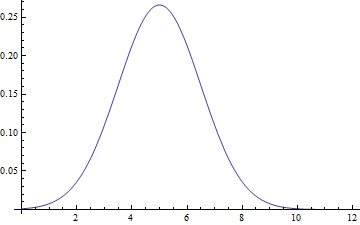
\includegraphics[width=\linewidth]{gp_1d.png}
  \caption{Univariate Gaussian}
  \label{fig:gaussian_1d}
\end{minipage}%
\begin{minipage}{.41\linewidth}
  \centering
  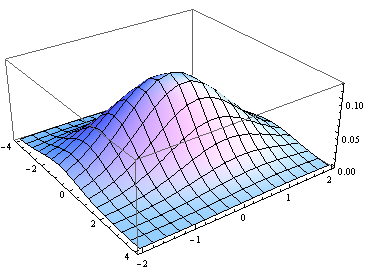
\includegraphics[width=\linewidth]{gp_2d.png}
  \caption{Multivariate Gaussian}
  \label{fig:gaussian_2d}
\end{minipage}

\label{fig:test}
\end{figure}


\subsection{Bayesian Linear Regression Model}

The traditional linear regression method is rigid in terms of learning the parameters. It gives fixed values for parameters for one observed datapoint. Therefore, for every new observed datapoint, the parameters are most likely to change. As always we only know numeric values of the parameters, it is hard to predict how much they can change for the next observed data point.  It would be effective to learn a probability distribution over the parameters rather than fixed values. Having a distribution over parameters gives us the space where the parameters can move, which is convenient to understand a stochastic process. Bayesian probability model starts with a prior distribution over parameters and changes the distribution based on observations.

Bayesian probability model is built after \textit{Bayes'} rule. It allows us to start with a prior belief on the data, which is an initial probability distribution associated with the data. Experiments generate evidences, which are used to change the prior belief, i.e. the initial distribution. The new distribution we get after incorporating the evidences is called posterior. The formulation is given below.

\subsection{Bayes' Rule}

We start with the expression of Bayes' rule. Say we have two random variables, $x$ and $y$, where $x$ is an independent variable but $y$ depends on $x$. For the sake of regression problems we assume both $x$ and $y$ as continuous variables. The probability of $x$ is given by $p(x)$, the joint probability of $x$ and $y$ is given by $p(y, x)$. We can break $p(y, x)$ in $p(y|x)p(x)$ or $p(x|y)p(y)$ (Here $p(x|y)$ cannot be written as $p(x)$ if $x$ is conditionally dependent on $y$). Therefore,

\begin{eqnarray}
p(y, x) = p(y|x)p(x) = p(x|y)p(y)\nonumber\\
p(y|x) = \frac{p(x|y)p(y)}{p(x)}
\end{eqnarray}


The term $p(x)$ is marginalized over all possible values of $y$, so we can write $p(x)$ as,

\begin{equation}
p(x) = \int_y{p(x|y)p(y)dy}
\end{equation}


Combining Eqn. \ref{reg_param} and Eqn. \ref{gauss_single_var_dist},

\begin{equation}
p(y|x) = \frac{p(x|y)p(y)}{\int_y{p(x|y)p(y)dy}}
\end{equation}

\iffalse
In case $y$ is a continuous variable,

\begin{equation}
p(y|x) = \frac{p(x|y)p(y)}{\int_y{p(x|y)p(y)dy}}
\end{equation}

\fi

\subsection{The Standard Linear Model}

We start with the assumption that $y_i$ differs from $f(\mathbf{x}_i)$ because of noise. In our discussion of regression problems in \ref{subsec:reg_prob} we had a constant parameter $\theta_0$. In this section we model that same $\theta_0$ as the noise term which, given by $\epsilon_i$, follows Gaussian i.i.d. $\mathcal{N}(0, \sigma ^2)$. Therefore the i\textsuperscript{th} observation can be written as,

\begin{eqnarray}
\label{eqn:standard_linear_model}
y_i = f(\mathbf{x}_i) + \epsilon_i \nonumber \\
y_i = \boldsymbol\theta ^T \mathbf{x}_i + \epsilon_i && \text{where $\boldsymbol\theta, \mathbf{x}_i \in \mathcal{R}^m$}
\label{gauss_noise}
\end{eqnarray}

The PDF associated with $\epsilon_i$ is,

\begin{equation}
p(\epsilon_i) = \frac{1}{\sqrt{2 \pi} \sigma} exp \Big[-\frac{\epsilon_i^2}{2 \sigma^2} \Big]
\end{equation}


Replacing $\epsilon_i$ by $(y_i - \boldsymbol\theta ^T \mathbf{x}_i)$ from Eqn. \ref{gauss_noise} ,

\begin{eqnarray}
\begin{split}
	&p(y_i - \boldsymbol\theta ^T \mathbf{x}_i) = \frac{1}{\sqrt{2 \pi} \sigma} exp \Big[-\frac{(y_i - \boldsymbol\theta ^T \mathbf{x}_i)^2}{2 \sigma^2} \Big] \\
	&p(y_i | \mathbf{x}_i, \boldsymbol\theta) = \frac{1}{\sqrt{2 \pi} \sigma} exp \Big[-\frac{(y_i - \boldsymbol\theta ^T \mathbf{x}_i)^2}{2 \sigma^2} \Big]
\end{split}
\end{eqnarray}

Thus $y_i|\boldsymbol\theta ^T, \mathbf{x}_i$ is Gaussian distributed as $y_i | \boldsymbol\theta ^T \mathbf{x}_i \sim \mathcal{N}(\boldsymbol\theta^T \mathbf{x}_i, \sigma^2)
$

Over the entire training dataset $S = \{\mathbf{x}_i, y_i\}_{i=1}^n$, as $y_i$'s are independent and identically distributed, we can write,

\begin{eqnarray}
\label{eqn:likelihood}
\begin{split}
	p(\mathbf{y} | \mathbf{X}, \boldsymbol\theta) &= \prod_{i = 1}^n p(y_i | \boldsymbol\theta ^T \mathbf{x}_i) \\
	&= \prod_{i = 1}^n \frac{1}{\sqrt{2 \pi} \sigma} exp \Big[-\frac{(y_i - \boldsymbol\theta ^T \mathbf{x}_i)^2}{2 \sigma^2} \Big]
\end{split}
\end{eqnarray}

Therefore $p(\mathbf{y} | \mathbf{X}, \boldsymbol\theta)$ is Gaussian distributed as $\mathbf{y} | \mathbf{X}, \boldsymbol\theta \sim \mathcal{N}(\boldsymbol\theta^T \mathbf{X}, \sigma^2 \mathbf{I})$

Here $\mathbf{y}_i = \{y_1, y_2, .... y_n\}$ denotes the output vector and $X = \{\mathbf{x_1}, \mathbf{x_2}, ..., \mathbf{x_n}\}$ is the matrix comprising of all the input vectors, sometimes denoted as the design matrix.



Eqn \ref{eqn:likelihood} gives us the likelihood function w.r.t. $\boldsymbol \theta$. We could take a maximum likelihood estimate here and calculate the optimal $\boldsymbol \theta$. But instead of point estimation of individual parameters, we want to calculate the distribution over $\boldsymbol \theta$ based on the observed dataset $S$. We assume a prior over $\boldsymbol \theta$ as,

\begin{eqnarray}
\label{eqn:prior}
\begin{split}
	\boldsymbol \theta \sim \mathcal{N}(\mathbf{0}, \Sigma_p)
\end{split}
\end{eqnarray}

The posterior distribution over $\boldsymbol \theta$ given $S$ would be,

\begin{eqnarray}
\begin{split}
p(\boldsymbol \theta | \mathbf{y}, \mathbf{X}) &= \frac{p(\mathbf{y} | \mathbf{X}, \boldsymbol\theta) p(\boldsymbol \theta)}{p(\mathbf{y} | \mathbf{X})} \\
&~\\
p(\boldsymbol \theta | \mathbf{y}, \mathbf{X}) & \propto p(\mathbf{y} | \mathbf{X}, \boldsymbol\theta) p(\boldsymbol \theta)
\end{split}
\end{eqnarray}

We omit the marginal likelihood term, $p(\mathbf{y} | \mathbf{X}) = \int p(\mathbf{y} | \mathbf{X}, \boldsymbol \theta)p(\boldsymbol \theta)d\boldsymbol \theta$, being a constant and this posterior over $\boldsymbol \theta$ can be shown to follow Gaussian as,

\begin{eqnarray}
\begin{split}
\boldsymbol \theta | \mathbf{y}, \mathbf{X} & \sim \mathcal{N}(\frac{1}{\sigma^2} A^{-1} \mathbf{Xy}, A^{-1})
\end{split}
\end{eqnarray}

Here $A$ is given by $\sigma^{-2} \mathbf{XX^T + \Sigma_p^{-1}}$

Now for any next unobserved data point $S_* = \{y_*, x_*\}$, we can calculate the posterior distribution over $y_*$, given $x_*$ and $S$, as below,

\begin{equation}
\label{conti_rnd_var_bayes_poster}
\begin{split}
	&p(y_* | \mathbf{x}_*, \mathbf{X}, \mathbf{y}) = \int p(y_* | \mathbf{x}_*, \boldsymbol\theta)p(\boldsymbol\theta | \mathbf{X}, \mathbf{y})d \boldsymbol\theta \\
	&y_* | \mathbf{x}_*, \mathbf{X}, \mathbf{y} \sim \mathcal{N}(\frac{1}{\sigma^2}\mathbf{x}_*^T A^{-1} \mathbf{Xy}, \mathbf{x}_*^T A^{-1} \mathbf{x}_*)
\end{split}
\end{equation}

The problem with this model is that it suffers from input dimensionality issues. If the input is of one or very few dimensions say $\mathbf{x}_i \in \mathcal{R}^2$, then the model might not be able to fit very complex non-linear functions, also if the input has a large dimension, say $\mathbf{x}_i \in \mathcal{R}^{200}$ then optimising that many parameters is cumbersome. Therefore we need a mechanism that transfers the input into another feature space of favourable dimensions.


\subsection{The Basis Function Model}
There are special functions called \textit{basis functions}, which are used to transform the input vectors into another feature space of different dimension. We can define a collection of basis functions as below,

\begin{equation}
\label{eqn:basis_function}
\begin{split}
	&\Phi(.) = \{\phi_1(.), \phi_2(.), ...,\phi_n(.)\} \mid n \in \mathcal{R}
\end{split}
\end{equation}

Say we have an input vector $\mathbf{x}_i \in \mathcal{R}^d$ as $\mathbf{x}_i = \{x_{i1}, x_{i2}, ..., x_{id}\}$, which changes when passed through the basis function. Each function from the basis function set is applied to each component of the input vector to generate $d$ numbers which are then passed to another function to generate a single number. This way we generate $\Phi(\mathbf{x}_i) \in \mathcal{R}^n$  

\begin{align}
\label{eqn:basis_function}
	\Phi(\mathbf{x}_i) =  &\Bigg\{f\bigg(\phi_1(x_{i1}), \phi_1(x_{i2}), ..., \phi_1(x_{id})\bigg), \nonumber \\ 
	 &f\bigg(\phi_2(x_{i1}), \phi_2(x_{i2}), ..., \phi_2(x_{id})\bigg), \nonumber \\ 
	 &. \nonumber \\
	 &. \nonumber \\
	 &f\bigg(\phi_n(x_{i1}), \phi_n(x_{i2}), ..., \phi_n(x_{id})\bigg)\Bigg\}
\end{align}

The standard linear model changes into,

\begin{equation}
\label{eqn:basis_function_model}
\begin{split}
	y_i = \phi(\mathbf{x}_i)^T \boldsymbol\theta + \epsilon_i
\end{split}
\end{equation}

The predictive distribution becomes,

\begin{equation}
\label{eqn:basis_function_model_predictive_distribution}
\begin{split}
	y_* | \mathbf{x}_*, \mathbf{X}, \mathbf{y} \sim \mathcal{N}(\boldsymbol\phi_*^T \Sigma_p \boldsymbol\Phi(\mathcal{K} + \sigma^2 \mathcal{I})^{-1} \mathbf{y}, \boldsymbol\phi_*^T \Sigma_p \boldsymbol\phi_* - \boldsymbol\phi_*^T \Sigma_p \boldsymbol\Phi(\mathcal{K} + \sigma^2 \mathcal{I})^{-1} \boldsymbol\Phi^T \Sigma_p \boldsymbol\phi_*)
\end{split}
\end{equation}

Here $\mathcal{K} = \boldsymbol\Phi^T \Sigma_p \boldsymbol\Phi$ and we have used some shorthands. They are $\boldsymbol\phi_* = \boldsymbol\phi_*(\mathbf{x}_*)$ and $\boldsymbol\Phi = \boldsymbol\Phi(\mathbf{X})$ \cite{gaussian_process_for_machine_learning}.

We see that some identical terms appear several times in Eqn. \ref{eqn:basis_function_model_predictive_distribution} as $\boldsymbol\Phi^T \Sigma_p \boldsymbol\Phi$, $\boldsymbol\phi_*^T \Sigma_p \boldsymbol\Phi$ and $\boldsymbol\phi_*^T \Sigma_p \boldsymbol\phi_*$. They must have been in the form $\boldsymbol\phi(\mathbf{x})^T \Sigma_p \boldsymbol\phi(\mathbf{x_*})$ where $\mathbf{x}$ and $\mathbf{x_*}$ are training and test sets. This expression has a functional form called \textit{covariance function or kernel function} as below,

\begin{equation}
\label{eqn:basis_function_model_kernel}
\begin{split}
	k(\mathbf{x}, \mathbf{x_*}) = \boldsymbol\phi(\mathbf{x})^T \Sigma_p \boldsymbol\phi(\mathbf{x_*})
\end{split}
\end{equation}

This kernel has extreme importance in practical applications. We see from Eqn. \ref{eqn:basis_function_model_predictive_distribution} that the entire expression is made up of kernel functions. We can pre-calculate the entire kernel for all possible $\mathbf{x}$ and $\mathbf{x_*}$ and then we do not need the individual input feature vectors anymore. Here, we are achieving some kind of dimensionality reduction.

Here, the problem we need to deal with is to choose the appropriate amount of basis functions, their location centres, their width etc. As the kernel function is built with the inner product of input vectors elevated to the basis feature space, these parameters play an important role and if not chosen carefully they might not reflect the proper covariance between the given input. The most obvious drawback is the correlation between the inputs falls of quickly when they move far away from the basis function centres. We need an infinite amount of basis functions to reflect the true covariance between the inputs. This discussion is out of scope for this text. In the next section, we will see how we can build an efficient kernel function that does not have to deal with the setting of these basis function parameters, rather it directly relates the given inputs and instead of trying to get the distribution over parameters, it directly calculates the posterior over the function $f\mathbf(x)$. In other words, instead of calculating posterior over $\mathbf(X)^T \boldsymbol\theta$ or $\boldsymbol\phi \mathbf(X)^T \boldsymbol\theta$, we directly calculate the posterior over $f\mathbf(x)$. It frees us from dealing with $\boldsymbol \theta$ or $\boldsymbol \phi$. Here, comes the idea of \textit{Gaussian Process}.

\subsection{Gaussian Process}

Gaussian process \cite{gaussian_process_for_machine_learning} is a mathematical framework that does not try to learn a finite set of parameters. It models the output as a function of covariances between the input data points. It tries to learn the function that gives that output over any input. In other words it tries to learn the distribution over the functions. As it expresses the function in terms of input covariances, it does not care about dimensions of input once covariances are calculated, thus it truly represents a non parametric multivariate Gaussian framework. This representation is known as Gaussian process.

In our example of rainfall prediction, we consider $x_i \in \mathcal{R}$ to be summer temperature. Here the independent random variable $x_i$ is single dimensional. If we consider spring temperature also for that particular year then $\mathbf{x}_i = \{x_i, x_j\} \in \mathcal{R}^2$ becomes two dimensional. No matter how many different temperatures we consider, $\mathbf{x}_i \in \mathcal{R}^d$ remains a finite dimensional vector. Gaussian process helps in building a framework that actually allows us to fit any number of dimensions in. We do not have to fix $d$ beforehand. Therefore we can make $\mathbf{x}_i$ represent various different temperatures at different months, weeks, days, hours and so forth.

Here, we show set of observations $\mathcal{X}$ on $X$- axis i.e. $\mathbf{x}_i$ values. As we can fit infinite number of points on $X$- axis, we can represent infinite amount of observations on it. If $\mathcal{X}$ is a set of three observations, we show three points on $X$-axis.

To represent the regression problem here, we have,

\begin{equation}
y_i = f(\mathbf{x}_i) + \epsilon_i
\label{reg_sym_noise}
\end{equation}

$\epsilon_i \sim (0, \sigma^2))$ is the standard Gaussian noise.

Without considering any parameter set, we try to learn the function $f$. We treat $f$ as a dependent random variable on $\mathbf{x}_i$. A continuous function can represent an infinite number of points on it. Therefore, $f$ can fit an infinite number of $\mathbf{x}_i$, where $i = 0, 1, ... \infty$. Thus, Gaussian process gives us an infinite dimensional multivariate Gaussian distribution or a distribution over functions.

\begin{figure}[ht!]
     \begin{center}
%
        \subfigure[Prior with zero mean]{%
            \label{fig:gp_first}
            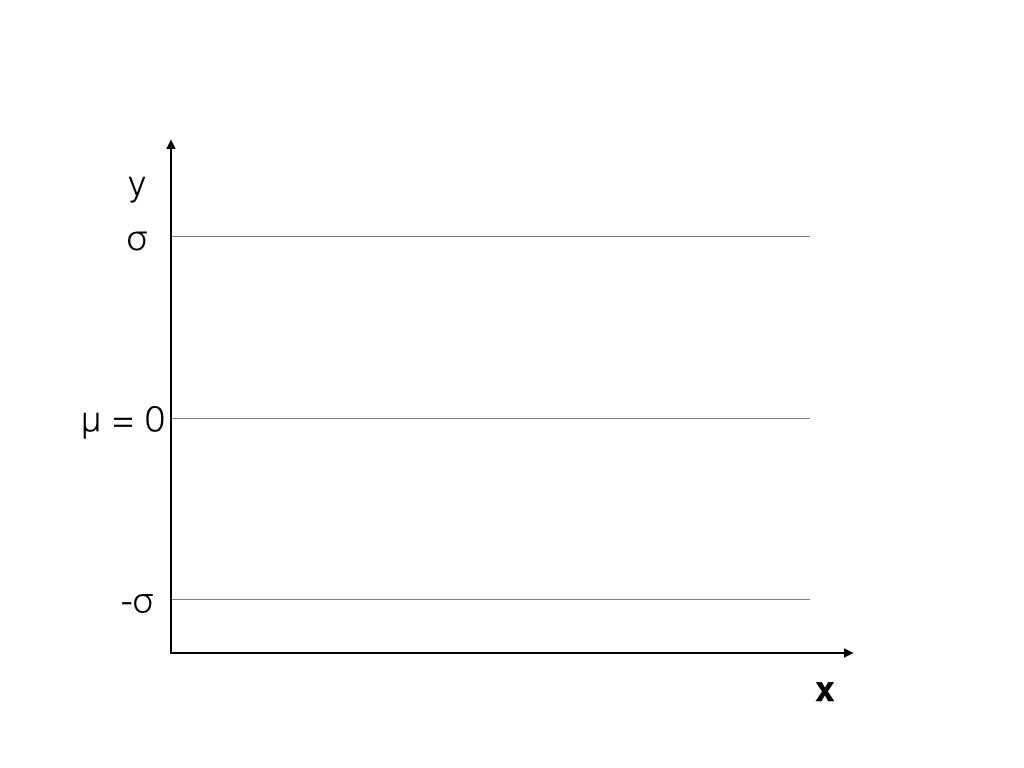
\includegraphics[width=0.5\textwidth]{figures/GP_1.png}
        }%
        \subfigure[Posterior with one evidence]{%
           \label{fig:gp_second}
           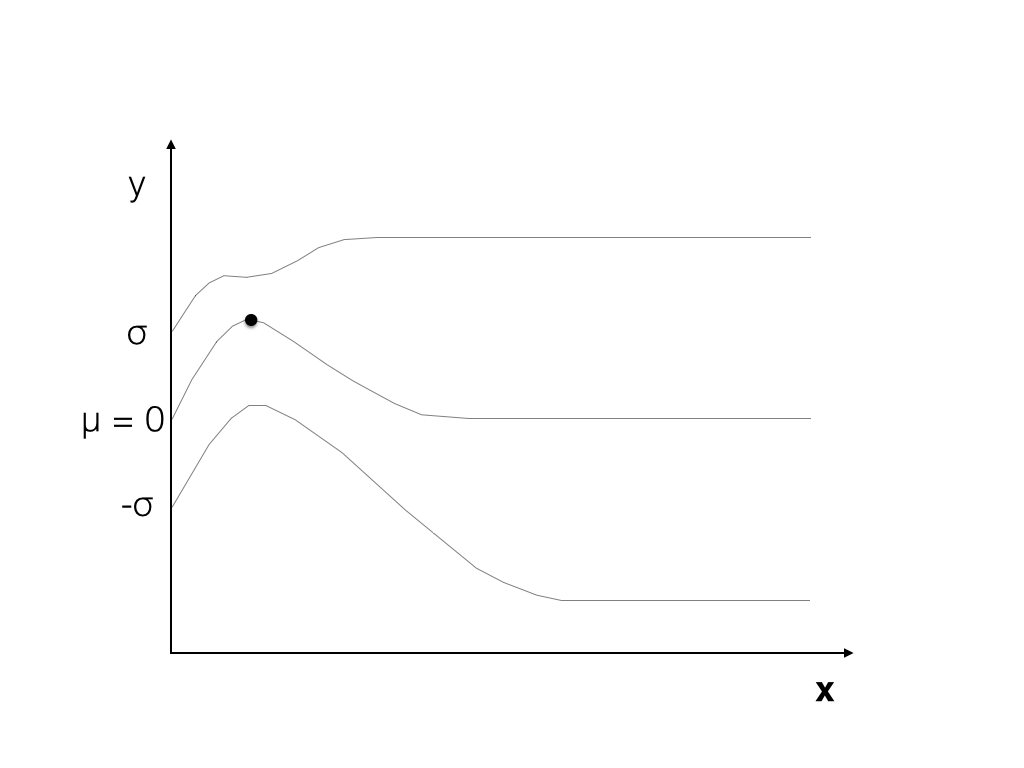
\includegraphics[width=0.5\textwidth]{figures/GP_2.png}
        }\\ %  ------- End of the first row ----------------------%
        \subfigure[More evidences]{%
            \label{fig:gp_third}
            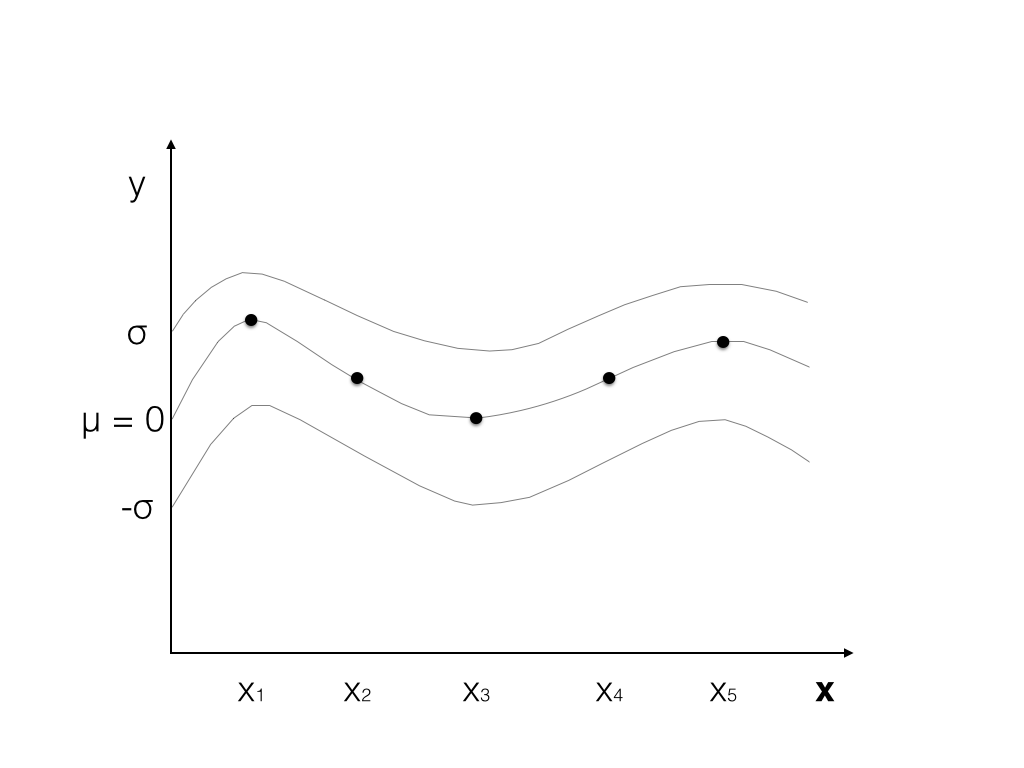
\includegraphics[width=0.5\textwidth]{figures/GP_3.png}
        }%
        \subfigure[Learned function with entire training set]{%
            \label{fig:gp_fourth}
            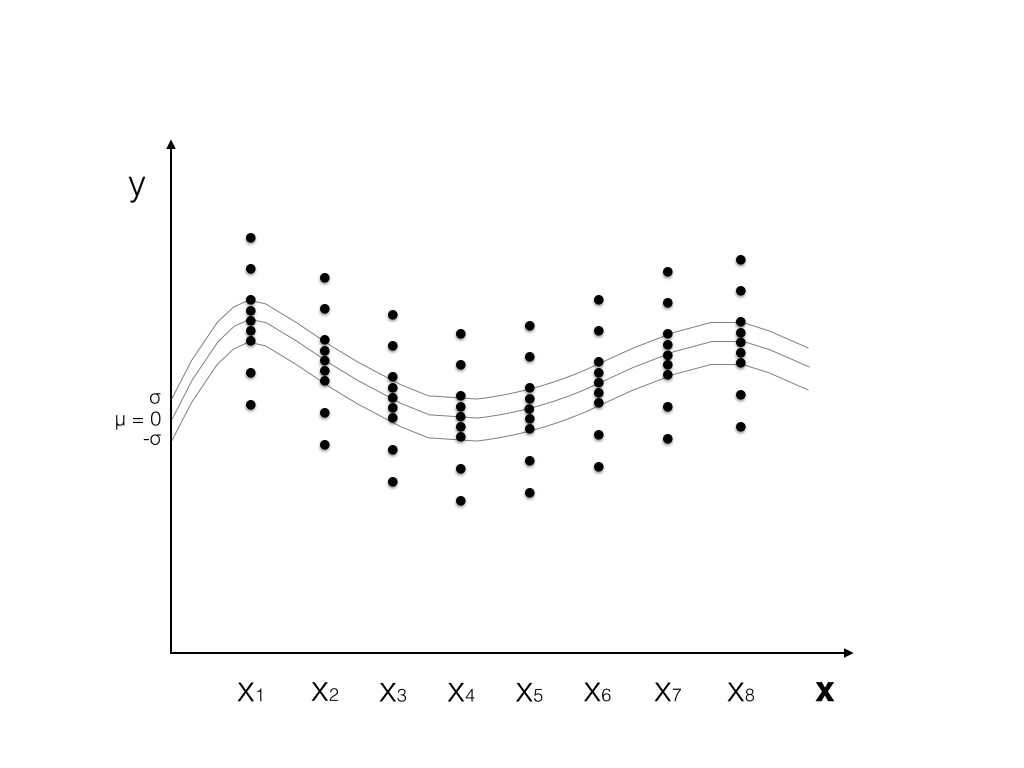
\includegraphics[width=0.5\textwidth]{figures/GP_4.png}
        }%
%
    \end{center}
    \caption{%
        Visual representation of Gaussian process.
     }%
   \label{fig:gaussian_process}
\end{figure}

\iffalse

\begin{figure}[h!]
\centering
\begin{minipage}{.5\linewidth}
  \centering
  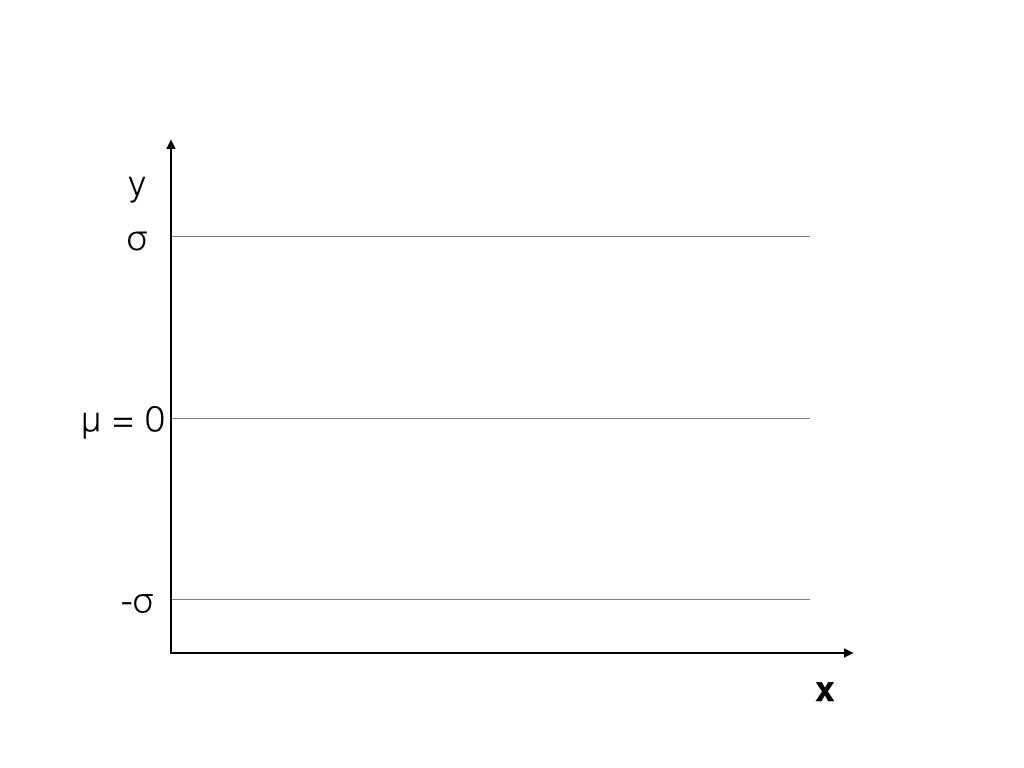
\includegraphics[width=\linewidth]{figures/GP_1.png}
  \caption{Prior with zero mean}
  \label{fig:sub1}
\end{minipage}%
\begin{minipage}{.5\linewidth}
  \centering
  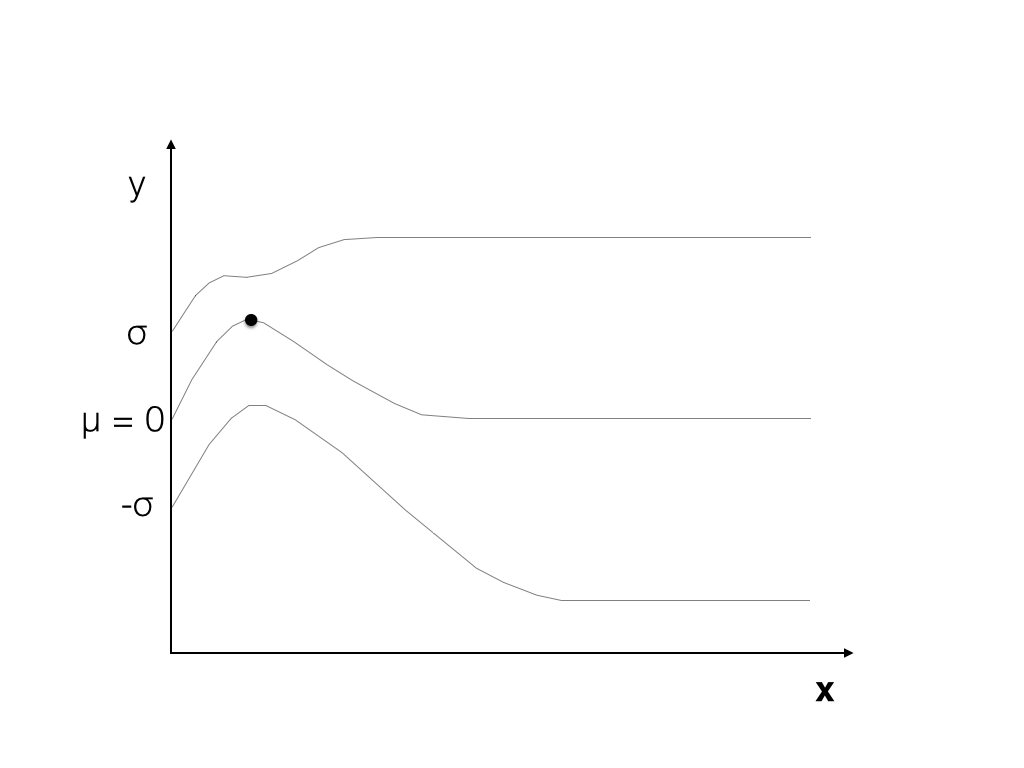
\includegraphics[width=\linewidth]{figures/GP_2.png}
  \caption{Posterior with one evidence}
  \label{fig:sub2}
\end{minipage}

\begin{minipage}{.5\linewidth}
  \centering
  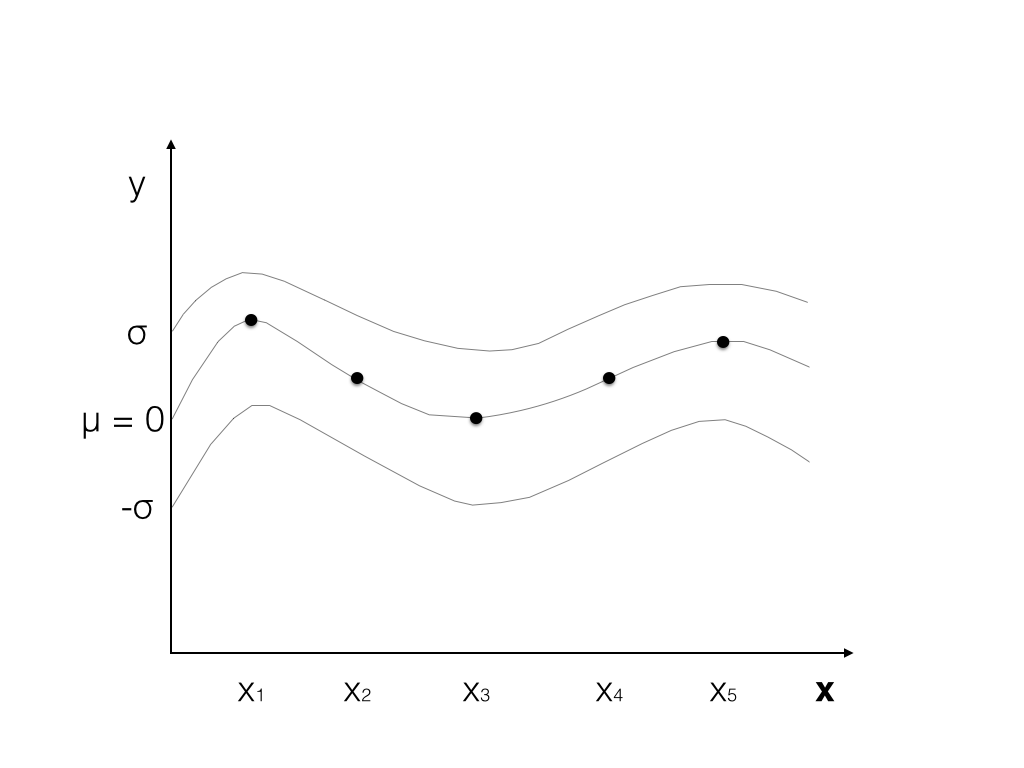
\includegraphics[width=\linewidth]{figures/GP_3.png}
  \caption{More evidences}
  \label{fig:sub1}
\end{minipage}%
\begin{minipage}{.5\linewidth}
  \centering
  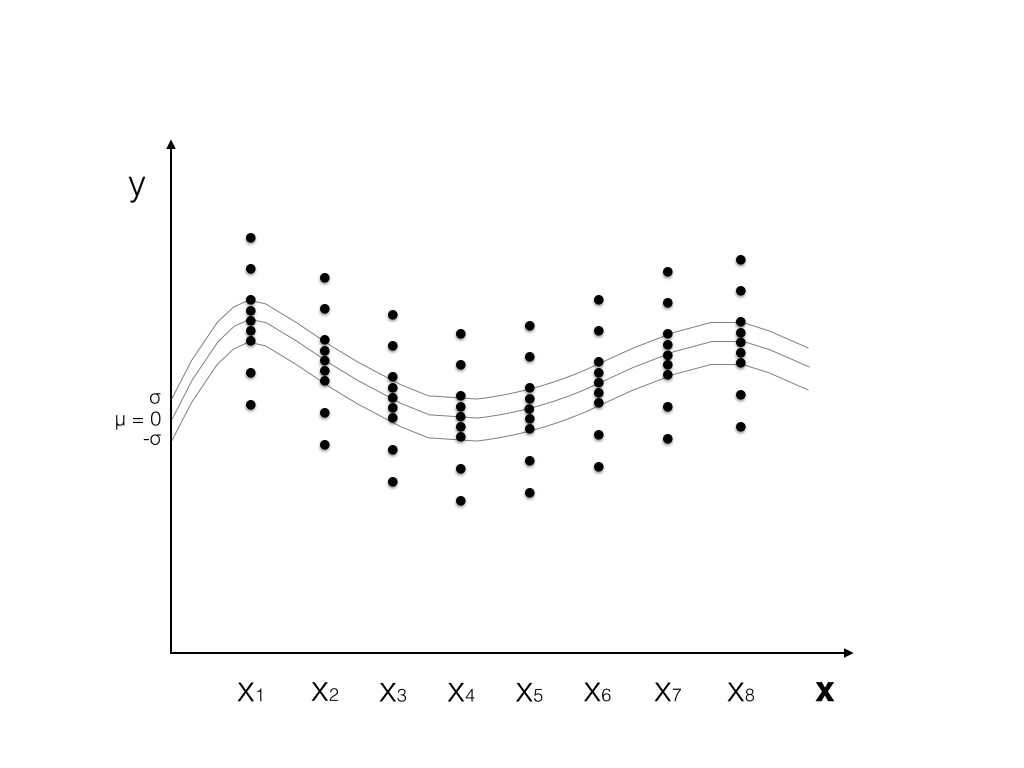
\includegraphics[width=\linewidth]{figures/GP_4.png}
  \caption{Learned function with entire training set}
  \label{fig:sub2}
\end{minipage}

\label{fig:test}
\end{figure}

\fi

Say, $\mathcal{F} = \{f_1, f_2, ..., f_n, f_{n+1}, ... \infty\}$ is a set of functions that can operate over $\mathbf{x}_i$. Any function $f$ over an $x$ can take any form like $f(x) = (x + 2)$ or $f(x) = x^2$ or $f(x) = \exp(\sin(x)^5)$, as long as $f(x) \in \mathcal{R}$. From this infinite set $\mathcal{F}$, we need to find the proper $f$ that truly represents $y$ i.e. truly fits the data.

To differentiate a function from a regular random variable we denote a function $f$ as $f(.)$ from now on. We start with a prior distribution over $\mathcal{F}$, given by,

\begin{equation}
f(.) \sim (m(.), k(.,.))
\end{equation}

Figure \ref{fig:gaussian_process} presents a visual representation of Gaussian process. The prior is shown in \ref{fig:gp_first} with zero mean. Before getting evidences, the prior distribution has uniform confidence interval around the mean for the entire input space. After getting one evidence point the space around that point shrinked as shown in \ref{fig:gp_second}. We exclude all the functions that do not pass through our evidence point. The mean function has to pass through that point, therefore it is shifted and the confidence interval also narrowed down accordingly. \ref{fig:gp_third} shows the same effect for more evidence points. \ref{fig:gp_fourth} finally shows the shape of the posterior function when we have enough evidences.

As we are operating on a distribution over functions, the mean $m(.)$ and covariance $k(.,.)$ are also functions. The domain of $f(.)$ is a vector $\mathbf{x}_i \in \mathcal{R}^d$ where $d \to \infty$. $m(.)$ is the mean function which gives the mean of any input $\mathbf{x}_k \in \mathcal{X}$ as $m(\mathbf{x}_k) = \mu_{\mathbf{x}_k}$ and it generates a mean vector over $\mathcal{X}$ as,

$$
m(\mathcal{X}) = \{m(\mathbf{x}_k) \mid k = 0, 1, 2, ...\} = \{\mu_{\mathbf{x}_k} \mid k = 0, 1, 2, ...\} 
$$

$k(.,.)$ takes two random vectors, $\mathbf{x}_k$ and $\mathbf{x}_l$ from $\mathcal{X}$ and gives the covariance between them as,

$$
k(\mathbf{x}_k, \mathbf{x}_l) = Covariance(\mathbf{x}_k, \mathbf{x}_l)
$$

$k(.,.)$ is also called the Kernel function as discussed before.

To represent the multivariate distribution over functions operating over any finite subset $\mathcal{X}_m \in \mathcal{X}$ we can write in matrix form as,

$$
\begin{pmatrix}
f(\mathbf{x}_1) \\
f(\mathbf{x}_2) \\
\vdots \\
f(\mathbf{x}_m)
\end{pmatrix}
\sim \mathcal{N} \left(%
\begin{pmatrix}
m(\mathbf{x}_1) \\
m(\mathbf{x}_2) \\
\vdots \\
m(\mathbf{x}_m)
\end{pmatrix}
,%
\begin{pmatrix}
k(\mathbf{x}_1, \mathbf{x}_1) k(\mathbf{x}_1, \mathbf{x}_2) \hdots k(\mathbf{x}_1, \mathbf{x}_m) \\
k(\mathbf{x}_2, \mathbf{x}_1) k(\mathbf{x}_2, \mathbf{x}_2) \hdots k(\mathbf{x}_2, \mathbf{x}_m) \\
\vdots \\
k(\mathbf{x}_m, \mathbf{x}_1) k(\mathbf{x}_m, \mathbf{x}_2) \hdots k(\mathbf{x}_m, \mathbf{x}_m) 
\end{pmatrix}\right)
$$

Here, the left hand side represents the output vector, the right hand side represents the multivariate Gaussian distribution over functions with a mean vector and a covariance matrix. Which can be written as,

\begin{equation}
f(\mathcal{X}_m) \sim \mathcal{N} (m(\mathcal{X}_m), K(\mathcal{X}_m))
\label{gauss_proc_multi_var_sym}
\end{equation}

We see how easy Gaussian process is to customize, any time we can extract a finite subset out of the infinite distribution.

To simplify the calculation, we start with a zero mean prior as,

\begin{equation}
f(.) \sim \mathcal{N} (0, k(.,.))
\label{gauss_proc_func_0_mean_sym}
\end{equation}

Combining Eqn. \ref{gauss_proc_multi_var_sym} and Eqn. \ref{gauss_proc_func_0_mean_sym} we get,

\begin{equation}
f(\mathcal{X}_m) \sim \mathcal{N} (0, K(\mathcal{X}_m))
\label{eq:gp_training}
\end{equation}

We take $\mathcal{X}_m$ as training set, so we have observed $\mathbf{y}_m$. Say we have another finite subset $\mathcal{X}_m^*$, which is the test set. We need to predict outputs $\mathbf{y}_m^*$ for $\mathcal{X}_m^*$. Both the subsets came from the same infinite Gaussian distribution. So for $\mathcal{X}_m^*$ we write,

\begin{equation}
f(\mathcal{X}_m^*) \sim \mathcal{N} (0, K(\mathcal{X}_m^*))
\label{eq:gp_test}
\end{equation}

We combine Eqn. \ref{eq:gp_training} and Eqn. \ref{eq:gp_test} together as,

\begin{equation}
\begin{pmatrix}
f(\mathcal{X}_m) \\
f(\mathcal{X}_m^*)
\end{pmatrix}
\sim \mathcal{N} \left( %
0, %
\begin{pmatrix}
K(\mathcal{X}_m, \mathcal{X}_m) & K(\mathcal{X}_m, \mathcal{X}_m^*) \\
K(\mathcal{X}_m^*, \mathcal{X}_m) & K(\mathcal{X}_m^*, \mathcal{X}_m^*)
\end{pmatrix}\right)
\end{equation}

We also have noise vectors $\mathbf{\varepsilon} \in \mathcal{R}^m$ and $\mathbf{\varepsilon^*} \in \mathcal{R}^m$. We get the distribution over $\mathbf{y}$ by adding noise to the distribution over $f(.)$. Addition of multiple Gaussians remains Gaussian, so we can write,

\begin{eqnarray}
\begin{pmatrix}
\mathbf{y}_m \\
\mathbf{y}_m^*
\end{pmatrix}
= %
\begin{pmatrix}
f(\mathcal{X}_m) \\
f(\mathcal{X}_m^*)
\end{pmatrix}
+%
\begin{pmatrix}
\mathbf{\varepsilon} \\
\mathbf{\varepsilon^*}
\end{pmatrix}
\sim \mathcal{N} \left( %
0, %
\begin{pmatrix}
K(\mathcal{X}_m, \mathcal{X}_m) + \sigma^2 \mathbf{I} & K(\mathcal{X}_m, \mathcal{X}_m^*) \\
K(\mathcal{X}_m^*, \mathcal{X}_m) & K(\mathcal{X}_m^*, \mathcal{X}_m^*) + \sigma^2 \mathbf{I}
\end{pmatrix}\right)
\end{eqnarray}

Using Bayesian posterior calculation it can be shown that,

\begin{equation}
\mathbf{y_m}^* | \mathbf{y_m}, \mathcal{X}_m, \mathcal{X}_m^* \sim (\mu^*, \Sigma^*)
\end{equation}

This is the function represented by Figure 4.

where,

\begin{equation}
\mu^* = K(\mathcal{X}_m^*, \mathcal{X}_m)(K(\mathcal{X}_m, \mathcal{X}_m) + \sigma^2 \mathbf{I})^{-1}\mathbf{y_m}
\label{gauss_poster_mean}
\end{equation}

and,

\begin{equation}
\Sigma^* = K(\mathcal{X}_m^*, \mathcal{X}_m^*) + \sigma^2 \mathbf{I} - K(\mathcal{X}_m^*, \mathcal{X}_m)(K(\mathcal{X}_m, \mathcal{X}_m) + \sigma^2 \mathbf{I})^{-1} K(\mathcal{X}_m, \mathcal{X}_m^*)
\label{gauss_poster_var}
\end{equation}

\begin{figure*}[htb] 
\centering
 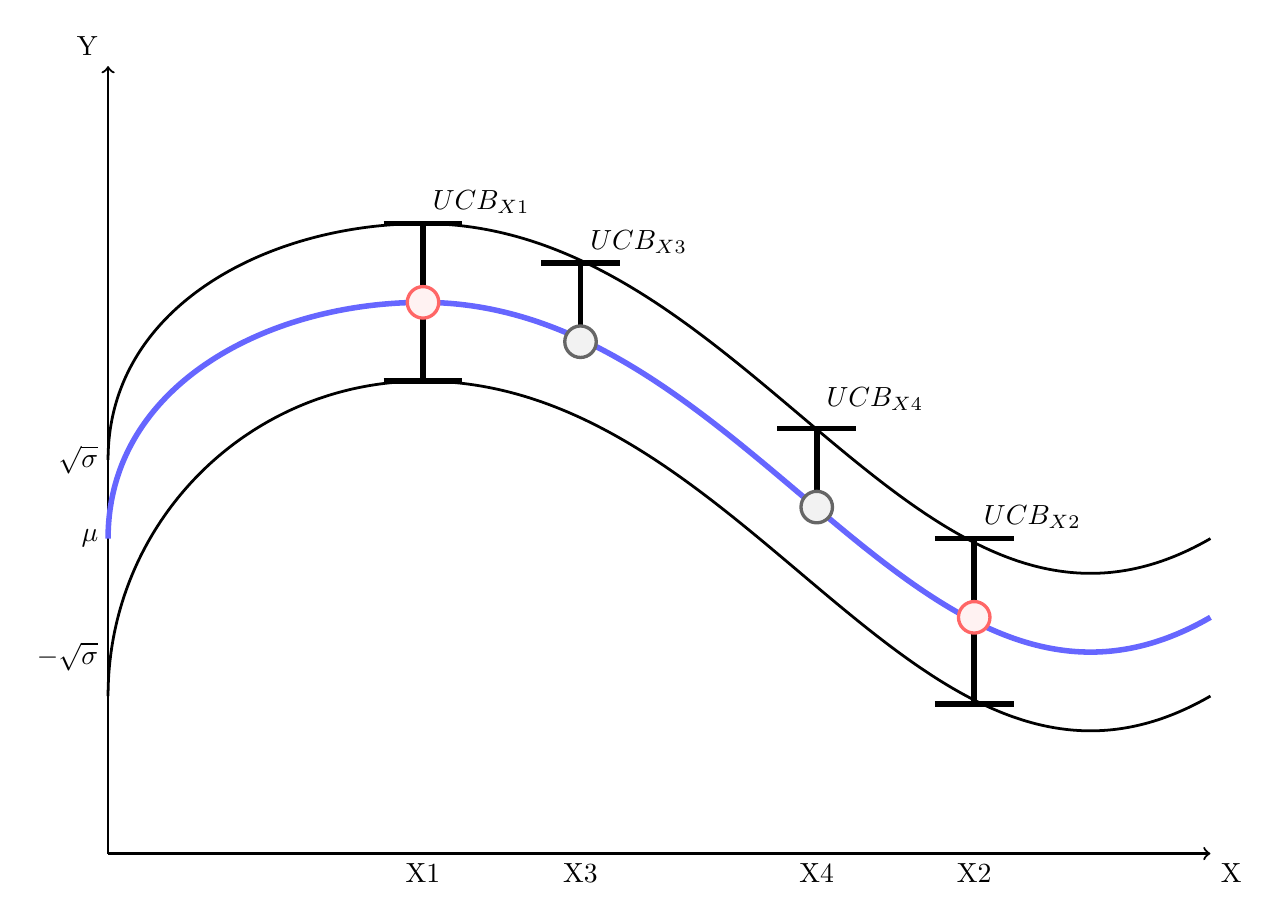
\begin{tikzpicture}


% Draw Axis

\draw[thick,->] (0,0) -- (14,0) node[anchor=north west]{X};
\draw[thick,->] (0,0) -- (0,10) node[anchor=south east]{Y};

% Draw Mean function
\draw[color=blue!60, line width=2pt] (0,4) to [out=90, in=180] (4,7)
to [out=0, in=210] (14,3);

% Draw Lower Bound (-var) function

\draw[line width=1pt] (0,2) to [out=90, in=180] (4,6)
to [out=0, in=210] (14,2);

% Draw Upper Bound (+var) function

\draw[line width=1pt] (0,5) to [out=90, in=180] (4,8)
to [out=0, in=210] (14,4);

% Draw Confidence Interval for X1

\draw[line width = 2pt] (4,6) -- (4,8);

\draw[line width = 2pt] (3.5,6) -- (4.5,6);

\draw[line width = 2pt] (3.5,8) -- (4.5,8);

% Draw X1

\filldraw[color=red!60, fill=red!5, very thick] (4,7) circle (0.2cm);

% Draw Confidence Interval for X2

\draw[line width = 2pt] (11,1.9) -- (11,4);

\draw[line width = 2pt] (10.5,1.9) -- (11.5,1.9);

\draw[line width = 2pt] (10.5,4) -- (11.5,4);

% Draw X4

\filldraw[color=red!60, fill=red!5, very thick] (11,3) circle (0.2cm);

% Draw dashed Confidence Interval for X3

\draw[line width = 2pt] (6,6.5) -- (6,7.5);

\draw[line width = 2pt] (5.5,7.5) -- (6.5,7.5);

% Draw X3

\filldraw[color=black!60, fill=black!5, very thick] (6,6.5) circle (0.2cm);

% Draw dashed Confidence Interval for X4

\draw[line width = 2pt] (9,4.4) -- (9,5.4);

\draw[line width = 2pt] (8.5,5.4) -- (9.5,5.4);

% Draw X4

\filldraw[color=black!60, fill=black!5, very thick] (9,4.4) circle (0.2cm);

% Draw Labels on X-Axis

\node [below] at (4,0) {X1};

\node [below] at (11,0) {X2};

\node [below] at (6,0) {X3};

\node [below] at (9,0) {X4};

% Draw Labels on Y-Axis

\node [left] at (0,4) {$\mu$};

\node [left] at (0,2.5) {$-\sqrt{\sigma}$};

\node [left] at (0,5) {$\sqrt{\sigma}$};

% Draw UCB Labels

\node [above right] at (4,8) {$UCB_{X1}$};

\node [above right] at (11,4) {$UCB_{X2}$};

\node [above right] at (6,7.5) {$UCB_{X3}$};

\node [above right] at (9,5.5) {$UCB_{X4}$};

\end{tikzpicture}
\caption{Gaussian process upper confidence bound}
\label{fig:gp_ucb}
\end{figure*}

\subsection{Applying Gaussian Process to Bandit Problems}

We ended \ref{sec:UCB} by mentioning that upper confidence bound works well in finite action spaces. Gaussian process helps us is determining upper confidence bound in infinitely large action spaces, where estimating mean for each action distribution is practically impossible. We represent the actions $A$ as our input space as before and we want to learn a function that gives mean rewards $\mu_{a_i}$ for each $a_i$. Theoretically the more $a_i$s we explore, the closer we get to the actual reward function. But in real life experiments it is not always possible to try all or nearly all the actions from a very large action space.





By carefully observing how the posterior of the reward function changes given the observations so far and then choosing the next action, we can nearly estimate the actual reward function very quickly. This requires some optimisation over selection of actions which is beyond the scope of this discussion. Also the more we select each action, by the \textit{law of large numbers}, the closer we go to the actual mean reward associated with that action. Figure \ref{fig:gp_ucb} shows the upper confidence bound as the positive standard deviation (square root of variance) added to mean. $UCB_{X1}$, $UCB_{X2}$, $UCB_{X3}$ and $UCB_{X4}$ represent the upper confidence bounds of data points $X1$, $X2$, $X3$ and $X4$ respectively.

Next we will see how we modelled our system based on these discussion.



\section{System description}

Our system has a collection of $25000$ images. The system \cite{re_qlir} shows a random set of a few images to the user and collects relevance feedback on each shown image. If the user does not give feedback to any of the shown images, the system assumes zero feedback on all of them and proceeds accordingly. The indices of the shown images are taken to be the inputs and the collected relevance feedbacks as outputs, where these inputs and outputs together form the collected evidences. These evidences are then fed to the Gaussian process framework. For the rest of the images which are not shown so far, the Gaussian process calculates the mean and variance and then the UCB value as discussed before. The image with the largest UCB value is picked by the system.

Bandit algorithms are designed to make one prediction at a time and each prediction takes the immediate reward received by the previous prediction into account. To select a set of images at each iteration, we needed to run the algorithm a few times. But, as before showing an image to the user, we do not have the relevance score for it ready, we use pseudo feedback to pick the next image. This pseudo feedback is nothing but the posterior mean for the corresponding image. Once we select the desired number of images, we show them to the user, receive relevance feedback on them, replace the pseudo feedbacks with the actual feedbacks given by our user \cite{imse}. This way we nullify the long term effect of pseudo feedbacks in our system.

We run Gaussian process as many times as the number of images to be shown per iteration to get the next set of images.

We have discussed how our system uses relevance feedback from users as immediate rewards in each step to show more and more relevant images to the users in forthcoming iterations. But if it exploits too much, it could get stuck into a context trap. We needed to have a proper balance in the amount of exploration and exploitation to avoid the context trap \cite{dir_expl_search, cbir_multinomial_rel_feed, iter_rel_feed}. Faceted search \cite{faceted_search_1, faceted_search_2} tried to avoid context trap using global image features but as global features are huge in number, the user had to traverse a vast area of the information space \cite{info_space} leading to a cognitively demanding task. Also, initially when we have a small amount of evidences, Gaussian process can produce a very wide variance for some images far away from shown images as shown in Figure \ref{fig:gaussian_process}(b). This can lead to a high UCB value for not so relevant images. This way the system will explore too much unnecessarily. To tackle this problem we introduce a term \textit{exploration rate} which is nothing but a multiplying factor ($<1$) that reduces the effective variance.

\subsection{Offline step}

We needed to process the images before starting the actual experiments. Therefore we broke the operation down into two parts as described below. These steps are performed only once before the actual experiment starts.

\subsubsection{Feature extraction}

We used MIRFLICKR 25000 \cite{mirflickr} image set for the experiment. We are considering only colour feature for this study. We represent each image as a 512 dimensional vector \cite{imse}. We used \textit{openCV} library to extract "rgb histogram" of each of the images and created an array of the histogram bins. Then, we normalised this array from $0$ to $1$. This array is the feature vector of the image concerned. We consider only colour feature.

\subsubsection{The Kernel}

We use "Cityblock" or "Manhattan" distance to calculate pairwise distance between two images, to feature vectors precisely. Manhattan distance of two vectors is nothing but the sum of absolute values of the element wise distances of the vectors given. If $\mathbf{x}$ and $\mathbf{y}$ are two vectors of equal length then $L$, their Manhattan distance would be $d_{Manhattan}(\mathbf{x}, \mathbf{y}) = \sum \limits_l^L |x_l - y_l|$, where $x_l$ and $y_l$ are $l$th values of the two vectors respectively. The distance is normalized by the number of dimensions i.e. 512. Therefore the number of dimensions are used as the length scale hyperparameter for the kernel. For any two images $x_i$ and $x_j$, the kernel function is,

\begin{equation}
K(\mathbf{x}_i, \mathbf{x}_j) = \sum_{l = 1}^{512}\frac{(|x_i^l - x_j^l|)} {512}
\end{equation}

Here $x_i^l$ and $x_j^l$ represent the $l$th dimensional value in the corresponding feature vectors of images $x_i$ and $x_j$ respectively.


We calculate all the pairwise distances among the images and build a $(25000 \times 25000)$ distance matrix. This matrix serves as the entire co-variance matrix.

\subsubsection{Clustering images}

As we have a huge number of images, calculating UCB values for nearly all of them would be severely time consuming in each iteration. We can avoid doing so for very distant images. We apply K-means \cite{k_means} clustering algorithm to cluster images as mentioned by \cite{hierarchical_gp}. Each cluster centroid is the average of all the feature vectors allocated to it. To select an image, we first calculate the UCB values for the cluster centroids and select the nearest one. Then we calculate UCB values for images only in that cluster and find out the nearest image.

\subsection{The online step} \label{experiment_1}

The user is presented a set of random images. He finds one or more suitable images inside that set (there might not be one, we will discuss that later) and provides relevance feedback as shown in Figure \ref{system_diagram_1}. The system collects the shown image set with the given relevance feedback and sends the indices of the shown images and the set of feedbacks along with the cluster centroids to the Gaussian process. This is the first run of the Gaussian process. The process returns the nearest cluster to the shown images. Now the system sends the images assigned to the selected cluster along with the same set of shown images with their received feedback again into the Gaussian process as the second run. The process returns the nearest image to show to the user. This two phase procedure is run with proper inclusion of pseudo feedback discussed earlier to come up with the next set of suitable images until the user gets the desired image.


\begin{figure}[h!]
  \centering
    \includegraphics[width=1.0\textwidth]{figures/Imse_System_Diagram}
    \caption{System diagram with hierarchical GP}
    \label{system_diagram_1}
\end{figure}

Say, upto $t$ iterations, we showed $X_t = \{x_1, x_2, ..., x_t\}$ images and received relevance feedback $Y_t = \{y_1, y_2, ..., y_t\}$.

According to Eqn. \ref{gauss_poster_mean}, for the rest of the images, the posterior mean function would be,

\begin{equation}
\mu(x) = K(x, X_t)[K(X_t, X_t) + \sigma_{noise}^2I]^{-1}Y_t
\end{equation}

and, according to Eqn. \ref{gauss_poster_var}, the posterior co-variance function would be,

\begin{equation}
\sigma^2(x) = [K(x, x) + \sigma_{noise}^2I] - K(x, X_t)[K(X_t, X_t) + \sigma_{noise}^2I]^{-1}K(x, X_t)^T
\end{equation}

At $t+1$ iteration, image $x_{t+1}$ would be selected, satisfying,

\begin{equation}
x_{t+1} = argmax_x(\mu(x) + \beta\sqrt{\sigma^2(x)})
\end{equation}

We saw in our discussion of Gaussian process that after observing a significant amount of datapoints, the posterior variance becomes very small. Therefore, the UCB value merely reflects the posterior mean, leading to an almost zero exploration. To keep the exploration alive, $\beta$ is introduced, which is a fraction that grows with discrete time or iterations. At any iteration $t$, $\beta = \sqrt{\log t}$.

\subsection{The interface}

Our objective was to build a useful and easy to use interface which supports query less exploratory image search \cite{pichunter, PicSOM, iter_rel_feed} while keeping the cognitive load of the user as low as possible. We went for a simple and clean interface, intuitive to understand, supporting visual guidance and feedback and with minimum textual instructions on screen. The main idea behind the design of the interface was to make it support query less exploratory image search while accommodating feedback given by the users. The user navigates through images and gives ratings to images indicating how close they are to what the user is searching for. According to Cox et. al. \cite{pichunter} this type of interfaces are easy to use. The interface shows images in a grid like structure as shown in Figure \ref{fig:sample_interface}. The user has to drag a sliding bar shown on-mouse-over each image to provide the feedback. The user can give feedback to any number of images and then click 'Next' at the top right corner. The display is refreshed with the next set of images.

\begin{figure}[h!]
  \centering
    \includegraphics[width=0.90\textwidth,height=6cm]{figures/Seashore_4.png}
    \caption{The interface}
    \label{fig:sample_interface}
\end{figure}

\section{Experiments}

We assign search tasks to users, say to find a "red rose". Each experiment consists of a single task. The user is asked to find out a suitable image for the given task. Based on the nature of the task we sometime show sample images but not always. The aim of these experiments were to study 1) how good exploration-exploitation strategy performs compared to mere exploitative method, 2) applicability of exploration based search in different kinds of tasks with varying abstractness. Tasks are organised into categories as described below.

\subsection{Tasks and Task-Categories}

 We could think of three different task types in terms of abstractness of the given task. Some tasks are very particular in nature. While having such a task, the user has to find out that very image described by the task. No other similar image can terminate the search. For example if the user has to find the Eiffel Tower or the Statue of Liberty etc. Some tasks are a bit generic than the ones mentioned before. For example if the user has to find out an image of sunset or seashore. They are not specific objects but are combination of objects in different colours and shapes with some similarities. There are a third kind of tasks which are very abstract in nature. Say the user has to find out happiness. We cannot attach any specific object to it. It is a state of mind and a matter of perception. For an user a picture of a happy face can be happiness, for another user a rainbow can be happiness or children in a playground can be happiness. We followed Pichunter \cite{pichunter} to design three different categories of tasks for users as follows,

\begin{enumerate}
  \item Target search - Look for a specific image
  \item Category search - Look for a category
  \item Open ended search - Find a story, i.e. a set of images that gives a theme for an essay or an article
\end{enumerate}

\textit{Target search} was the most restrictive search, requiring the user to find out an image say of a blue car.

\textit{Category search} was a bit broader, say to find a cat.

\textit{Open ended search} was the most broad one where the user was given no specific image to search for but a topic or theme like a visit to paris, out of which several images could be listed for an article on the same.

Each of these searches had three separate sub tasks as follows,

\textbf{for Target search}

\begin{enumerate}
  \item Red rose
  \item City by night
  \item Tall building
\end{enumerate}

\textbf{for Category search}

\begin{enumerate}
  \item Fruit
  \item Sunset
  \item Seashore
\end{enumerate}

\textbf{for Open ended search}

\begin{enumerate}
  \item A trip to africa
  \item Architecture
  \item Gardening
\end{enumerate}

Therefore, we had nine separate search tasks altogether. An user had to perform all these tasks but the order was different for each user. We took a set of the nine tasks, prepared twenty different random permutations out of them and assigned one to each user.

\subsection{Participants and task allocation}

We recruited twenty postgraduate students from university as participants. Before the actual experiments, we provided a short training to them on the search interface. Each participant was instructed to finish a search task whenever they had felt done i.e. "red rose" is found or enough images gathered for writing an essay on "gardening". The participants were allowed to go for 25 iterations maximum even if they had not found suitable images.

As mentioned earlier, the goal of this study was to find out how well our algorithm performs over pure exploitation. For the sake of completeness, we also had one algorithm for random selection of images. This algorithm is the simplest, which does nothing but selects images randomly without taking relevance feedback into consideration. Therefore, we compared three different algorithms, Gaussian process upper confidence bound(GPUCB), Exploitation(EXPLOIT) and Random(RAND).

For each participant, the three subtask for each major task (target, category or open-ended) were a permutation of GPUCB, EXPLOIT and RAND. We also assigned random permutations of target, category and open-ended searches to different participants, so that they could not infer what is coming next.

The participants did not know what algorithm had been used behind each task they performed.

In total we had 20 participants, each running a separate experiment out of a randomly permuted set of 9 search tasks. We recorded the following parameters,

\begin{enumerate}
	\item The username
	\item The task type
	\item The task name
	\item The algorithm running behind the task
	\item The start time
	\item The indices of the images shown per iteration
	\item The numeric value of the feedback collected for each image
	\item The running time of an iteration
	\item The end time
\end{enumerate}

\section{Results}

We studied two things, firstly, how quickly i.e. in how many iterations, GPUCB can finish compared two the EXPLOIT and RAND. Secondly, how many images get positive feedback on average in GPUCB compared to EXPLOIT and RAND \cite{explor_exploit_img_ret}. This comparison measures how many more relevant images GPUCB produces compared to the other two over an entire experiment, i.e. the overall effectiveness of GPUCB.

\begin{figure}[h!]
  \centering
    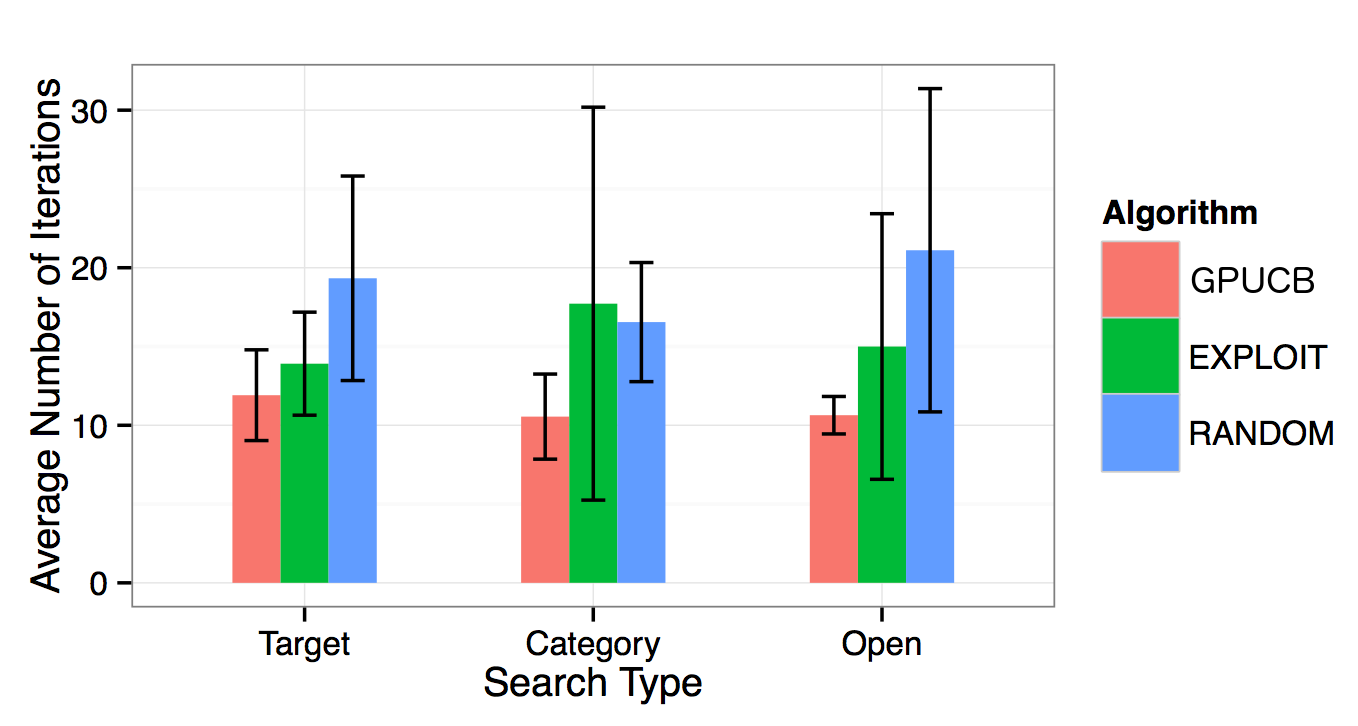
\includegraphics[width=1.0\textwidth]{figures/conf_intr.png}
    \caption{Average number of iterations along with 95\% confidence intervals to complete each type of search with GP-SOM, EXPLOIT and RAND systems.}
    \label{bar_chart}
\end{figure}

Figure \ref{bar_chart} clearly shows that GPUCB outperforms EXPLOIT and RAND in terms of average iterations needed to finish. In all the three major tasks, GPUCB could satisfy users in minimum number of iterations. Moreover, the confidence interval was consistent and small in case of GPUCB, while for EXPLOIT and RAND we see huge confidence interval leading to uncontrolled explorations.

EXPLOIT performed considerably better, almost as good as GPUCB, in target search. This is expected because in target search we specify fixed target, say "a red rose" to the user. If in the first iteration the user gets a red rose and provides maximum feedback possible to it, pure exploitation is the best way to conclude quickly rather than exploring which produces irrelevant images which will never receive feedbacks. Therefore, GPUCB might not be the best option in target search. Category and open ended searches do not have fixed targets, thus require more exploration and GPUCB performed better than EXPLOIT in those cases as seen from Figure \ref{bar_chart}.

\begin{figure}[h!]
  \centering
    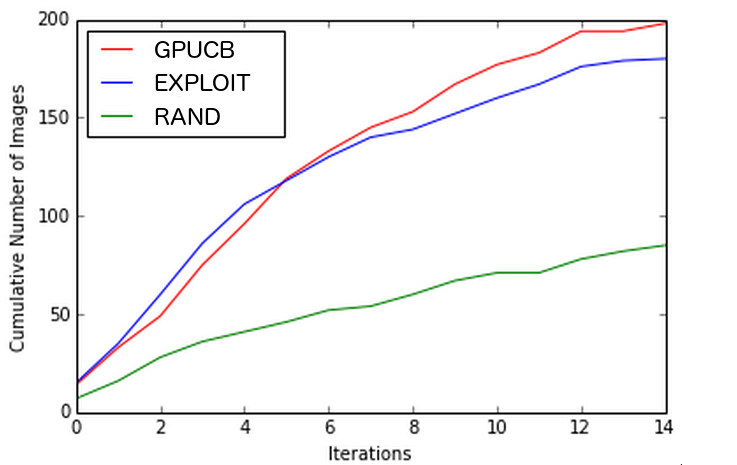
\includegraphics[width=0.32\textwidth]{figures/Target_Positive.png}
    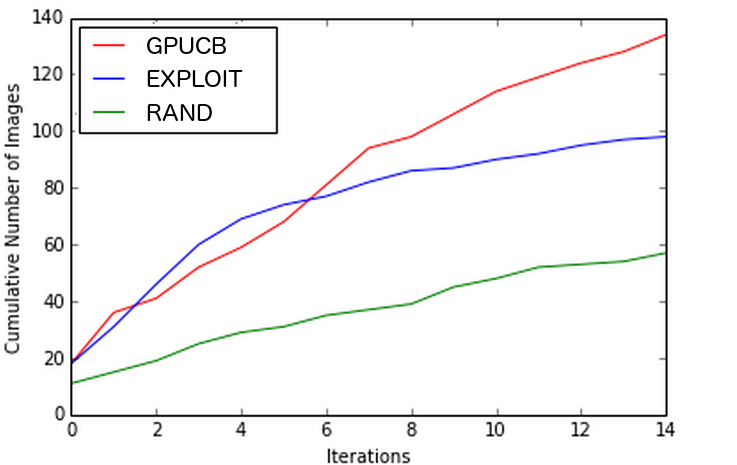
\includegraphics[width=0.32\textwidth]{figures/Category_Positive.png}
    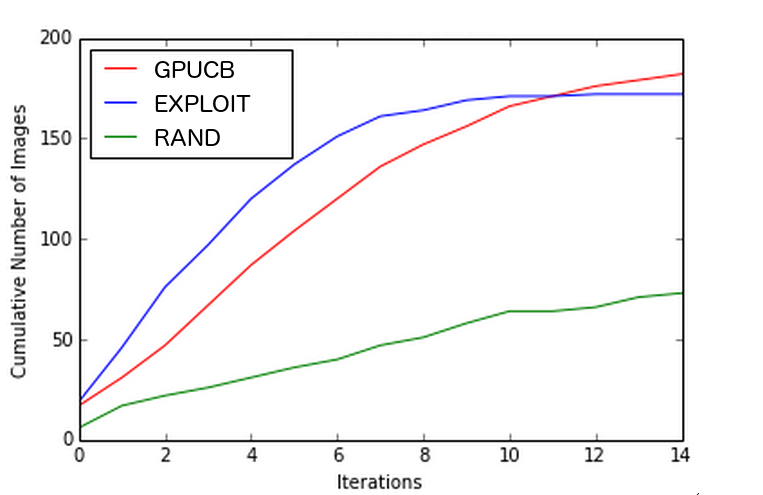
\includegraphics[width=0.32\textwidth]{figures/Open_Positive.png}
    \caption{Cumulative number of images marked as positive by user over iterations for GP-SOM, EXPLOIT and RAND for different type of searches}
    \label{positive_feedback}
\end{figure}

Figure \ref{positive_feedback} shows the cumulative number of images getting positive feedback over the three tasks in all three algorithms. We use unannotated or untagged images, therefore the number of positive feedback over iterations are the only measure of how relevant the images were, presented to the user. As mentioned before, exploration did not affect target search to a great extent, so GPUCB and EXPLOIT generated more or less equal number of positive images. Both in category search and open ended search, GPUCB generated more positive feedback than the other two. In all three tasks, EXPLOIT started producing more positive feedbacks in the initial iterations, as GPUCB produced some irrelevant images due to exploration, but in the end fell behind GPUCB. GPUCB performed well to finish around twenty iterations in target search and fifteen in open ended search. The other two continued. RAND was clearly outperformed by the other two everywhere.

Figure \ref{red_rose_1} and Figure \ref{red_rose_2} show the first two iterations of the experiment for red rose. Clearly the experiment started with images from random colour domains. Figure \ref{red_rose_5} shows how the experiment converged to mostly red dominated colour space with three red roses. Figure \ref{city_night_1} to Figure \ref{city_night_5} show the same for "city by night". It reflects how well GPUCB performed and how more relevant images appeared with later iterations.
\begin{figure}[!h]
  \centering
    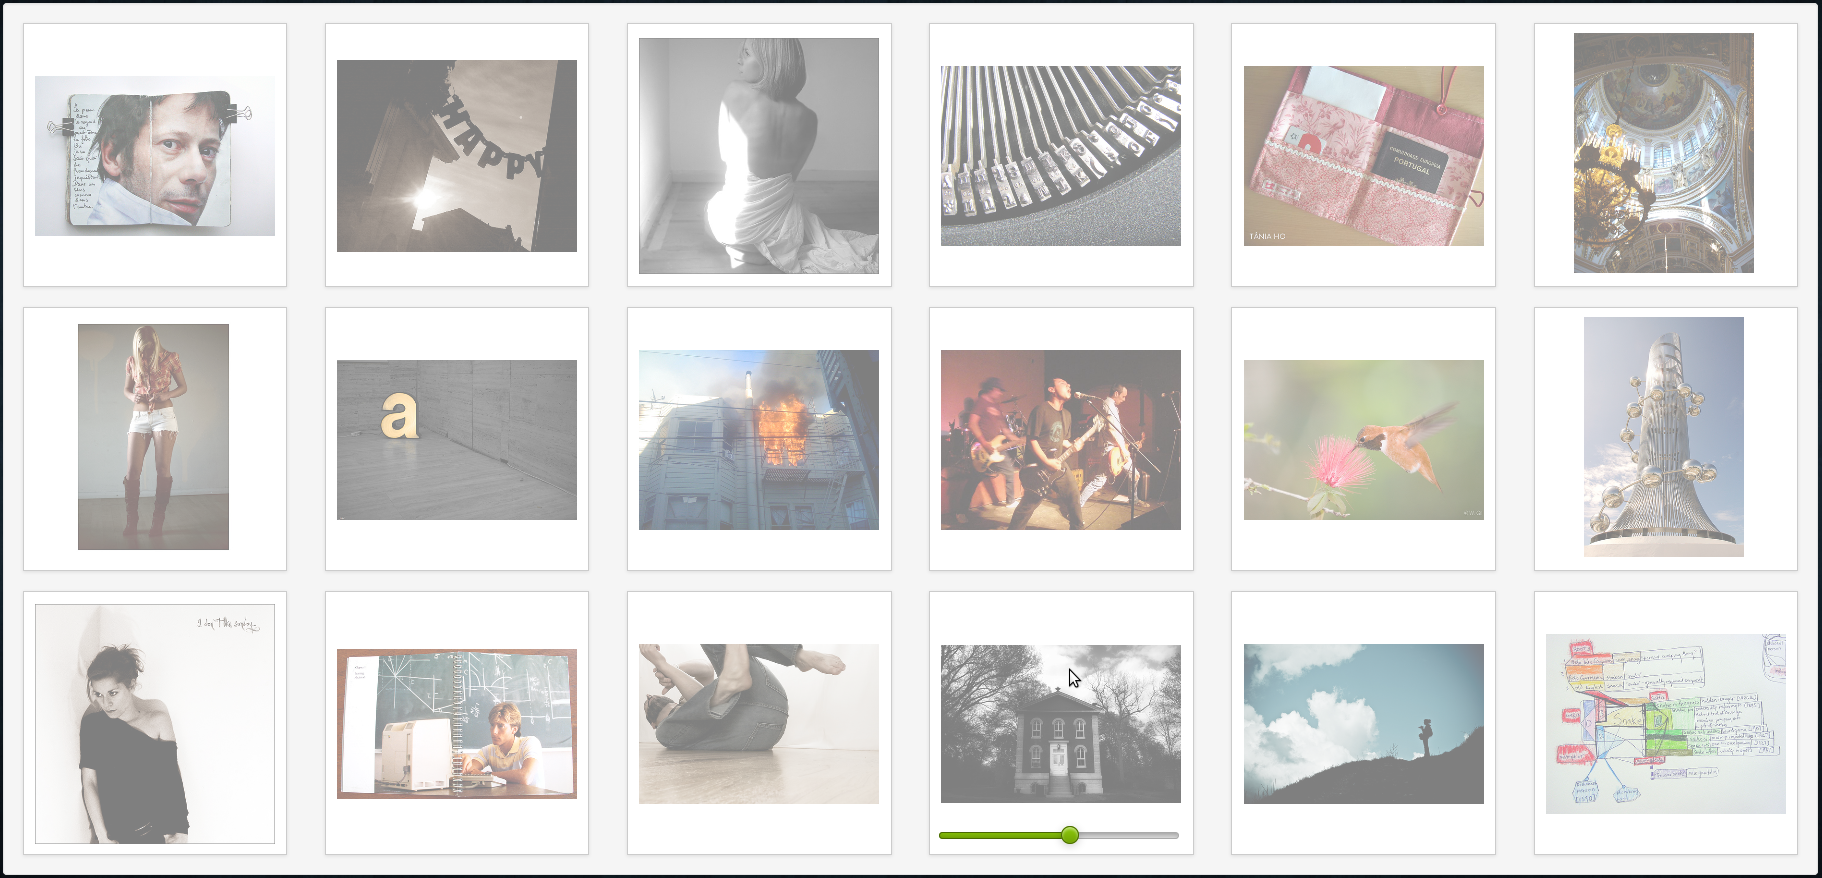
\includegraphics[width=0.90\textwidth,height=6cm]{figures/Rose_1.png}
    \caption{Red Rose Iteration 1}
    \label{red_rose_1}
\end{figure}

\begin{figure}[h!]
  \centering
    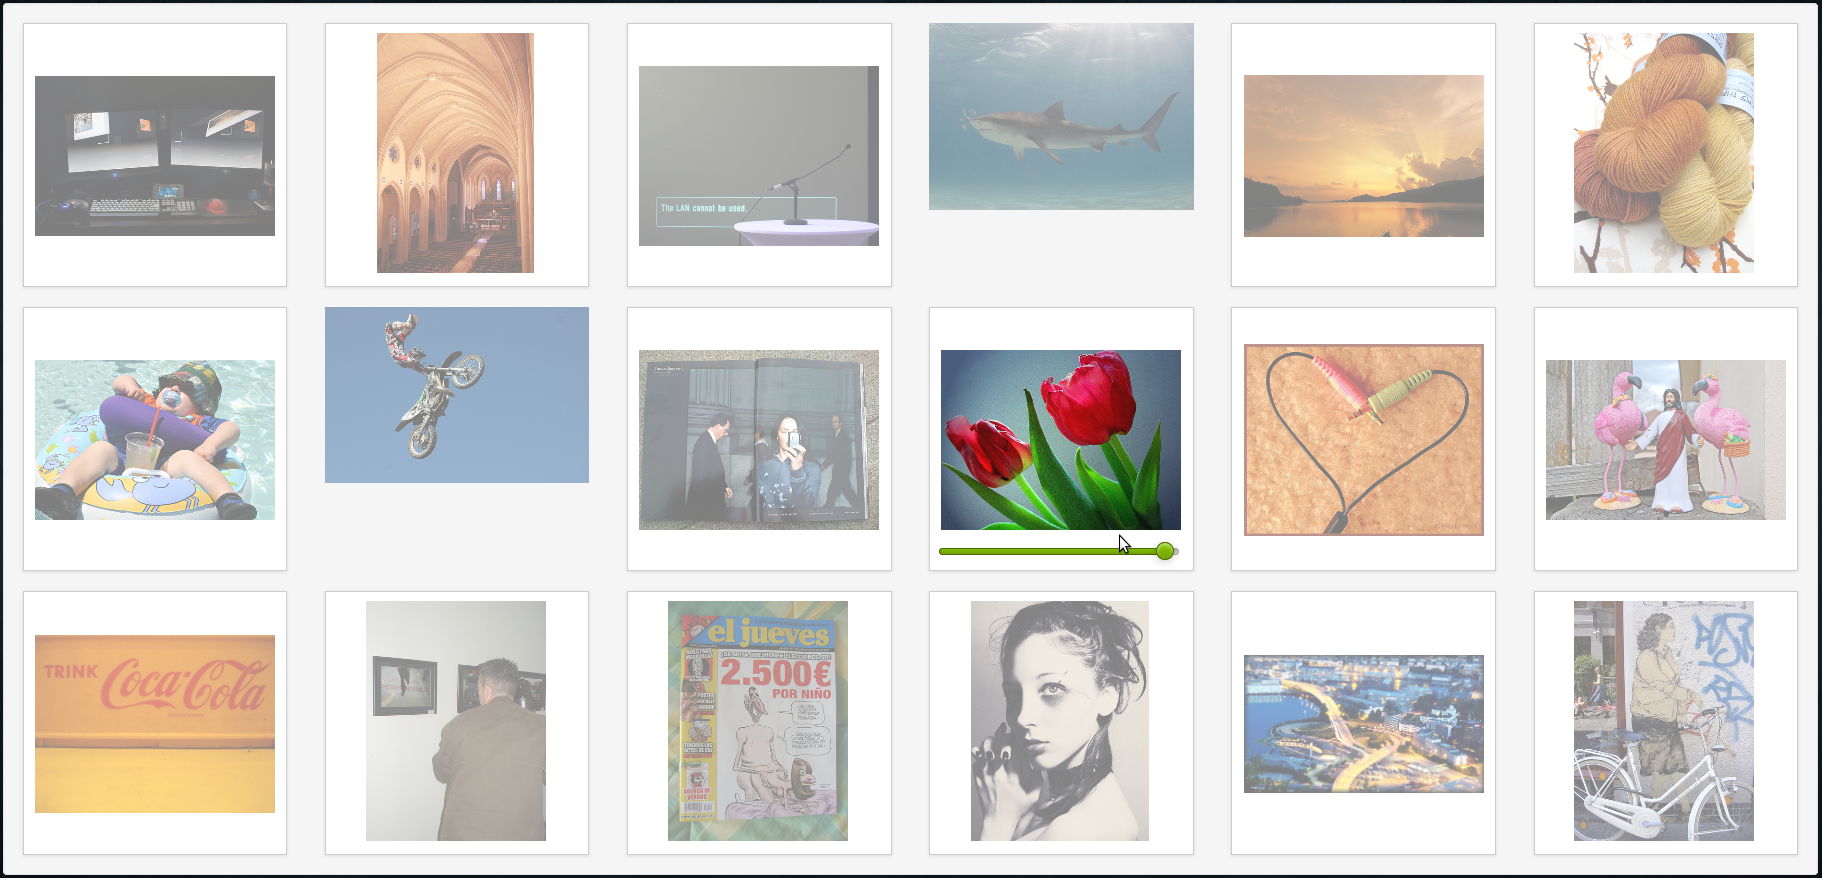
\includegraphics[width=0.90\textwidth,height=6cm]{figures/Rose_2.png}
    \caption{Red Rose Iteration 2}
    \label{red_rose_2}
\end{figure}

\begin{figure}[h!]
  \centering
    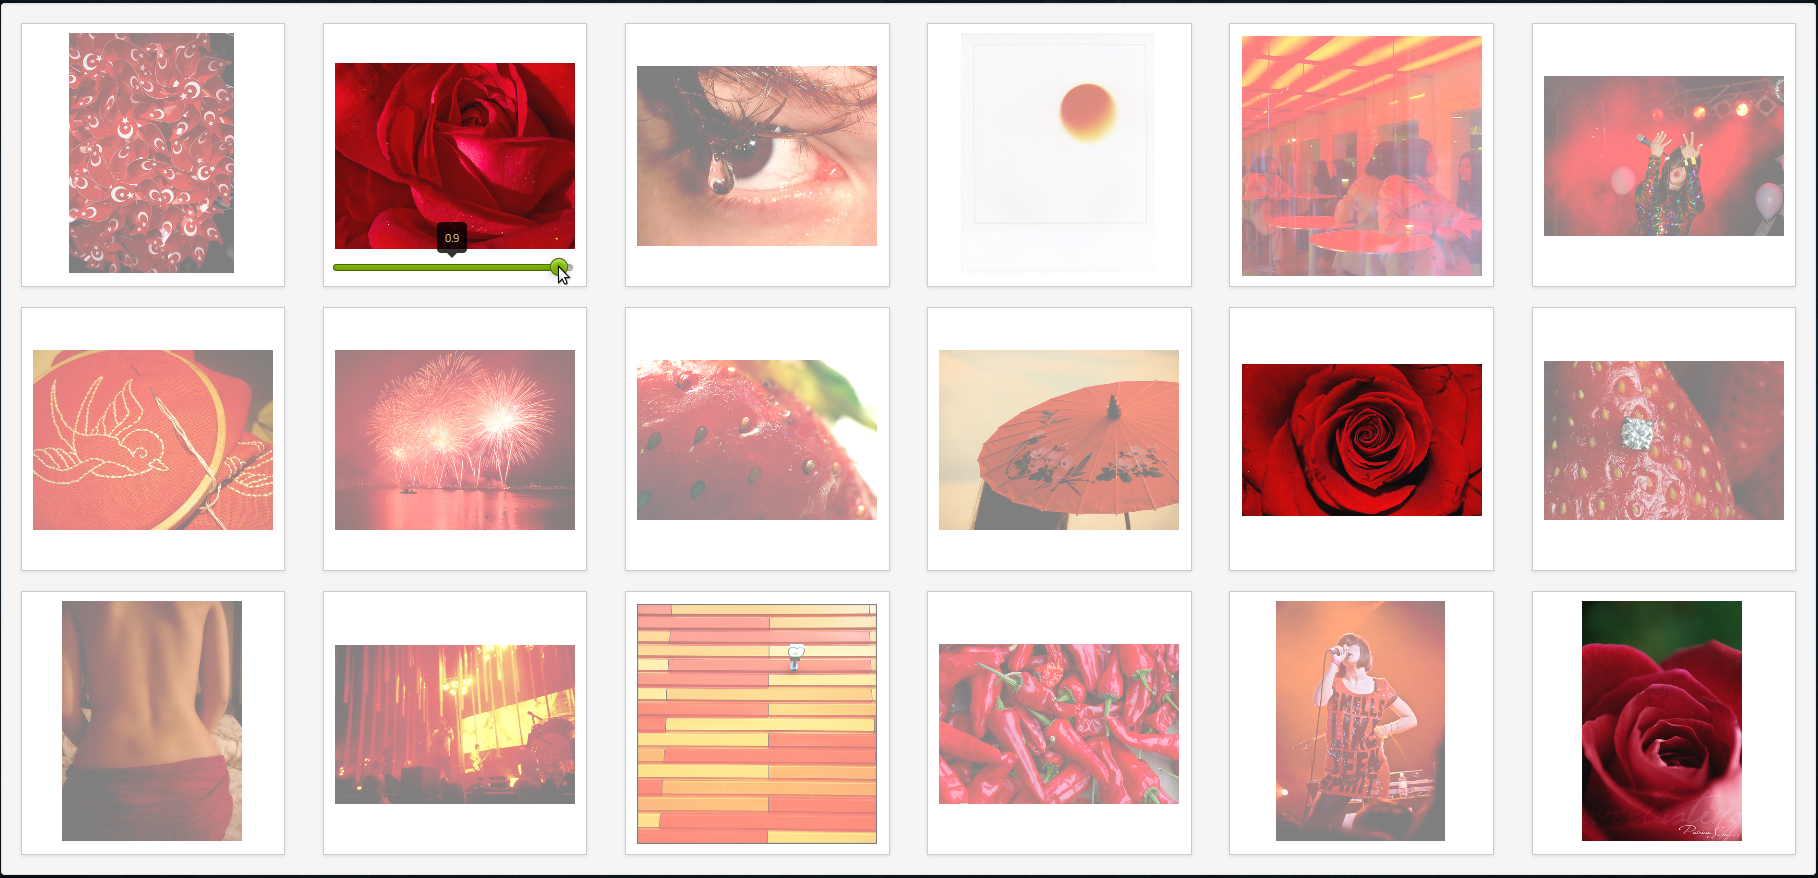
\includegraphics[width=0.90\textwidth,height=6cm]{figures/Rose_5.png}
    \caption{Red Rose Iteration 5}
    \label{red_rose_5}
\end{figure}


\begin{figure}[!h]
  \centering
    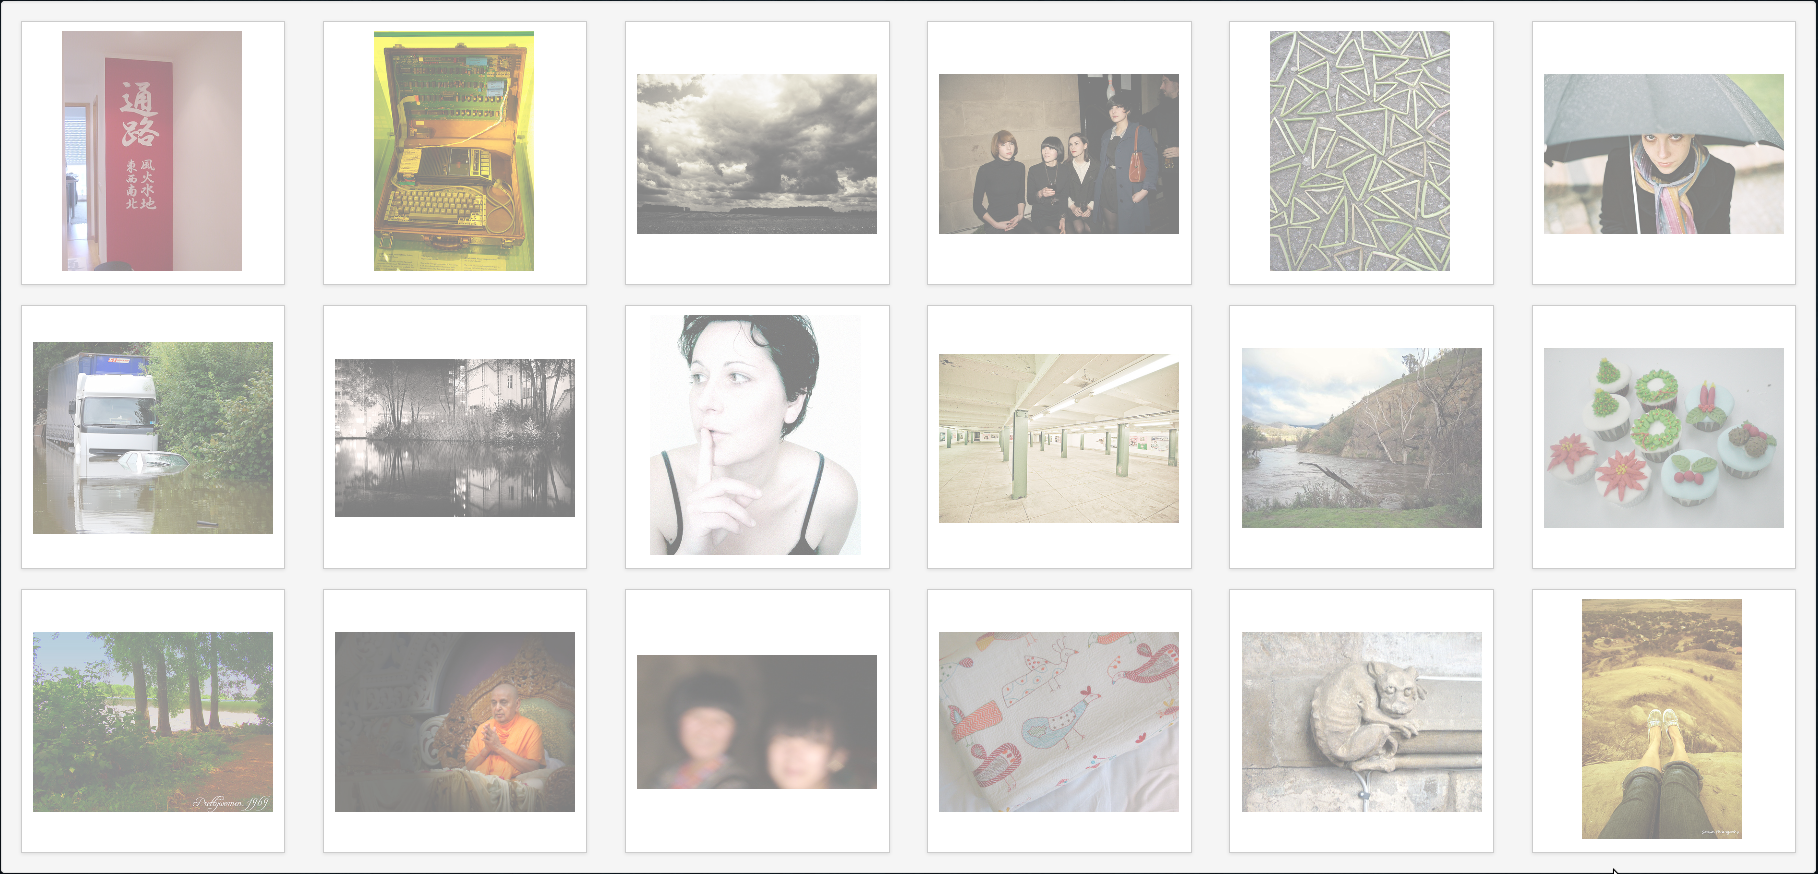
\includegraphics[width=0.90\textwidth,height=6cm]{figures/City_Night_1.png}
    \caption{City by Night Iteration 1}
    \label{city_night_1}
\end{figure}

\begin{figure}[h!]
  \centering
    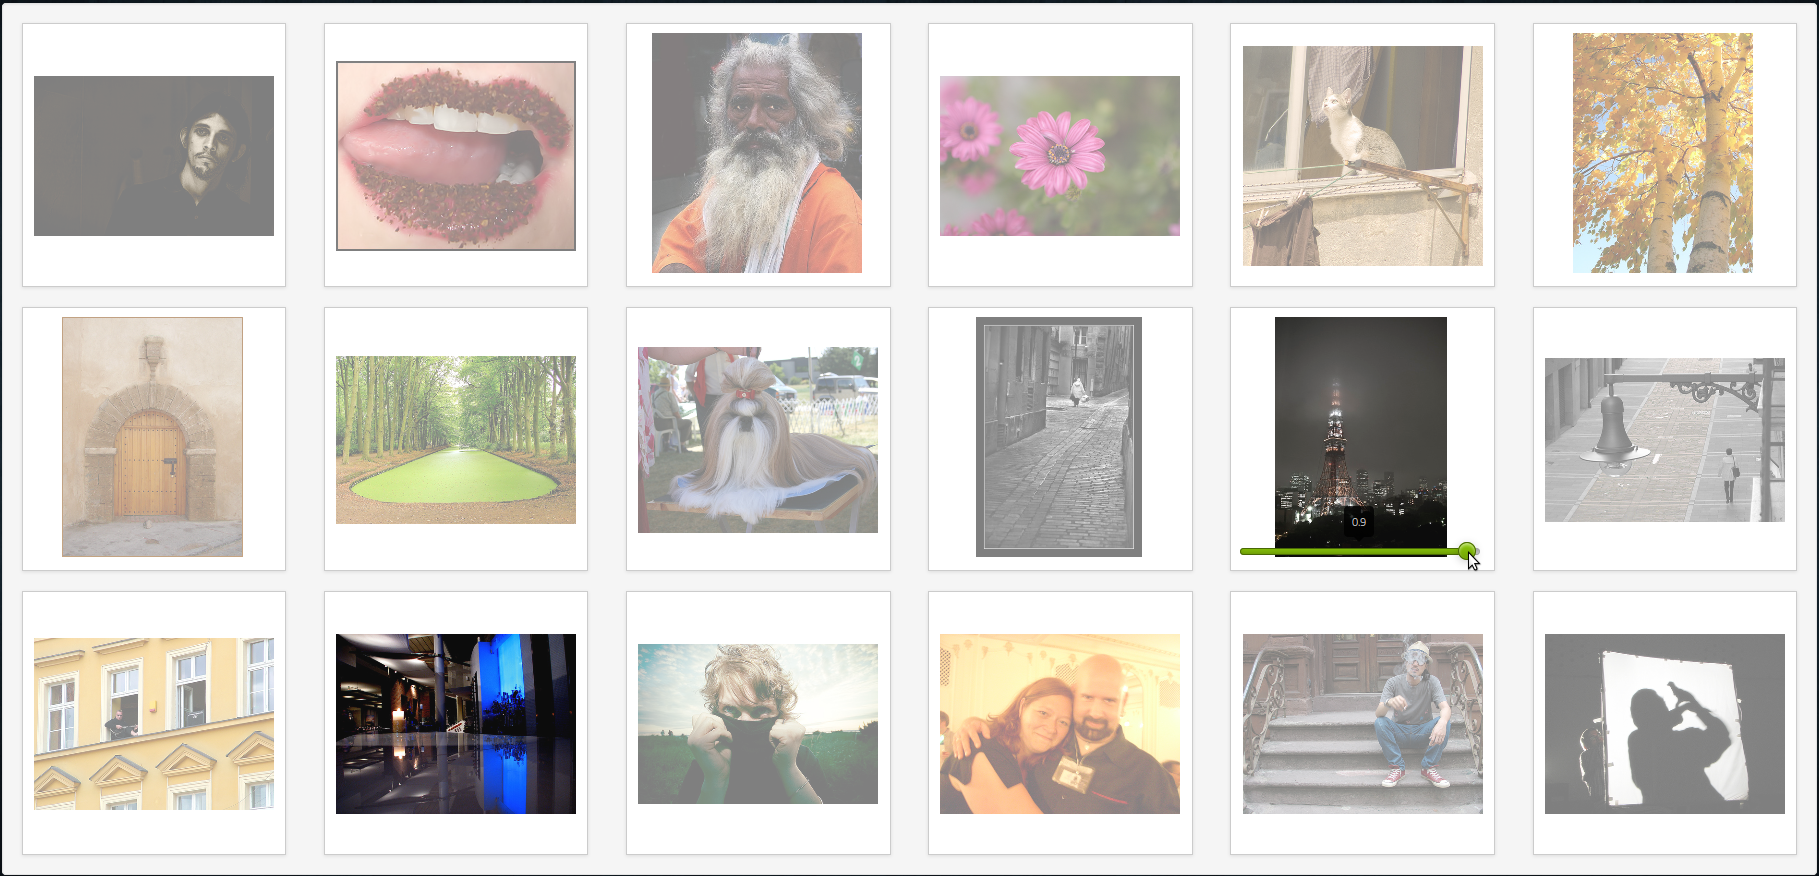
\includegraphics[width=0.90\textwidth,height=6cm]{figures/City_Night_2.png}
    \caption{City by Night Iteration 2}
    \label{city_night_2}
\end{figure}

\begin{figure}[h!]
  \centering
    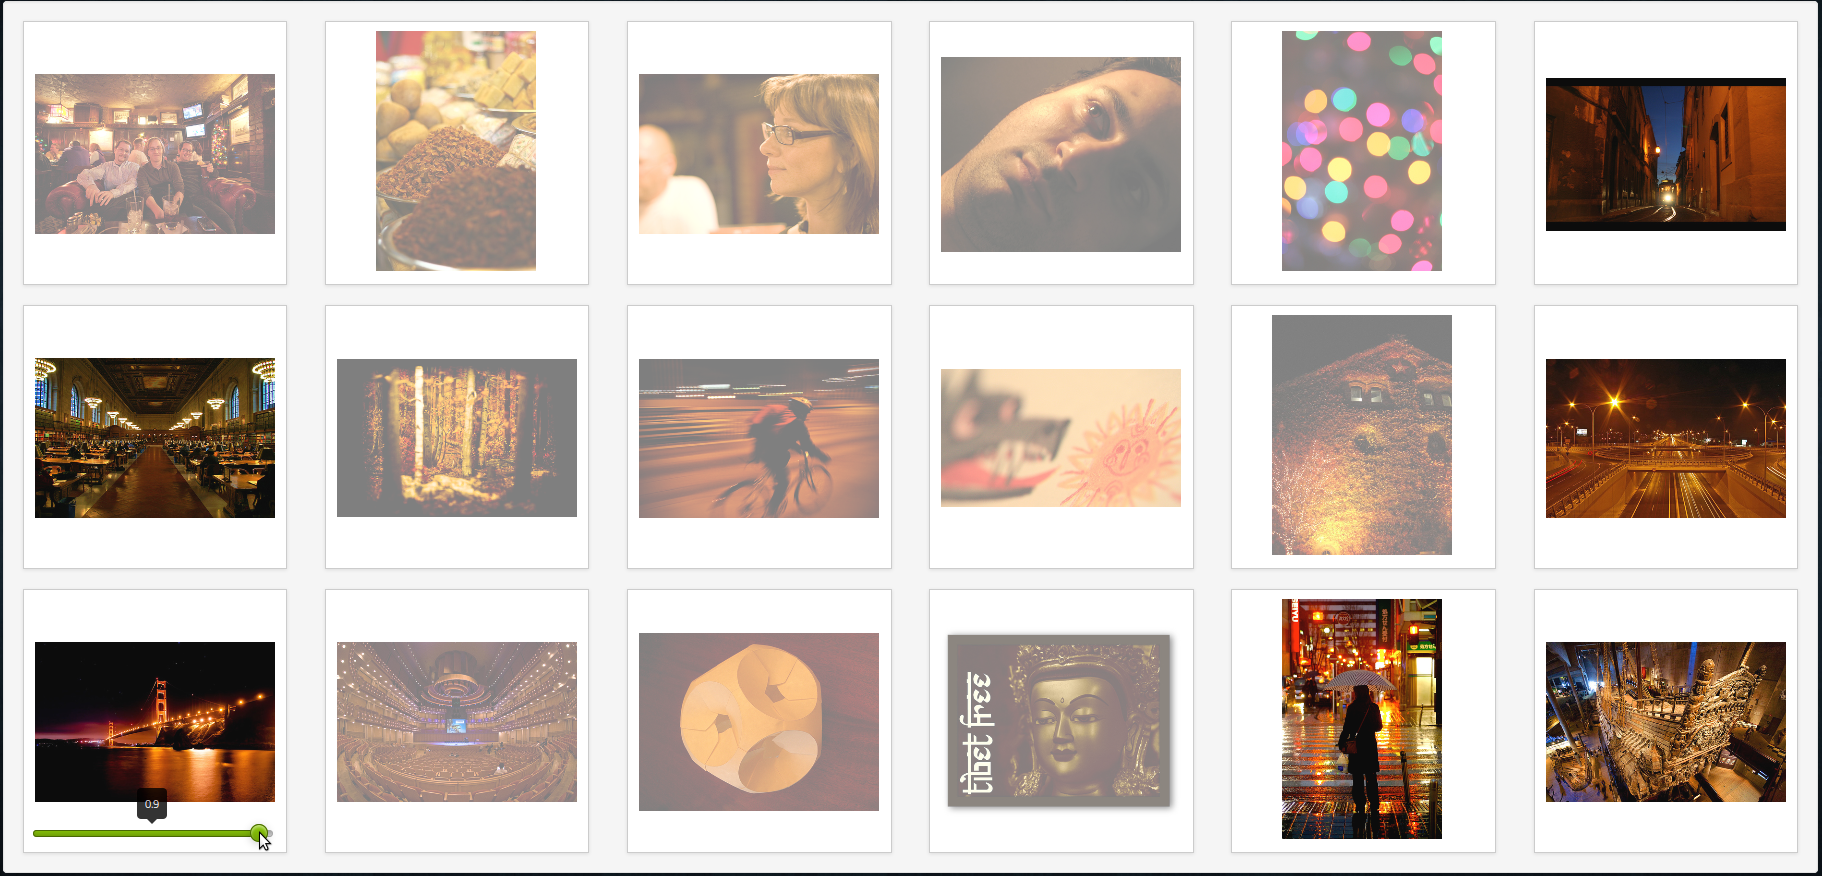
\includegraphics[width=0.90\textwidth,height=6cm]{figures/City_Night_5.png}
    \caption{City by Night Iteration 5}
    \label{city_night_5}
\end{figure}


\section{Discussion}

We have noticed issues from the results. Next, we present them one by one.

\begin{enumerate}
	\item One of the major issues is the applicability of GPUCB. It could not outperform EXPLOIT in target search. The reason is, once the user provides feedback to a suitable image, say a "red rose", EXPLOIT will bring more red roses only. The probability that the user will like one of them the most and finish the search is highest in case of EXPLOIT. The exploration in GPUCB here might introduce some irrelevant images, thus prolonging the process of getting the most suitable "red rose". On the contrary, sometimes it might be extremely useful to have exploration in target search. As we are showing random images initially, it might so happen that the user got no red, but a few reddish yellow images while starting. Assuming a reddish yellow to be the closest available match, the user gave feedback to that. It is highly probable that EXPLOIT would bring up only reddish yellow images afterwards. Only exploration could bring up red images again to direct the search towards a positive end.
	\item As the first iterations for both red rose (Figure \ref{red_rose_1}) and city by night (Figure \ref{city_night_1}) show images randomly, it might so happen that completely irrelevant images had been shown requiring the experiment to restart \label{issue_random_initial_images}.
	\item The system was slow in fetching images because gaussian process took a long time to run on CPU \label{issue_CPU_slow}.
	\item Once the user gives all the feedback he wants and moves to the next iteration, it might so happen that the outcome is not very favourable and the user might want to change some of the previous feedback. But it is not possible to go back and change the feedbacks \label{issue_single_view}.
\end{enumerate}


\section{Corrective measures}

We have taken corrective measures to fix problems \ref{issue_random_initial_images}, \ref{issue_CPU_slow} and \ref{issue_single_view} mentioned above. They are described below.

\begin{figure}[h!]
  \centering
    \includegraphics[width=1.0\textwidth]{figures/Imse_System_Diagram_2}
    \caption{System diagram with GP on GPU}
    \label{system_diagram_2}
\end{figure}

\begin{enumerate}
	\item Problem \ref{issue_random_initial_images} is fixed by setting the initial set of images fixed for a particular task. Say for red rose, whenever it runs irrespective of users, the first set of shown images is the same always. This measure is taken for this set of experiments only. Otherwise in the ready system, for any given task, any user should start from a random set, as predefining a static set of image for each and every possible task the user can go for is not possible.
	\item Problem \ref{issue_CPU_slow} is solved by the introduction of GPU. We no longer use the two-phase Gaussian process model. Neither we have the image clusters anymore. Rather we run Gaussian process once on the entire set of images as shown in Figure \ref{system_diagram_2}. After calculating the UCB values over the test set of images, instead of picking up one image at a time, we choose the first 12 images from the sorted UCB values. This way we save time from running the Gaussian process several times per iteration. Running Gaussian process over the entire image set (images not shown so far) takes an unaffordable amount of time on CPU but using GPU eliminates the problem. Also we do not pre-calculate the entire kernel, rather we push the input vectors (shown and not-shown image indices) into the GPU which calculates those required parts of the kernel matrix runtime. The GPU is fast enough to do that.
	\item Problem \ref{issue_single_view} is solved by the introduction of a new interface called FutureView described below.
 
\end{enumerate}




\subsection{FutureView}

In this experiment we introduce a new interface which helps eliminating the problem of users not being able to go back and change feedback if required. We split the screen into two sections, the left one having a width of 70\% and the right one 30\%. The left section has exactly the same structure of the display panel from the previous experiment but the right section is what we refer to as the FutureView. It also displays images but images here do not have any sliding-feedback controls and images appear a bit faded out. This view shows what images are going to appear in the next iteration if the user keeps the current feedback which is given to the images in the left section.

\begin{figure}[h!]
  \centering
    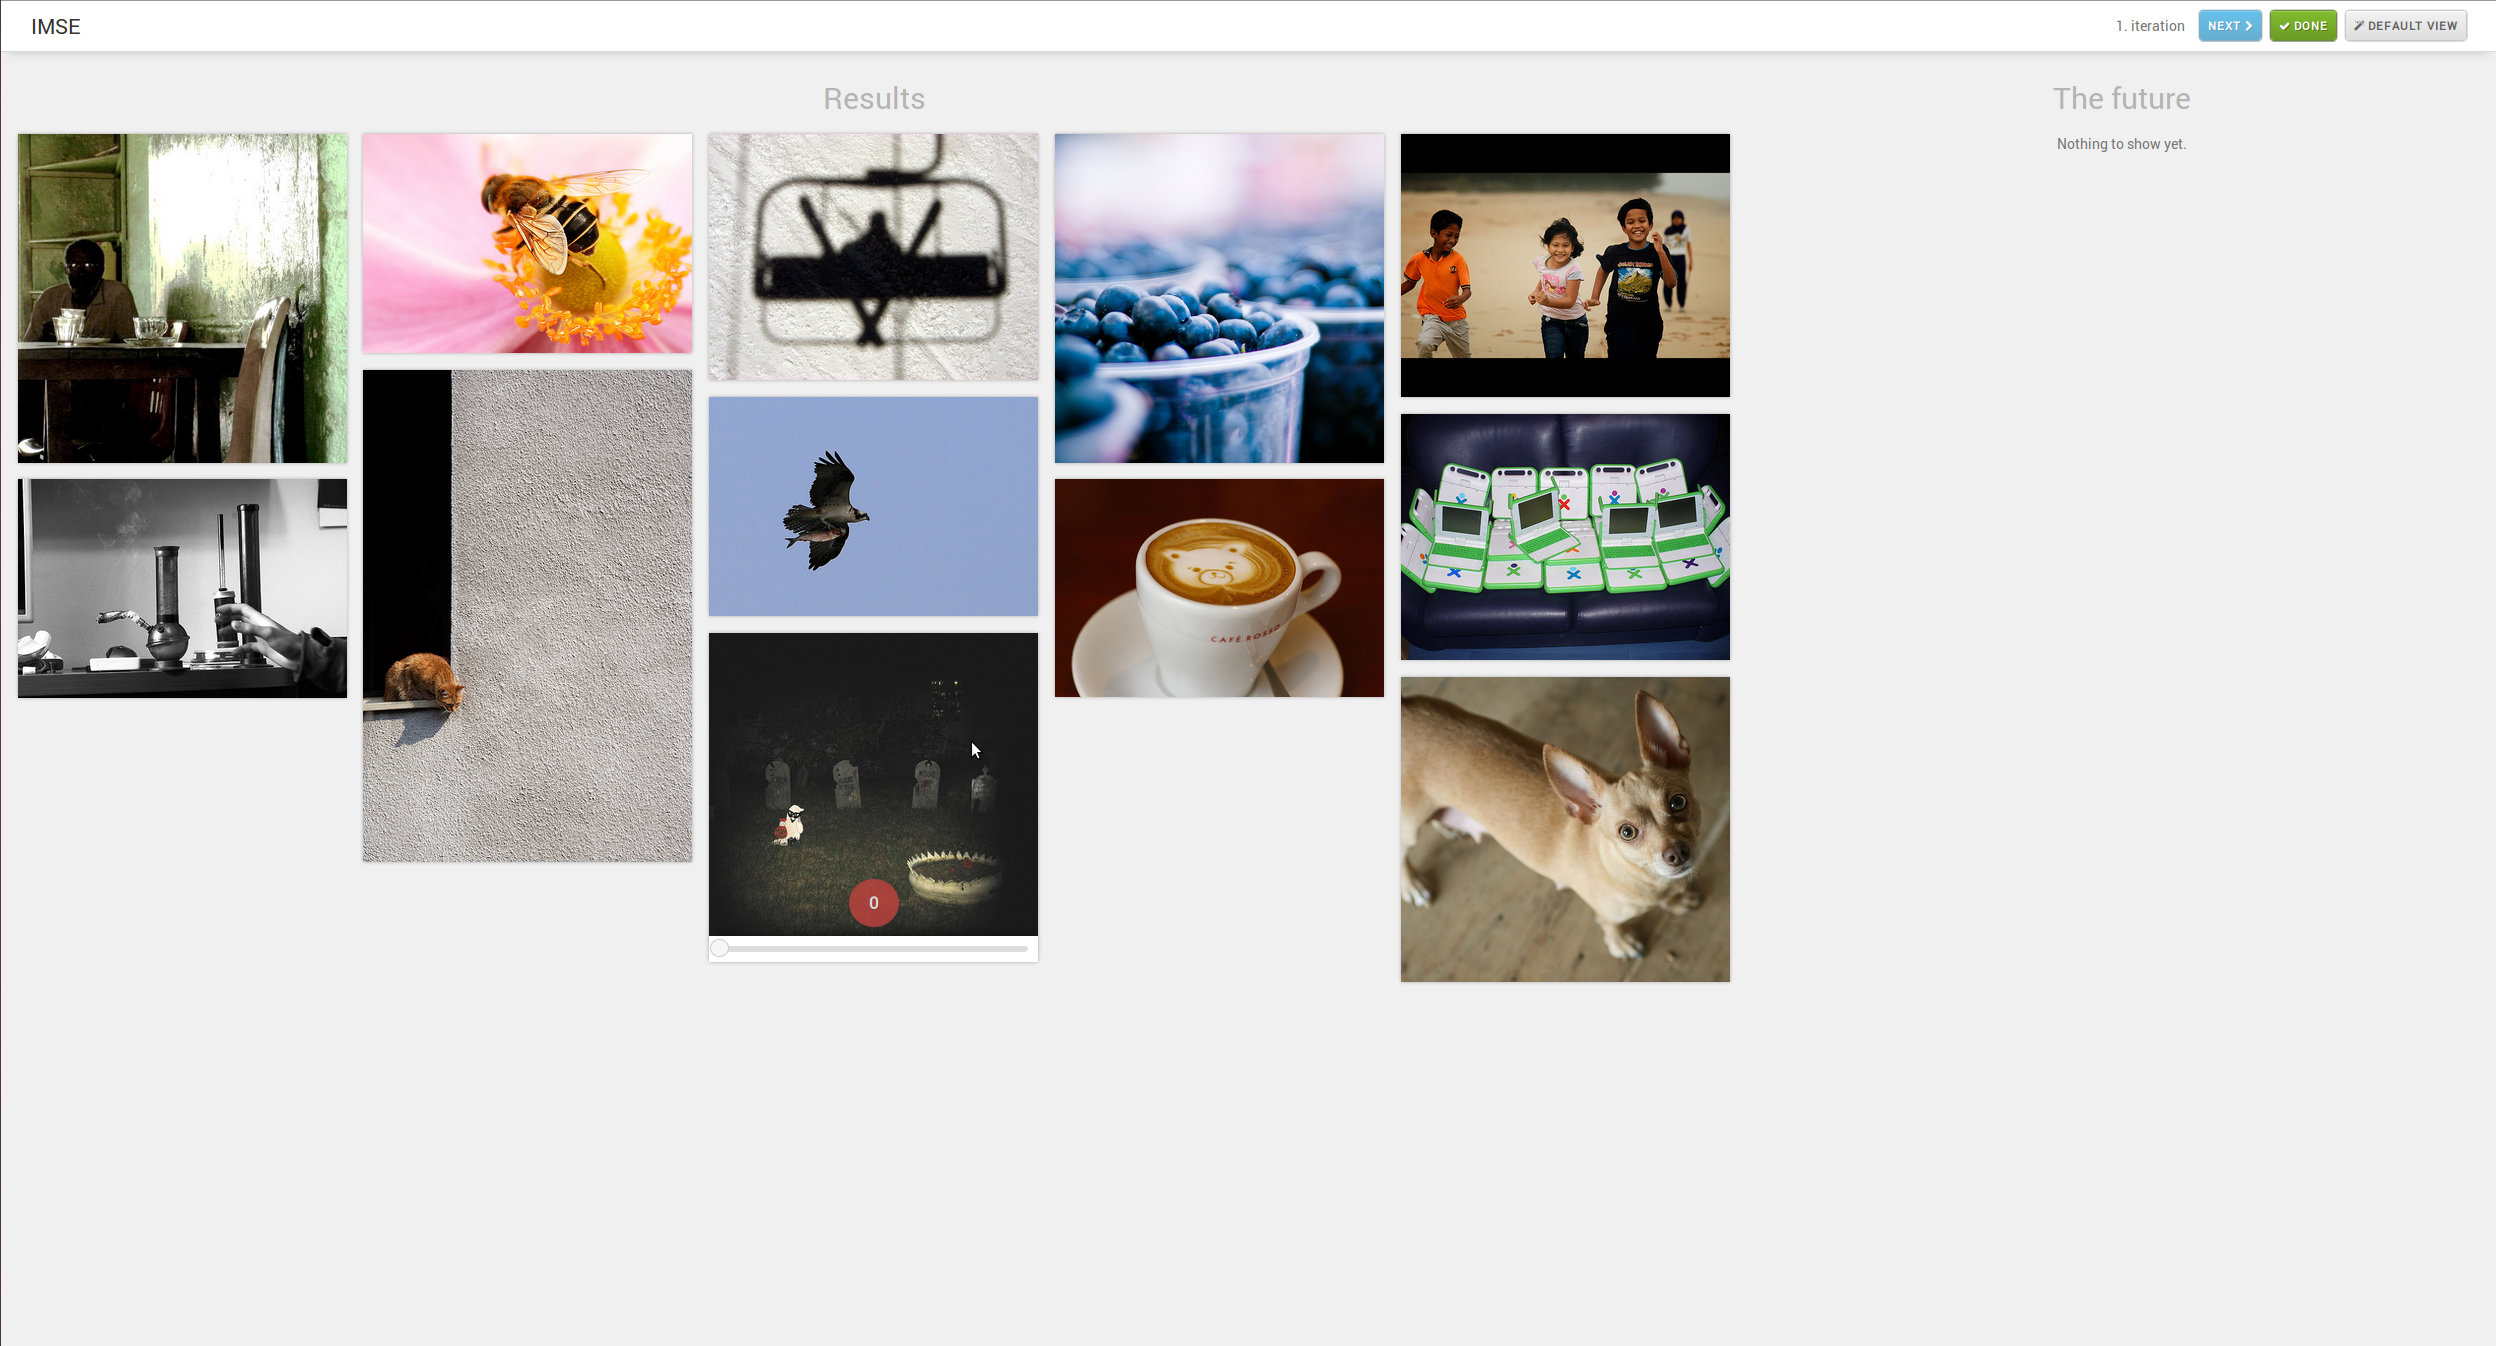
\includegraphics[width=0.90\textwidth,height=6cm]{figures/future_sample_1.jpg}
    \caption{Empty FutureView}
    \label{fut_samp_1}
\end{figure}

\begin{figure}[h!]
  \centering
    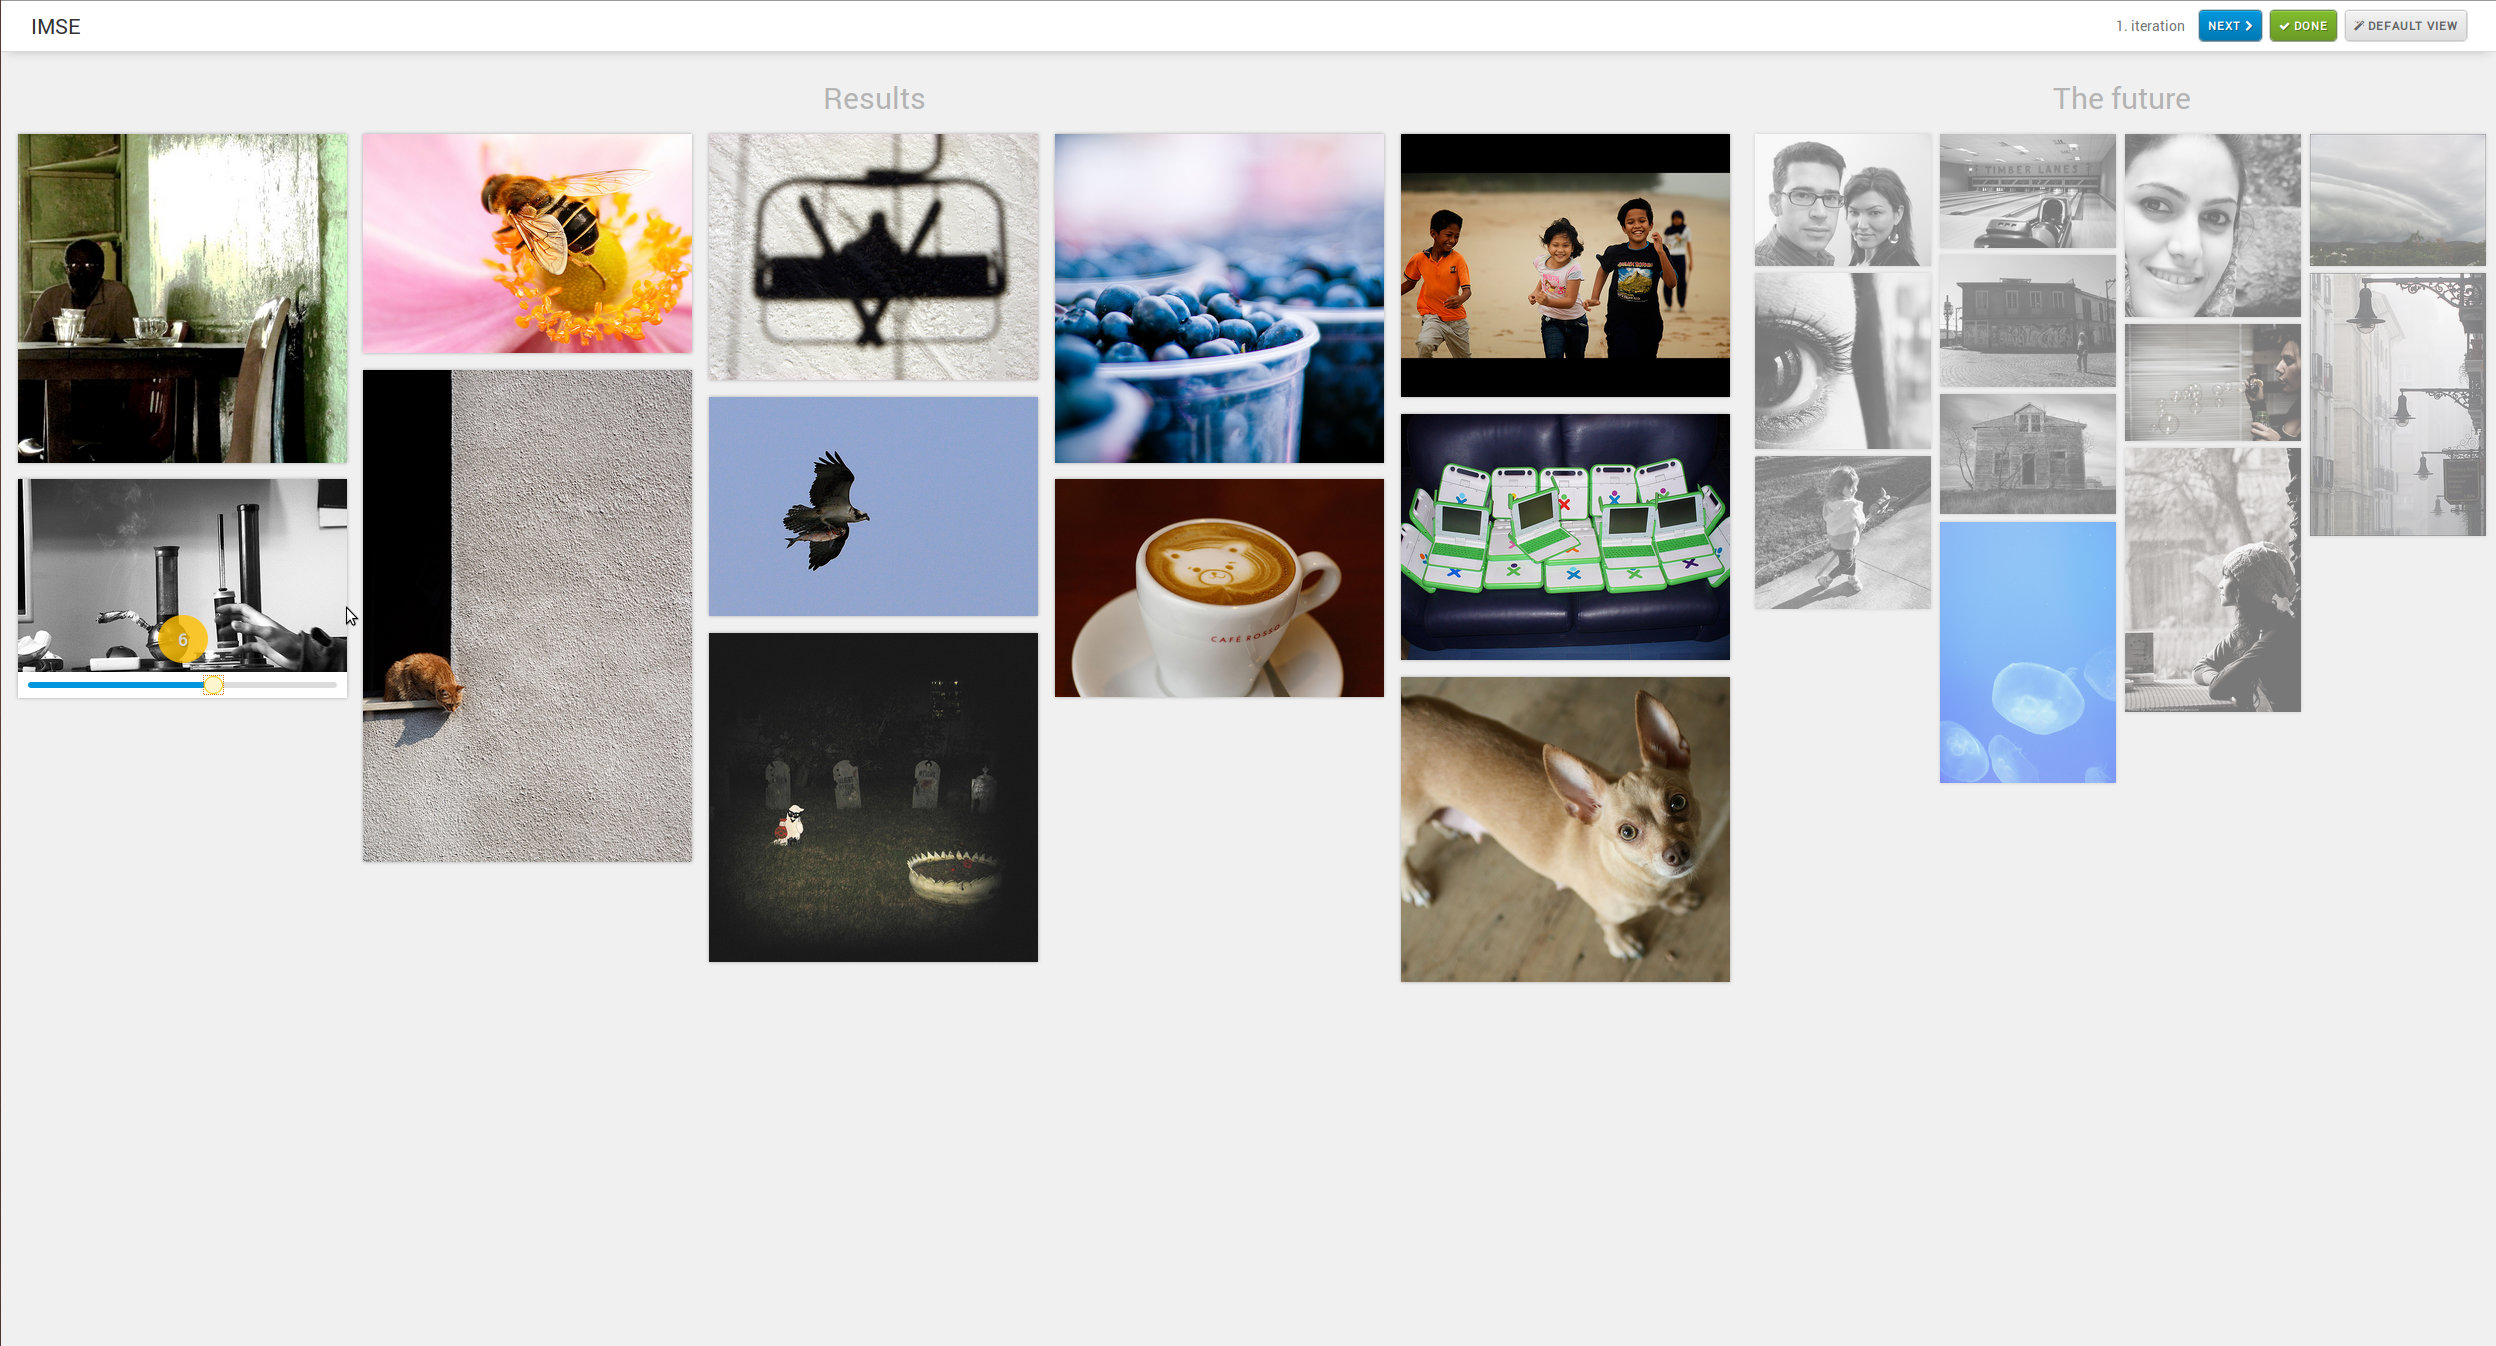
\includegraphics[width=0.90\textwidth,height=6cm]{figures/future_sample_2.jpg}
    \caption{FutureView with images to be displayed in the next iteration}
    \label{fut_samp_2}
\end{figure}

Therefore, the user sees an early view of the next iteration. If images there are not suitable, the user can change the feedback and get new images. Once the user feels that the images in the FutureView are suitable, he can go next and the images from the FutureView will replace the images in the left section. We will refer to this as current view from now on, and the same procedure follows. Initially each iteration starts with an empty FutureView as shown in Figure \ref{fut_samp_1} and as soon as the user gives one feedback, the FutureView fills up with images based on that feedback. Whenever the user gives feedback to any of the images in the current view, the FutureView gets refreshed with new images as shown in Figure \ref{fut_samp_2}.

\subsection{Experimental setup}

We aim to measure the effectiveness of FutureView in terms of 1) The amount of time taken to finish an experiment, 2) The number of positive feedback generated throughout the experiment, 3) The mental and physical stress of the user in performing the task and 4) Whether the user finishes a task successfully by finding the appropriate image. For a particular task we show a predefined static set of images whenever the task is performed.

\subsection{Participants}

We recruited 12 participants from the university with average age 24 (maximum 30, minimum 20). Three of these participants were females. Most of these participants were students, researchers and professionals in the field of computer science, one of them a mathematician.





\subsection{Tasks}

The tasks were divided into three broad genres, target search, category search and open ended search, as before. We had two tasks in each of these genre,

\begin{itemize}
	\item Target Search: Red Rose, Tall Building
	\item Category Search: City by Night, Seashore
	\item Open Ended Search: Happiness, Gardening
\end{itemize}

Our goal was to run a comparative study between the traditional view (current view) and FutureView over the same backend system to see which one performs better in terms of user satisfaction, task duration for an entire search session, amount of exploration over the image space etc.

We designed the experiments so that each participant had to perform 6 distinct tasks (Red Rose, Tall Building, City by Night, Seashore, Happiness and Gardening) altogether three being on the FutureView and the rest otherwise. We ensured each participant performed only one task from each genre on each system (we refer to the current view and FutureView as two distinct systems), thus any participant who performed the task of red rose on current view, had to perform the task of tall building on FutureView as these two are from the same genre (target search). These scheme was followed for all three genres. This way we ensured that each participant performed three task (one from each genre) on single view and the rest, the other three task on FutureView. This way we had $12 \times 3 = 36$ tasks performed on single view and $36$ tasks performed on FutureView. This also ensured that each task was performed $6$ times on each system.

\begin{table}[h]
    \begin{tabular}{ |l|l|l| }
		\hline
		User serial number & Task performed on Single View & Task performed on FutureView \\ 
		\hline
		\multirow{3}{*}{1} & Red Rose & Tall Building \\
 			& City by Night & Seashore \\
 			& Happiness & Gardening \\
 		\hline
 		\multirow{3}{*}{2} & Red Rose & Tall Building \\
 			& Seashore & City by Night \\
 			& Gardening & Happiness \\
 		\hline
		\multirow{3}{*}{3} & Red Rose & Tall Building \\
 			& City by Night & Seashore \\
 			& Happiness & Gardening \\
 		\hline
 		\multirow{3}{*}{4} & Red Rose & Tall Building \\
 			& Seashore & City by Night \\
 			& Gardening & Happiness \\
 		\hline
 		\multirow{3}{*}{5} & Red Rose & Tall Building \\
 			& City by Night & Seashore \\
 			& Happiness & Gardening \\
 		\hline
 		\multirow{3}{*}{6} & Red Rose & Tall Building \\
 			& Seashore & City by Night \\
 			& Gardening & Happiness \\
 		\hline
 		\multirow{3}{*}{7} & Red Rose & Tall Building \\
 			& Seashore & City by Night \\
 			& Gardening & Happiness \\
 		\hline
 		\multirow{3}{*}{8} & Red Rose & Tall Building \\
 			& City by Night & Seashore \\
 			& Happiness & Gardening \\
 		\hline
 		\multirow{3}{*}{9} & Red Rose & Tall Building \\
 			& Seashore & City by Night \\
 			& Gardening & Happiness \\
 		\hline
 		\multirow{3}{*}{10} & Red Rose & Tall Building \\
 			& City by Night & Seashore \\
 			& Happiness & Gardening \\
 		\hline
 		\multirow{3}{*}{11} & Red Rose & Tall Building \\
 			& Seashore & City by Night \\
 			& Gardening & Happiness \\
 		\hline
 		\multirow{3}{*}{12} & Red Rose & Tall Building \\
 			& City by Night & Seashore \\
 			& Happiness & Gardening \\
 		\hline
	\end{tabular}
	\caption{Task distribution per user}
    \label{table:table_task_allocation}
\end{table}


In the previous experiment, described in \ref{experiment_1}, we had a random initial set to start with. But that led to having different impacts on the same task performed by different users. In this experiment, for each task, we kept a static initial set of images which could lead a user to the destination easily within $30$ iterations. The task allocation is shown in Table \ref{table:table_task_allocation}. For each user and system combination, the three tasks were presented to the user one after another in a random permutation.

We used a Tobii X2-60 eye tracker with sampling rate of 60Hz, to measure how much time a user spends to look at the FutureView, to analyse how a particular search is affected by the user's approach to the FutureView. Here, we measure the amount of time the user spent looking at the FutureView. This measure gives us the idea, whether the user actually used the FutureView or not.


\subsection{Procedure}


Each participant was given an instruction sheet to go through before the study. We wanted to keep a record of how each individual user is familiar with searching for images on a computer, what they look for in general and which image search engines they use etc. for later reference and better understanding of their background in using such systems. Thus, we set up a Warm Up questionnaire in google form as follows,

\begin{itemize}
	\item How often do you search for images?
	\item How often do you search for images for work?
	\item How often do you search for images for leisure?
	\item What kind of images do you often search for?
	\item What are the image search systems you have used so far? Regular search engines or something more specific?
	\item What difficulties did you find in using traditional image search systems you have used?
	\item What changes you would be happy to see in your favourite image search engines?
\end{itemize}


Each user was asked to complete the above mentioned questionnaire in the beginning. After a user filled up the questionnaire and read the instructions, they were given a consent form to sign. The user was then introduced to both the systems and led through two training tasks on each of the systems. Once the user felt familiar, we calibrated the eye tracker and started logging user's gaze. Next, we started the actual experiments. Six tasks were presented to the user in a random order. After finishing each task, the user had to fill up a task usability questionnaire (modelled after NASA TLX questionnaire \cite{NASA_TLX}) and after every three tasks, i.e. after three experiments finished with each system, the user had to fill up a system usability questionnaire (modelled after SUS questionnaire \cite{sus}). After all the six tasks were finished, the eye tracker log was saved and we conducted a small interview with the user with mostly the following questions asked,

\begin{itemize}
	\item How was your experience with this system?
	\item How interesting was the system to use?
	\item Did you notice anything different, exciting, worth mentioning in this system that you did not see in other commercial image search systems you have used?
	\item Was the FutureView useful?
	\item Was the FutureView easy to use?
	\item Did the FutureView help you to reach your destination more quickly than the single view?
	\item What prospect do you see in this system if we make it a commercial one?
	\item Will you personally use this system regularly if we make it live on the internet?
	\item Do you feel any major functionality that an image search system should have and present in commercial systems, missing in our system?
	\item What suggestions for modifications, improvements do you have for this system?
\end{itemize}

\section{Results}

For each experiment we saved the following,

\begin{itemize}
	\item number of iterations to complete each task
	\item start time of experiment
	\item running time
	\item images shown
	\item feedbacks received
	\item feedback timestamps
	\item end time of experiment
\end{itemize}

From this information we calculated the average iterations per experiments, average running time per iteration of experiments, average total running time of an entire experiment and average number of feedback received per experiment. Table \ref{table:exp_mean_std_genre} shows genre wise mean and standard deviation of all the parameters we calculated. Sometimes due to outliers or sample sizes, mean and variance of two datasets differs but they follow the same data distribution. We need to show that two datasets have significant statistical differences to say that they are actually different. Here, we used \textit{Wilcoxon signed-rank test} \cite{nonparam_stats} to determine whether the data generated by both FutureView and single view for each experiment and measurement have enough statistical differences or not. Table \ref{table:exp_wilcoxon_genre} shows the wilcoxon P value for each of the parameters comparing the FutureView and the single view. From Table \ref{table:exp_mean_std_genre} we see that the mean total running time is nearly equal in both the FutureView and single view but the average total images shown is much higher in FutureView than in single view across all the genres. We see from Table \ref{table:exp_wilcoxon_genre} that the P value is less than 0.05 in case of open and target searches, marginally over 0.05 in category search for total shown images and significantly greater than 0.05 for total duration. It supports the claim that total shown images is considerably higher in case of FutureView though it takes almost equal amount of time to finish. Therefore, the FutureView allows much higher exploration in a lesser amount of time. Figure \ref{dur_vs_img} reflects the same.

\begin{figure}[h!]
  \centering
    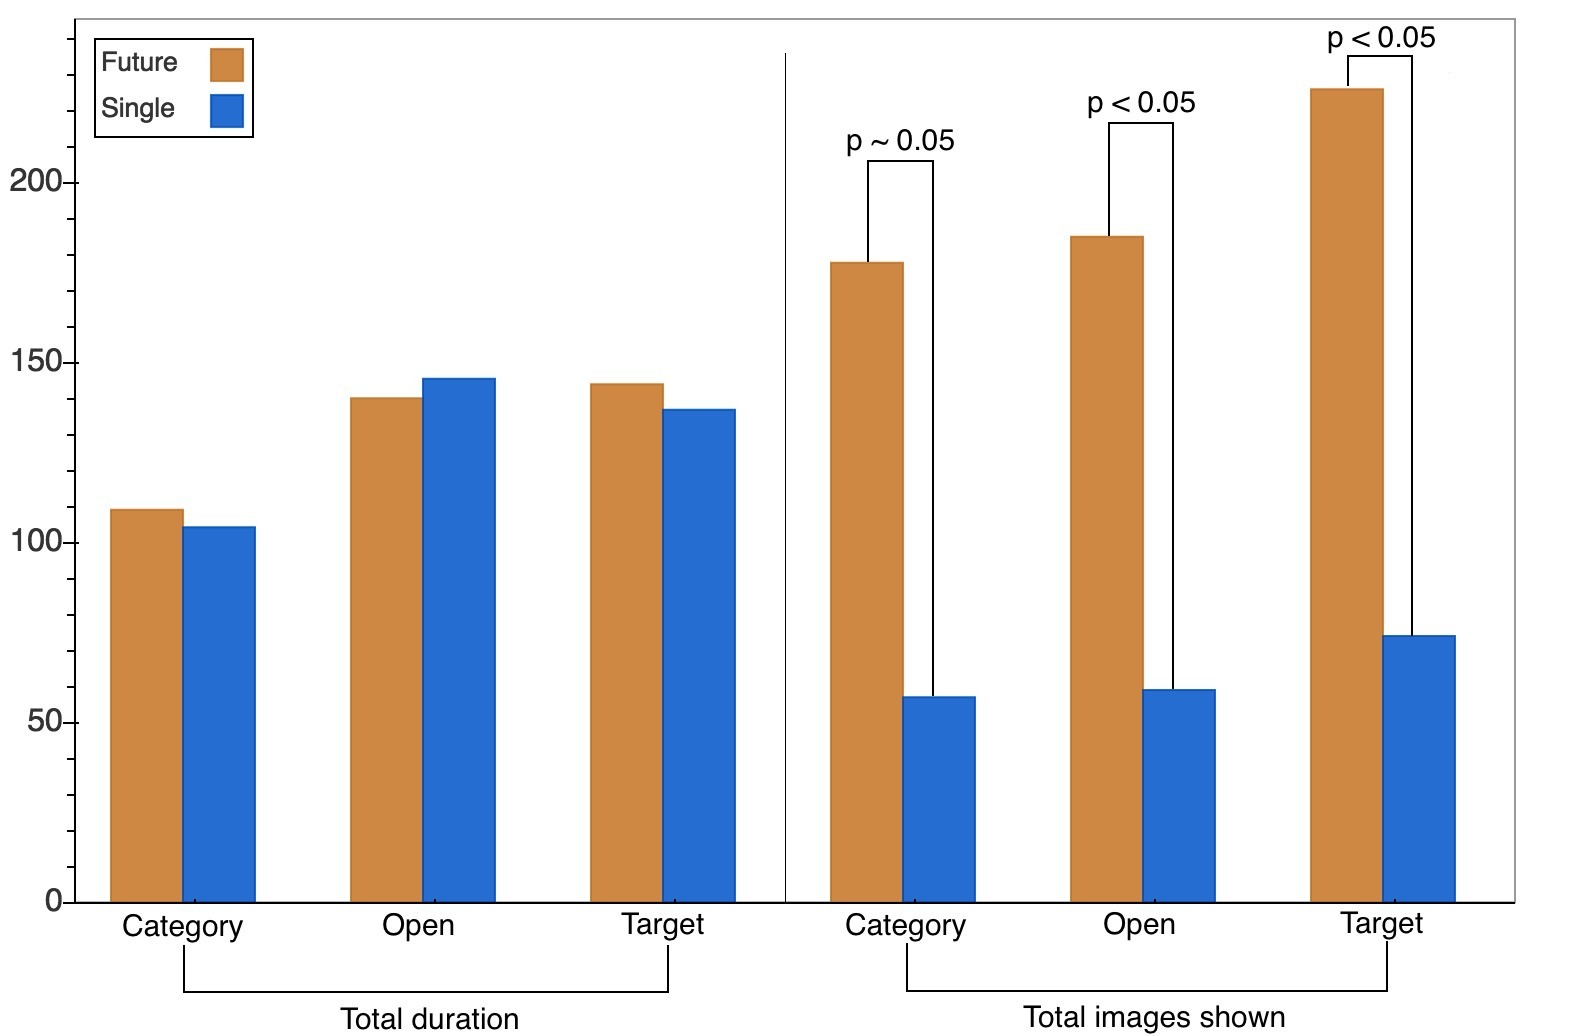
\includegraphics[width=0.95\textwidth,height=8cm]{figures/Bar_Chart__Duration_vs_Images.jpg}
    \caption{Total duration vs number of shown images}
    
    \label{dur_vs_img}
\end{figure}

\begin{table}
	
	\begin{center}
	\scalebox{0.65}{
    \begin{tabular}{|l|r|r|r|r|r|r|}
        \hline
        \multicolumn{7}{|c|}{\textbf{Genre wise Mean (Standard Deviation)}} \\
        \hline
        
        \multicolumn{1}{|c|}{} & \multicolumn{2}{|c|}{\textbf{Category}} & \multicolumn{2}{|c|}{\textbf{Open}} & \multicolumn{2}{|c|}{\textbf{Target}} \\
        \hline
        
        \multicolumn{1}{|c|}{} & \multicolumn{1}{|c|}{\textbf{Future}} & \multicolumn{1}{|c|}{\textbf{Single}} & \multicolumn{1}{|c|}{\textbf{Future}} & \multicolumn{1}{|c|}{\textbf{Single}} & \multicolumn{1}{|c|}{\textbf{Future}} & \multicolumn{1}{|c|}{\textbf{Single}} \\
        \hline
        
        \multicolumn{1}{|l|}{\textbf{Iterations}} & 14.83 (17.96) & 4.75 (4.75) & 15.42 (10.23) & 4.92 (4.48) & 18.83 (14.36) & 6.17 (4.71) \\
        \hline
        
        \multicolumn{1}{|l|}{\textbf{Avg. duration/Iteration (in Sec.)}} & 8.86 (2.96) & 24.39 (4.41) & 10.04 (4.06) & 31.26 (10.83) & 8.71 (2.8) & 24.44 (11.55) \\
        \hline
        
        \multicolumn{1}{|l|}{\textbf{Total duration (in Sec.)}} & 109.08 (101.72) & 104.25 (101.11) & 140.08 (84.13) & 145.5 (123.42) & 144 (95.11) & 136.92 (105.33) \\
        \hline
        
        \multicolumn{1}{|l|}{\textbf{Total shown images}} & 178 (215.57) & 57 (57.01) & 185 (122.75) & 59 (53.78) & 226 (172.37) & 74 (56.48) \\
        \hline
        
        \multicolumn{1}{|l|}{\textbf{Total feedback received}} & 14.83 (17.96) & 9.33 (8.05) & 15.42 (10.23) & 17.5 (18.26) & 18.83 (14.36) & 15.58 (17.68) \\
        \hline
        
    \end{tabular}
    }
	\end{center}
	\caption{Genre wise Mean and Standard Deviation of experiment parameters}
    \label{table:exp_mean_std_genre}
\end{table}

\iffalse
% Genre wise standard deviation of experiment parameters

\begin{table}
	\small
	\begin{center}
    \begin{tabular}{|l|r|r|r|r|r|r|}
        \hline
        \multicolumn{7}{|c|}{\textbf{Genre wise Standard Deviation}} \\
        \hline
        
        \multicolumn{1}{|c|}{} & \multicolumn{2}{|c|}{\textbf{Category}} & \multicolumn{2}{|c|}{\textbf{Open}} & \multicolumn{2}{|c|}{\textbf{Target}} \\
        \hline
        
        \multicolumn{1}{|c|}{} & \multicolumn{1}{|c|}{\textbf{Future}} & \multicolumn{1}{|c|}{\textbf{Single}} & \multicolumn{1}{|c|}{\textbf{Future}} & \multicolumn{1}{|c|}{\textbf{Single}} & \multicolumn{1}{|c|}{\textbf{Future}} & \multicolumn{1}{|c|}{\textbf{Single}} \\
        \hline
        
        \multicolumn{1}{|l|}{\textbf{Iterations}} & 17.96 & 4.75 & 10.23 & 4.48 & 14.36 & 4.71 \\
        \hline
        
        \multicolumn{1}{|l|}{\textbf{Avg. duration/Iteration (in Sec.)}} & 2.96 & 4.41 & 4.06 & 10.83 & 2.8 & 11.55 \\
        \hline
        
        \multicolumn{1}{|l|}{\textbf{Total duration (in Sec.)}} & 101.72 & 101.11 & 84.13 & 123.42 & 95.11 & 105.33 \\
        \hline
        
        \multicolumn{1}{|l|}{\textbf{Total shown images}} & 215.57 & 57.01 & 122.75 & 53.78 & 172.37 & 56.48 \\
        \hline
        
        \multicolumn{1}{|l|}{\textbf{Total feedback received}} & 17.96 & 8.05 & 10.23 & 18.26 & 14.36 & 17.68 \\
        \hline
        
    \end{tabular}
	\end{center}
	\caption{Genre wise Standard Deviation of experiment parameters}
    \label{table:exp_std_genre}
\end{table}

\fi

% Genre wise Wilcoxon P value (FutureView vs Single View) of experiment parameters

\begin{table}
	\small
	\begin{center}
    \begin{tabular}{|l|r|r|r|}
        \hline
        \multicolumn{4}{|c|}{\textbf{Genre wise Wilcoxon P value}} \\
        \hline
        
        \multicolumn{1}{|c|}{} & \multicolumn{1}{|c|}{\textbf{Category}} & \multicolumn{1}{|c|}{\textbf{Open}} & \multicolumn{1}{|c|}{\textbf{Target}} \\
        \hline
        
        
        
        \multicolumn{1}{|l|}{\textbf{Iterations}} & 0.05405584757 & 0.003239921272 & 0.0206095954 \\
        \hline
        
        \multicolumn{1}{|l|}{\textbf{Avg. duration/Iteration (in Sec.)}} & 0.002217721464 & 0.002217721464 & 0.002217721464 \\
        \hline
        
        \multicolumn{1}{|l|}{\textbf{Total duration (in Sec.)}} & 0.8139453463 & 0.9687003809 & 0.6378701799 \\
        \hline
        
        \multicolumn{1}{|l|}{\textbf{Total shown images}} & 0.05405584757 & 0.003239921272 & 0.0206095954 \\
        \hline
        
        \multicolumn{1}{|l|}{\textbf{Total feedback received}} & 0.7891658874 & 0.7555407781 & 0.3461504513 \\
        \hline
        
    \end{tabular}
	\end{center}
	\caption{Genre wise Wilcoxon P value measure of experiment parameters (FutureView vs Single View)}
    \label{table:exp_wilcoxon_genre}
\end{table}

 In Table \ref{table:exp_mean_std_task} and \ref{table:exp_wilcox_task} we show the task wise break up of the experiment parameters, respectively. From Table \ref{table:exp_wilcox_task} we see that the total number of shown images is significantly higher in FutureView for "city by night", "gardening", "happiness" and "tall building". Though for "red rose" and "seashore" it did not pass the threshold of statistical significance (p < 0.05). It happens because maybe the user found the desired image quickly in FutureView before terminating the search, resulting a limited number of shown images. On the other hand, in the single view may be the system explored a lot due to the presence of various colours in the images rated by the user, resulting a lot of iterations. Especially for "red rose" it is possible because the surrounding of a red rose can have multiple colours based on where it is. From Table \ref{table:exp_mean_std_task} we see that the mean total shown images is much higher in FutureView for those two tasks thus resulting a cumulative higher number overall for each genre.

% Task wise mean of experiment parameters

\begin{table}
	
	\begin{center}
	\scalebox{0.62}{
    \begin{tabular}{|l|r|r|r|r|r|r|}
        \hline
        \multicolumn{7}{|c|}{\textbf{Task wise Mean (Standard Deviation)}} \\
        \hline
        
        \multicolumn{1}{|c|}{} & \multicolumn{2}{|c|}{\textbf{City by Night}} & \multicolumn{2}{|c|}{\textbf{Gardening}} & \multicolumn{2}{|c|}{\textbf{Happiness}} \\
        \hline
        
        \multicolumn{1}{|c|}{} & \multicolumn{1}{|c|}{\textbf{Future}} & \multicolumn{1}{|c|}{\textbf{Single}} & \multicolumn{1}{|c|}{\textbf{Future}} & \multicolumn{1}{|c|}{\textbf{Single}} & \multicolumn{1}{|c|}{\textbf{Future}} & \multicolumn{1}{|c|}{\textbf{Single}} \\
        \hline
        
        \multicolumn{1}{|l|}{\textbf{Iterations}} & 8.33 (5.05) & 2.5  (2.35) & 16.33 (8.45) & 7 (5.76) & 14.50 (12.52) & 2.83 (0.75) \\
        \hline
        
        \multicolumn{1}{|l|}{\textbf{Avg. duration/Iteration (in Sec.)}} & 9.87 (3.5) & 24.7 (5.02) & 8.83 (2.58) & 31.24 (11.17) & 11.25 (5.1) & 31.27 (11.55) \\
        \hline
        
        \multicolumn{1}{|l|}{\textbf{Total duration (in Sec.)}} & 82.83 (58.99) & 54.17 (42.75) & 136.83 (74.83) & 209 (153.56) & 143.33 (99.73) & 82 (15.89) \\
        \hline
        
        \multicolumn{1}{|l|}{\textbf{Total shown images}} & 100 (60.56) & 30 (28.14) & 196 (101.45) & 84 (69.14) & 174 (150.22) & 34 (9.03) \\
        \hline
        
        \multicolumn{1}{|l|}{\textbf{Total feedback received}} & 8.33 (5.05) & 4.67 (3.56) & 16.33 (8.45) & 25.5 (23.97) & 14.5  (12.52) & 9.5 (2.35) \\
        \hline
        \hline
        \multicolumn{1}{|c|}{} & \multicolumn{2}{|c|}{\textbf{Red Rose}} & \multicolumn{2}{|c|}{\textbf{Seashore}} & \multicolumn{2}{|c|}{\textbf{Tall Building}} \\
        \hline
        
        \multicolumn{1}{|c|}{} & \multicolumn{1}{|c|}{\textbf{Future}} & \multicolumn{1}{|c|}{\textbf{Single}} & \multicolumn{1}{|c|}{\textbf{Future}} & \multicolumn{1}{|c|}{\textbf{Single}} & \multicolumn{1}{|c|}{\textbf{Future}} & \multicolumn{1}{|c|}{\textbf{Single}} \\
        \hline
        
        \multicolumn{1}{|l|}{\textbf{Iterations}} & 23.83 (18.17) & 7.67 (6.09) & 21.33 (24.15) & 7 (5.66) & 13.83 (7.99) & 4.67 (2.5) \\
        \hline
        
        \multicolumn{1}{|l|}{\textbf{Avg. duration/Iteration (in Sec.)}} & 9.04 (3.67) & 20.58 (2.8) & 7.84 (2.13) & 24.09  (4.18) & 8.37 (1.87) & 28.3 (15.81) \\
        \hline
        
        \multicolumn{1}{|l|}{\textbf{Total duration (in Sec.)}} & 169.5 (112.02) & 157 (137.22) & 135.33 (132.78) & 154.33 (121.01) & 118.5 (76.11) & 116.83 (67.91) \\
        \hline
        
        \multicolumn{1}{|l|}{\textbf{Total shown images}} & 286 (218.05) & 92 (73.06) & 256 (289.76) & 84 (67.88) & 166 (95.82) & 56 (30.04) \\
        \hline
        
        \multicolumn{1}{|l|}{\textbf{Total feedback received}} & 23.83 (18.17) & 22.33 (23.37) & 21.33 (24.15) & 14 (8.81) & 13.83 (7.99) & 8.83 (5.67) \\
        \hline

    \end{tabular}
    }
	\end{center}
	\caption{Task wise Mean and Standard Deviation of experiment parameters}
    \label{table:exp_mean_std_task}
\end{table}


\iffalse
% Task wise standard deviation of experiment parameters

\begin{table}
	\small
	\begin{center}
    \begin{tabular}{|l|r|r|r|r|r|r|}
        \hline
        \multicolumn{7}{|c|}{\textbf{Task wise Standard Deviation}} \\
        \hline
        
        \multicolumn{1}{|c|}{} & \multicolumn{2}{|c|}{\textbf{City by Night}} & \multicolumn{2}{|c|}{\textbf{Gardening}} & \multicolumn{2}{|c|}{\textbf{Happiness}} \\
        \hline
        
        \multicolumn{1}{|c|}{} & \multicolumn{1}{|c|}{\textbf{Future}} & \multicolumn{1}{|c|}{\textbf{Single}} & \multicolumn{1}{|c|}{\textbf{Future}} & \multicolumn{1}{|c|}{\textbf{Single}} & \multicolumn{1}{|c|}{\textbf{Future}} & \multicolumn{1}{|c|}{\textbf{Single}} \\
        \hline
        
        \multicolumn{1}{|l|}{\textbf{Iterations}} & 5.05 & 2.35 & 8.45 & 5.76 & 12.52 & 0.75 \\
        \hline
        
        \multicolumn{1}{|l|}{\textbf{Avg. duration/Iteration (in Sec.)}} & 3.5 & 5.02 & 2.58 & 11.17 & 5.1 & 11.55 \\
        \hline
        
        \multicolumn{1}{|l|}{\textbf{Total duration (in Sec.)}} & 58.99 & 42.75 & 74.83 & 153.56 & 99.73 & 15.89 \\
        \hline
        
        \multicolumn{1}{|l|}{\textbf{Total shown images}} & 60.56 & 28.14 & 101.45 & 69.14 & 150.22 & 9.03 \\
        \hline
        
        \multicolumn{1}{|l|}{\textbf{Total feedback received}} & 5.05 & 3.56 & 8.45 & 23.97 & 12.52 & 2.35 \\
        \hline
        \hline
        \multicolumn{1}{|c|}{} & \multicolumn{2}{|c|}{\textbf{Red Rose}} & \multicolumn{2}{|c|}{\textbf{Seashore}} & \multicolumn{2}{|c|}{\textbf{Tall Building}} \\
        \hline
        
        \multicolumn{1}{|c|}{} & \multicolumn{1}{|c|}{\textbf{Future}} & \multicolumn{1}{|c|}{\textbf{Single}} & \multicolumn{1}{|c|}{\textbf{Future}} & \multicolumn{1}{|c|}{\textbf{Single}} & \multicolumn{1}{|c|}{\textbf{Future}} & \multicolumn{1}{|c|}{\textbf{Single}} \\
        \hline
        
        \multicolumn{1}{|l|}{\textbf{Iterations}} & 18.17 & 6.09 & 24.15 & 5.66 & 7.99 & 2.5 \\
        \hline
        
        \multicolumn{1}{|l|}{\textbf{Avg. duration/Iteration (in Sec.)}} & 3.67 & 2.8 & 2.13 & 4.18 & 1.87 & 15.81 \\
        \hline
        
        \multicolumn{1}{|l|}{\textbf{Total duration (in Sec.)}} & 112.02 & 137.22 & 132.78 & 121.01 & 76.11 & 67.91 \\
        \hline
        
        \multicolumn{1}{|l|}{\textbf{Total shown images}} & 218.05 & 73.06 & 289.76 & 67.88 & 95.82 & 30.04 \\
        \hline
        
        \multicolumn{1}{|l|}{\textbf{Total feedback received}} & 18.17 & 23.37 & 24.15 & 8.81 & 7.99 & 5.67 \\
        \hline

    \end{tabular}
	\end{center}
	\caption{Task wise Standard Deviation of experiment parameters}
    \label{table:exp_std_task}
\end{table}
\fi
% Task wise Wilcoxon P value (FutureView vs Single View) of experiment parameters

\begin{table}
	\small
	\begin{center}
    \begin{tabular}{|l|r|r|r|}
        \hline
        \multicolumn{4}{|c|}{\textbf{Task wise Wilcoxon P value}} \\
        \hline
        
        
        
        \multicolumn{1}{|c|}{} & \multicolumn{1}{|c|}{\textbf{City by Night}} & \multicolumn{1}{|c|}{\textbf{Gardening}} & \multicolumn{1}{|c|}{\textbf{Happiness}} \\
        \hline
        
        \multicolumn{1}{|l|}{\textbf{Iterations}} & 0.07473549831 & 0.02770784936 & 0.02770784936 \\
        \hline
        
        \multicolumn{1}{|l|}{\textbf{Avg. duration/Iteration (in Sec.)}} & 0.02770784936 & 0.02770784936 & 0.04639946187 \\
        \hline
        
        \multicolumn{1}{|l|}{\textbf{Total duration (in Sec.)}} & 0.3454475305 & 0.3454475305 & 0.172954918 \\
        \hline
        
        \multicolumn{1}{|l|}{\textbf{Total shown images}} & 0.07473549831 & 0.02770784936 & 0.02770784936 \\
        \hline
        
        \multicolumn{1}{|l|}{\textbf{Total feedback received}} & 0.2071604489 & 0.3454475305 & 0.5282327769 \\
        \hline
        \hline
        
        \multicolumn{1}{|c|}{} & \multicolumn{1}{|c|}{\textbf{Red Rose}} & \multicolumn{1}{|c|}{\textbf{Seashore}} & \multicolumn{1}{|c|}{\textbf{Tall Building}} \\
        \hline
		
		\multicolumn{1}{|l|}{\textbf{Iterations}} & 0.172954918 & 0.1380107376 & 0.02728117148 \\
        \hline
        
        \multicolumn{1}{|l|}{\textbf{Avg. duration/Iteration (in Sec.)}} & 0.02770784936 & 0.02770784936 & 0.02770784936 \\
        \hline
        
        \multicolumn{1}{|l|}{\textbf{Total duration (in Sec.)}} & 0.6001794871 & 0.6001794871 & 0.9165119079 \\
        \hline
        
        \multicolumn{1}{|l|}{\textbf{Total shown images}} & 0.172954918 & 0.1380107376 & 0.02728117148 \\
        \hline
        
        \multicolumn{1}{|l|}{\textbf{Total feedback received}} & 0.5001842571 & 0.752493649 & 0.1380107376 \\
        \hline
        
    \end{tabular}
	\end{center}
	\caption{Task wise Wilcoxon P value measure of experiment parameters (FutureView vs Single View)}
    \label{table:exp_wilcox_task}
\end{table}

We also calculated the aggregates on usability parameters extracted from the NASA  TLX questionnaire the users had to fill up after every task ended. These parameters were rated on a scale from 1 to 10. From Table \ref{table:use_mean_std_genre} we see that for all the genres, the users felt more successful in the FutureView. It also shows that the amount of hard work needed to finish the tasks were more in single view in category search and target search. For open ended search it went otherwise. The reason could be that as the nature of the task did not give any fixed target, the users were diverted a bit when they were exposed to more exploration and could not frame a proper target in some cases thus explored a lot more than required. From Table \ref{table:use_wilcoxon_genre} we see that for open ended search, the fact that the users felt more successful in accomplishing the tasks in FutureView, is statistically significant. Figure \ref{fig:bar_chart_NASA_TLX} shows a summary of the usability parameters.


\begin{figure}[h!]
  \centering
    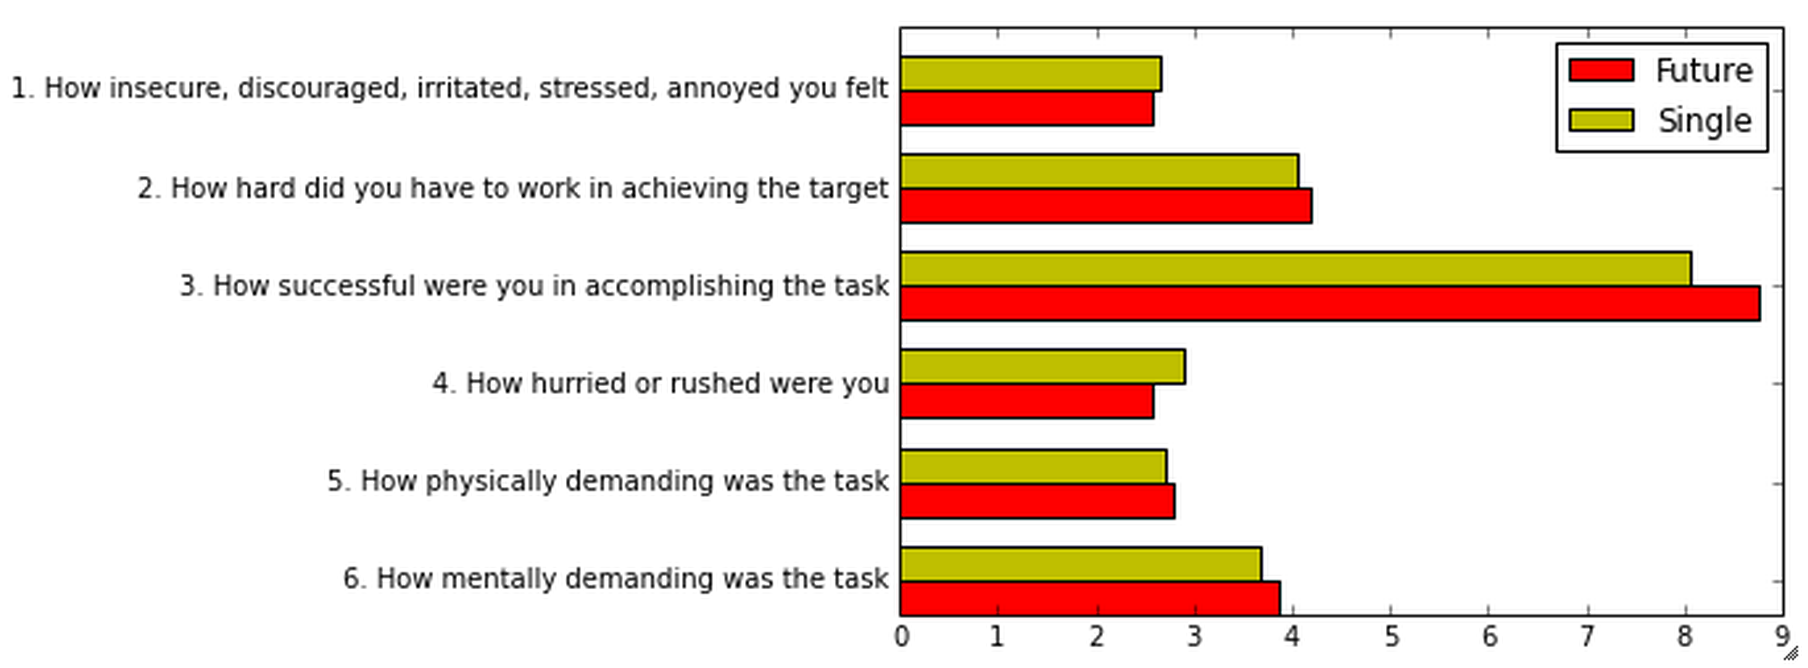
\includegraphics[width=1.0\textwidth,height=7cm]{figures/Bar_chart_usability_parameters_numbered.png}
    \caption{Comparison of usability parameters according to NASA TLX}
    \label{fig:bar_chart_NASA_TLX}
\end{figure}


% Genre wise Mean of usability parameters

\begin{table}
	
	\begin{center}
	\scalebox{0.7}{
    \begin{tabular}{|p{6cm}|r|r|r|r|r|r|}
        \hline
        \multicolumn{7}{|c|}{\textbf{Genre wise Mean (Standard Deviation)}} \\
        \hline
        
        \multicolumn{1}{|c|}{} & \multicolumn{2}{|c|}{\textbf{Category}} & \multicolumn{2}{|c|}{\textbf{Open}} & \multicolumn{2}{|c|}{\textbf{Target}} \\
        \hline
        
        \multicolumn{1}{|c|}{} & \multicolumn{1}{|c|}{\textbf{Future}} & \multicolumn{1}{|c|}{\textbf{Single}} & \multicolumn{1}{|c|}{\textbf{Future}} & \multicolumn{1}{|c|}{\textbf{Single}} & \multicolumn{1}{|c|}{\textbf{Future}} & \multicolumn{1}{|c|}{\textbf{Single}} \\
        \hline
        
        \textbf{How mentally demanding was the task?} & 3.42 (2.27) & 3 (1.6) & 4.42 (2.23) & 4.08 (1.73) & 3.75 (1.66) & 3.92 (1.78) \\
        \hline
        
        \textbf{How physically demanding was the task?} & 2.75 (2.6) & 2.5 (1.88) & 2.67 (2.15) & 2.67 (1.61) & 2.92 (2.07) & 3 (1.81) \\
        \hline
        
        \textbf{How hurried or rushed you felt while performing the task?} & 2.75 (1.82) & 2.67 (1.56) & 2.75 (1.48) & 3 (1.81) & 2.25 (1.42) & 3 (1.95) \\
        \hline
        
        \textbf{How successful were you in accomplishing the task?} & 9.08 (1.68) & 8.67 (1.3) & 8.83 (1.11) & 7.83 (1.27) & 8.33 (1.61) & 7.67 (2.57) \\
        \hline
        
        \textbf{How hard did you have to work for accomplishing the task?} & 3.58 (2.61) & 3.83 (2.33) & 5.33 (2.67) & 4.42 (2.35) & 3.67 (1.83) & 3.92 (2.15) \\
        \hline
        
        \textbf{How insecure, discouraged, irritated, stressed and annoyed were you?} & 2.33 (2.1) & 2.08 (1.16) & 3 (2.45) & 3.08 (1.68) & 2.42 (1.73) & 2.83 (2.21) \\
        \hline
        
    \end{tabular}
    }
	\end{center}
	\caption{Genre wise Mean and Standard Deviation of usability parameters according to NASA TLX questionnaire}
    \label{table:use_mean_std_genre}
\end{table}

\iffalse

% Genre wise STD of usability parameters

\begin{table}
	\small
	\begin{center}
    \begin{tabular}{|p{6cm}|r|r|r|r|r|r|}
        \hline
        \multicolumn{7}{|c|}{\textbf{Genre wise Standard Deviation}} \\
        \hline
        
        \multicolumn{1}{|c|}{} & \multicolumn{2}{|c|}{\textbf{Category}} & \multicolumn{2}{|c|}{\textbf{Open}} & \multicolumn{2}{|c|}{\textbf{Target}} \\
        \hline
        
        \multicolumn{1}{|c|}{} & \multicolumn{1}{|c|}{\textbf{Future}} & \multicolumn{1}{|c|}{\textbf{Single}} & \multicolumn{1}{|c|}{\textbf{Future}} & \multicolumn{1}{|c|}{\textbf{Single}} & \multicolumn{1}{|c|}{\textbf{Future}} & \multicolumn{1}{|c|}{\textbf{Single}} \\
        \hline
        
        \textbf{How mentally demanding was the task?} & 2.27 & 1.6 & 2.23 & 1.73 & 1.66 & 1.78 \\
        \hline
        
        \textbf{How physically demanding was the task?} & 2.6 & 1.88 & 2.15 & 1.61 & 2.07 & 1.81 \\
        \hline
        
        \textbf{How hurried or rushed you felt while performing the task?} & 1.82 & 1.56 & 1.48 & 1.81 & 1.42 & 1.95 \\
        \hline
        
        \textbf{How successful were you in accomplishing the task?} & 1.68 & 1.3 & 1.11 & 1.27 & 1.61 & 2.57 \\
        \hline
        
        \textbf{How hard did you have to work for accomplishing the task?} & 2.61 & 2.33 & 2.67 & 2.35 & 1.83 & 2.15 \\
        \hline
        
        \textbf{How insecure, discouraged, irritated, stressed and annoyed were you?} & 2.1 & 1.16 & 2.45 & 1.68 & 1.73 & 2.21 \\
        \hline
        
    \end{tabular}
	\end{center}
	\caption{Genre wise Standard Deviation of usability parameters}
    \label{table:use_std_genre}
\end{table}

\fi

% Genre wise Wilcoxon P value (FutureView vs Single View) of usability parameters

\begin{table}
	\small
	\begin{center}
    \begin{tabular}{|p{6cm}|r|r|r|}
        \hline
        \multicolumn{4}{|c|}{\textbf{Genre wise Wilcoxon P value}} \\
        \hline
        
        \multicolumn{1}{|c|}{} & \multicolumn{1}{|c|}{\textbf{Category}} & \multicolumn{1}{|c|}{\textbf{Open}} & \multicolumn{1}{|c|}{\textbf{Target}} \\
        \hline
        
        
        
        \textbf{How mentally demanding was the task?} & 0.5817769166 & 0.8767217432 & 0.7957199701 \\
        \hline
        
        \textbf{How physically demanding was the task?} & 0.5879367462 & 1 & 0.7054569861 \\
        \hline
        
        \textbf{How hurried or rushed you felt while performing the task?} & 0.7301661743 & 0.5890107045 & 0.04734500209 \\
        \hline
        
        \textbf{How successful were you in accomplishing the task?} & 0.4982248534 & 0.02192029034 & 0.5124416997 \\
        \hline
        
        \textbf{How hard did you have to work for accomplishing the task?} & 0.6846218727 & 0.4126908569 & 0.8582145731 \\
        \hline
        
        \textbf{How insecure, discouraged, irritated, stressed and annoyed were you?} & 0.864324782 & 0.8772900143 & 0.6666320553 \\
        \hline
        
    \end{tabular}
	\end{center}
	\caption{Genre wise Wilcoxon P value measure of usability parameters according to NASA TLX questionnaire (FutureView vs Single View)}
    \label{table:use_wilcoxon_genre}
\end{table}

\begin{figure}[!h]
  \centering
    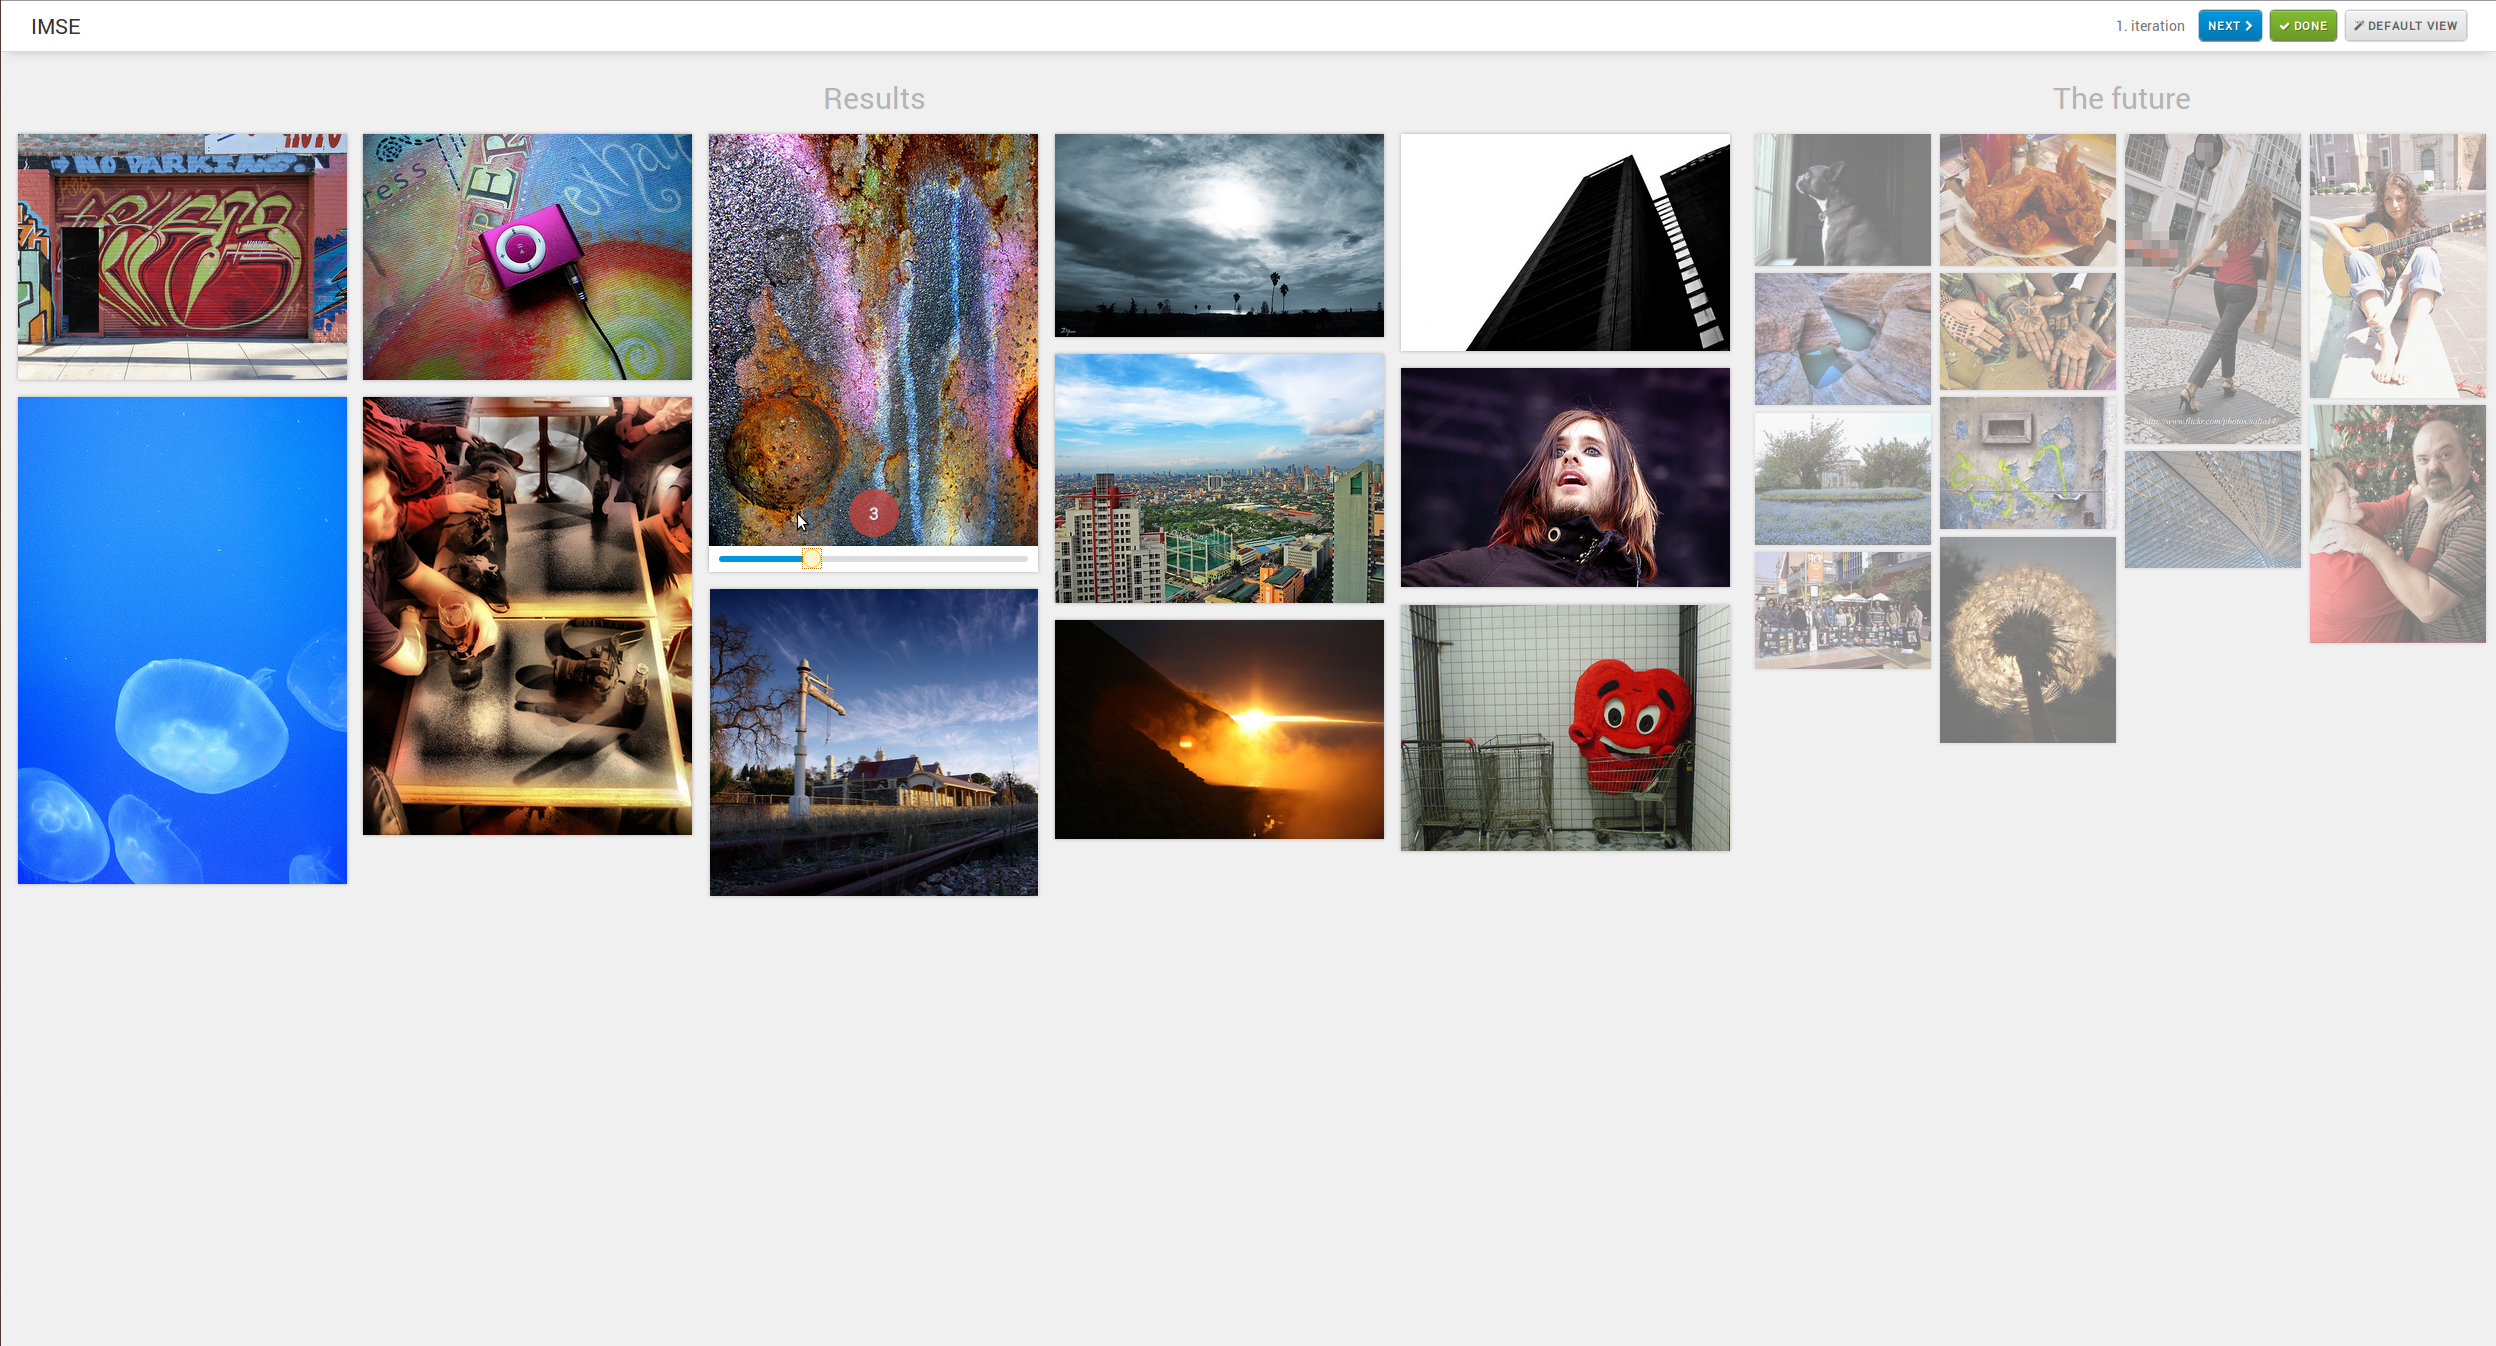
\includegraphics[width=0.90\textwidth,height=6cm]{figures/gardening_1.jpg}
    \caption{Gardening Iteration 1}
    \label{gardening_1}
\end{figure}

\begin{figure}[!h]
  \centering
    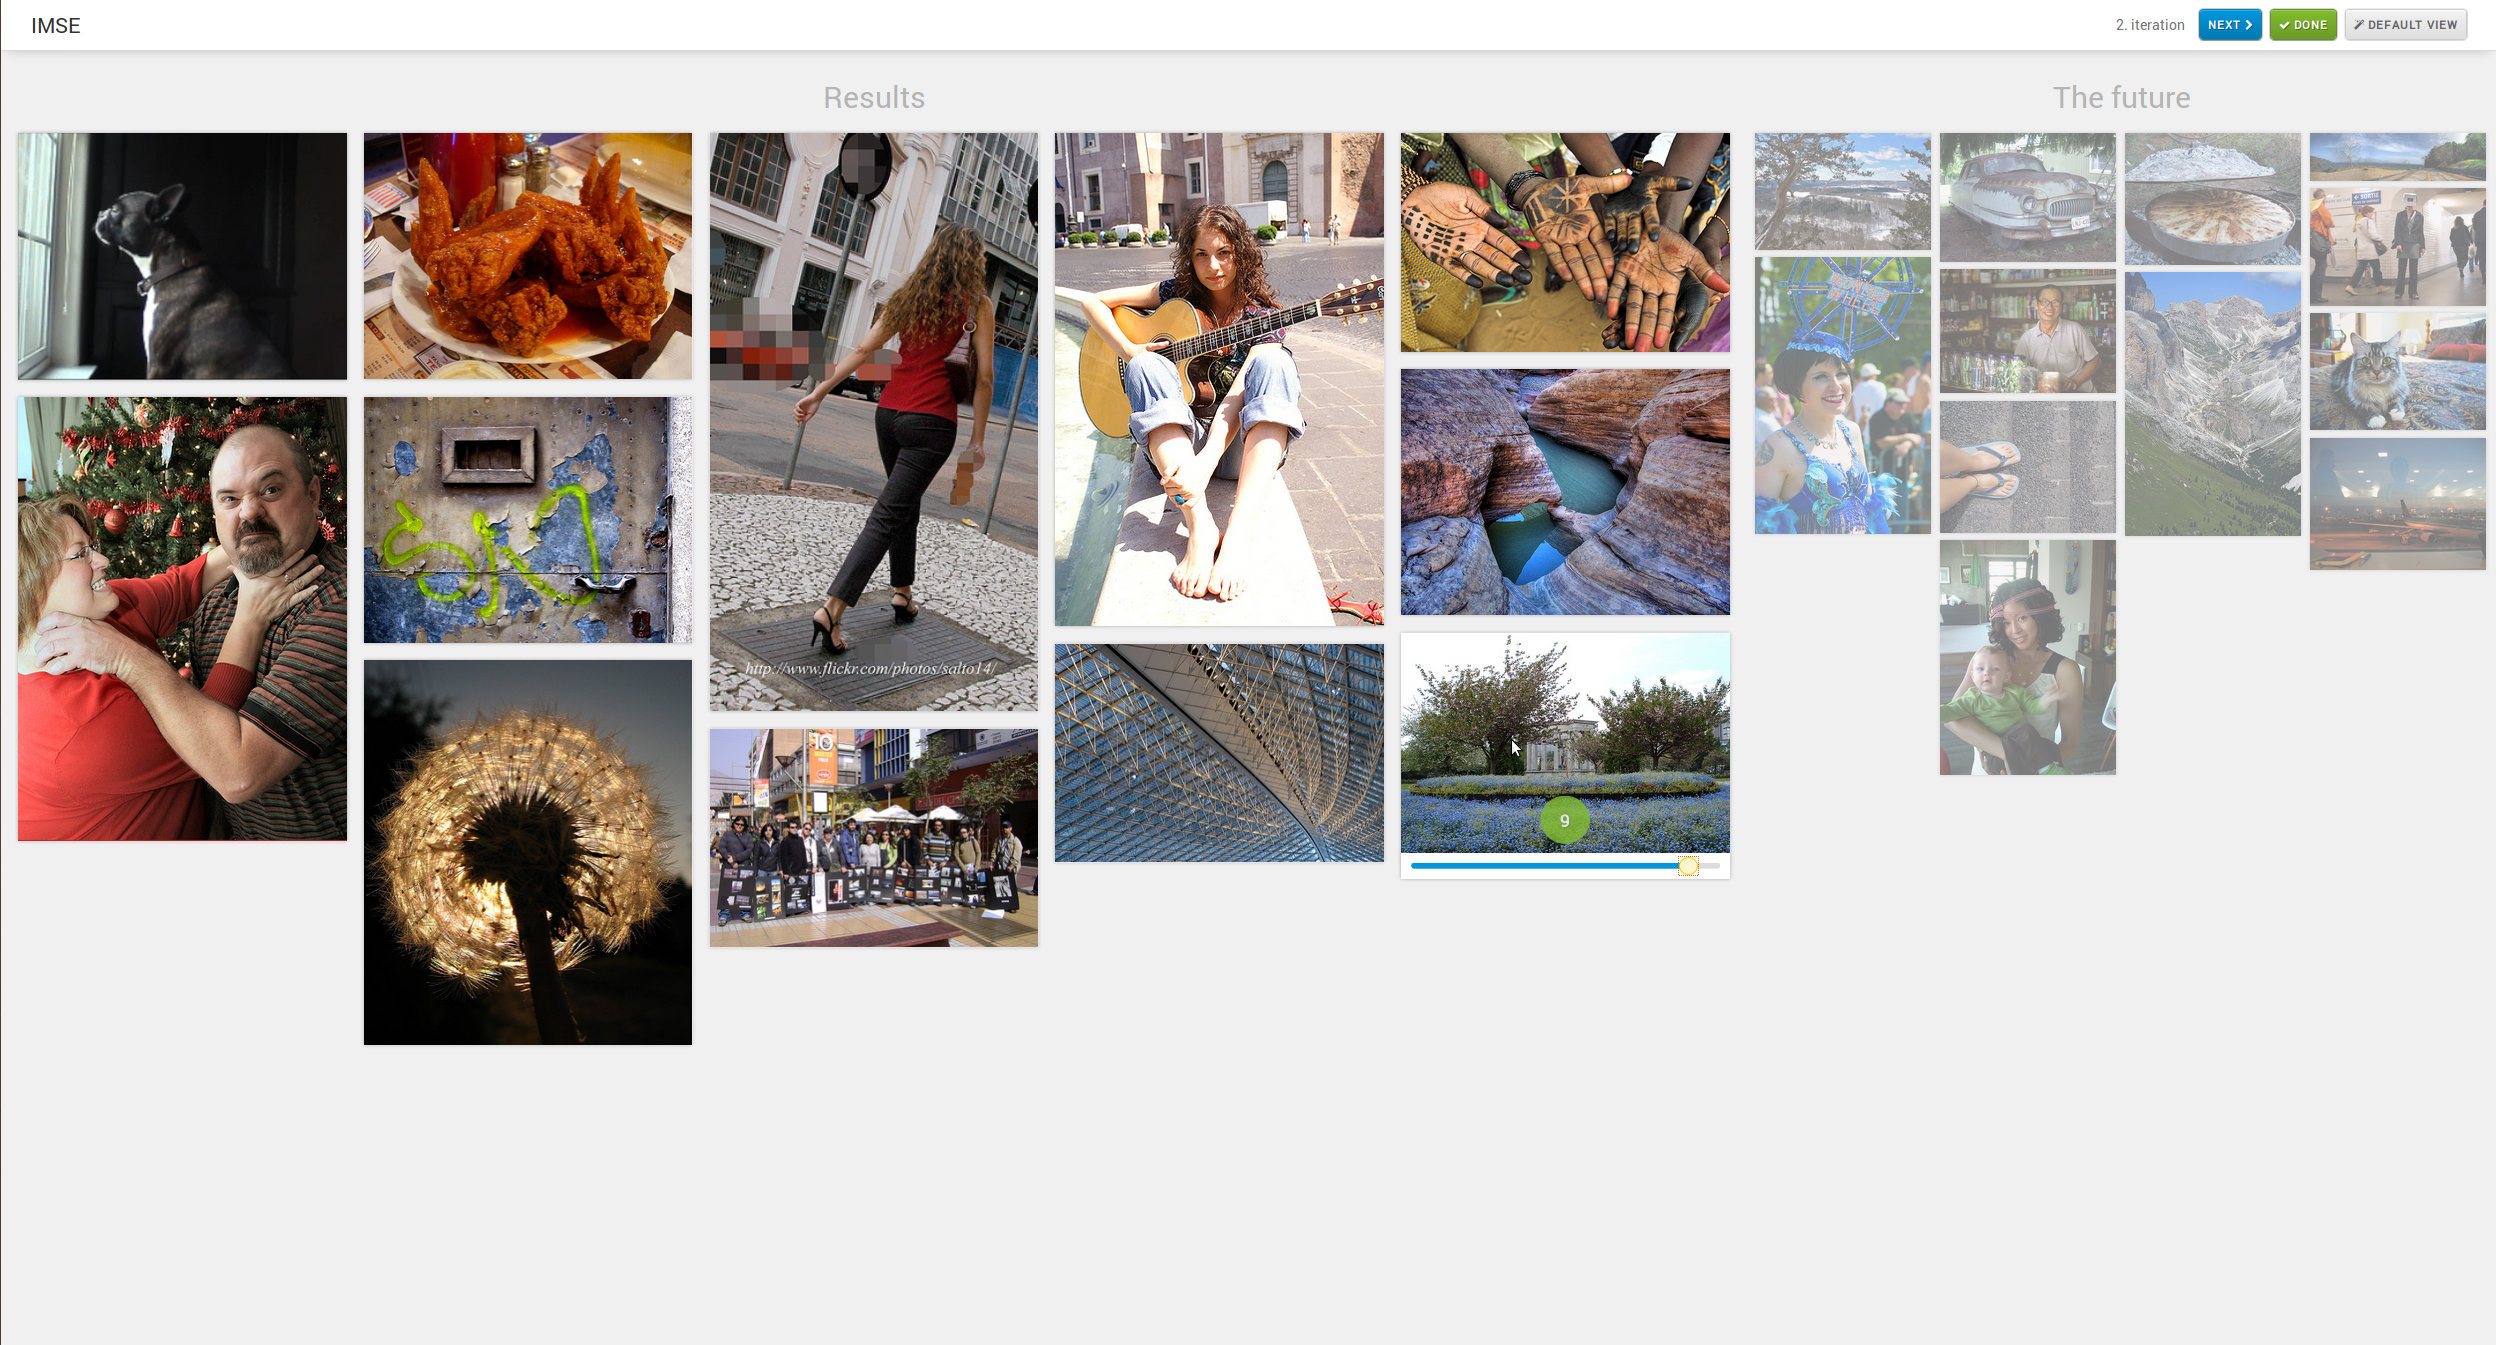
\includegraphics[width=0.90\textwidth,height=6cm]{figures/gardening_2.jpg}
    \caption{Gardening Iteration 2}
    \label{gardening_2}
\end{figure}

\begin{figure}[!h]
  \centering
    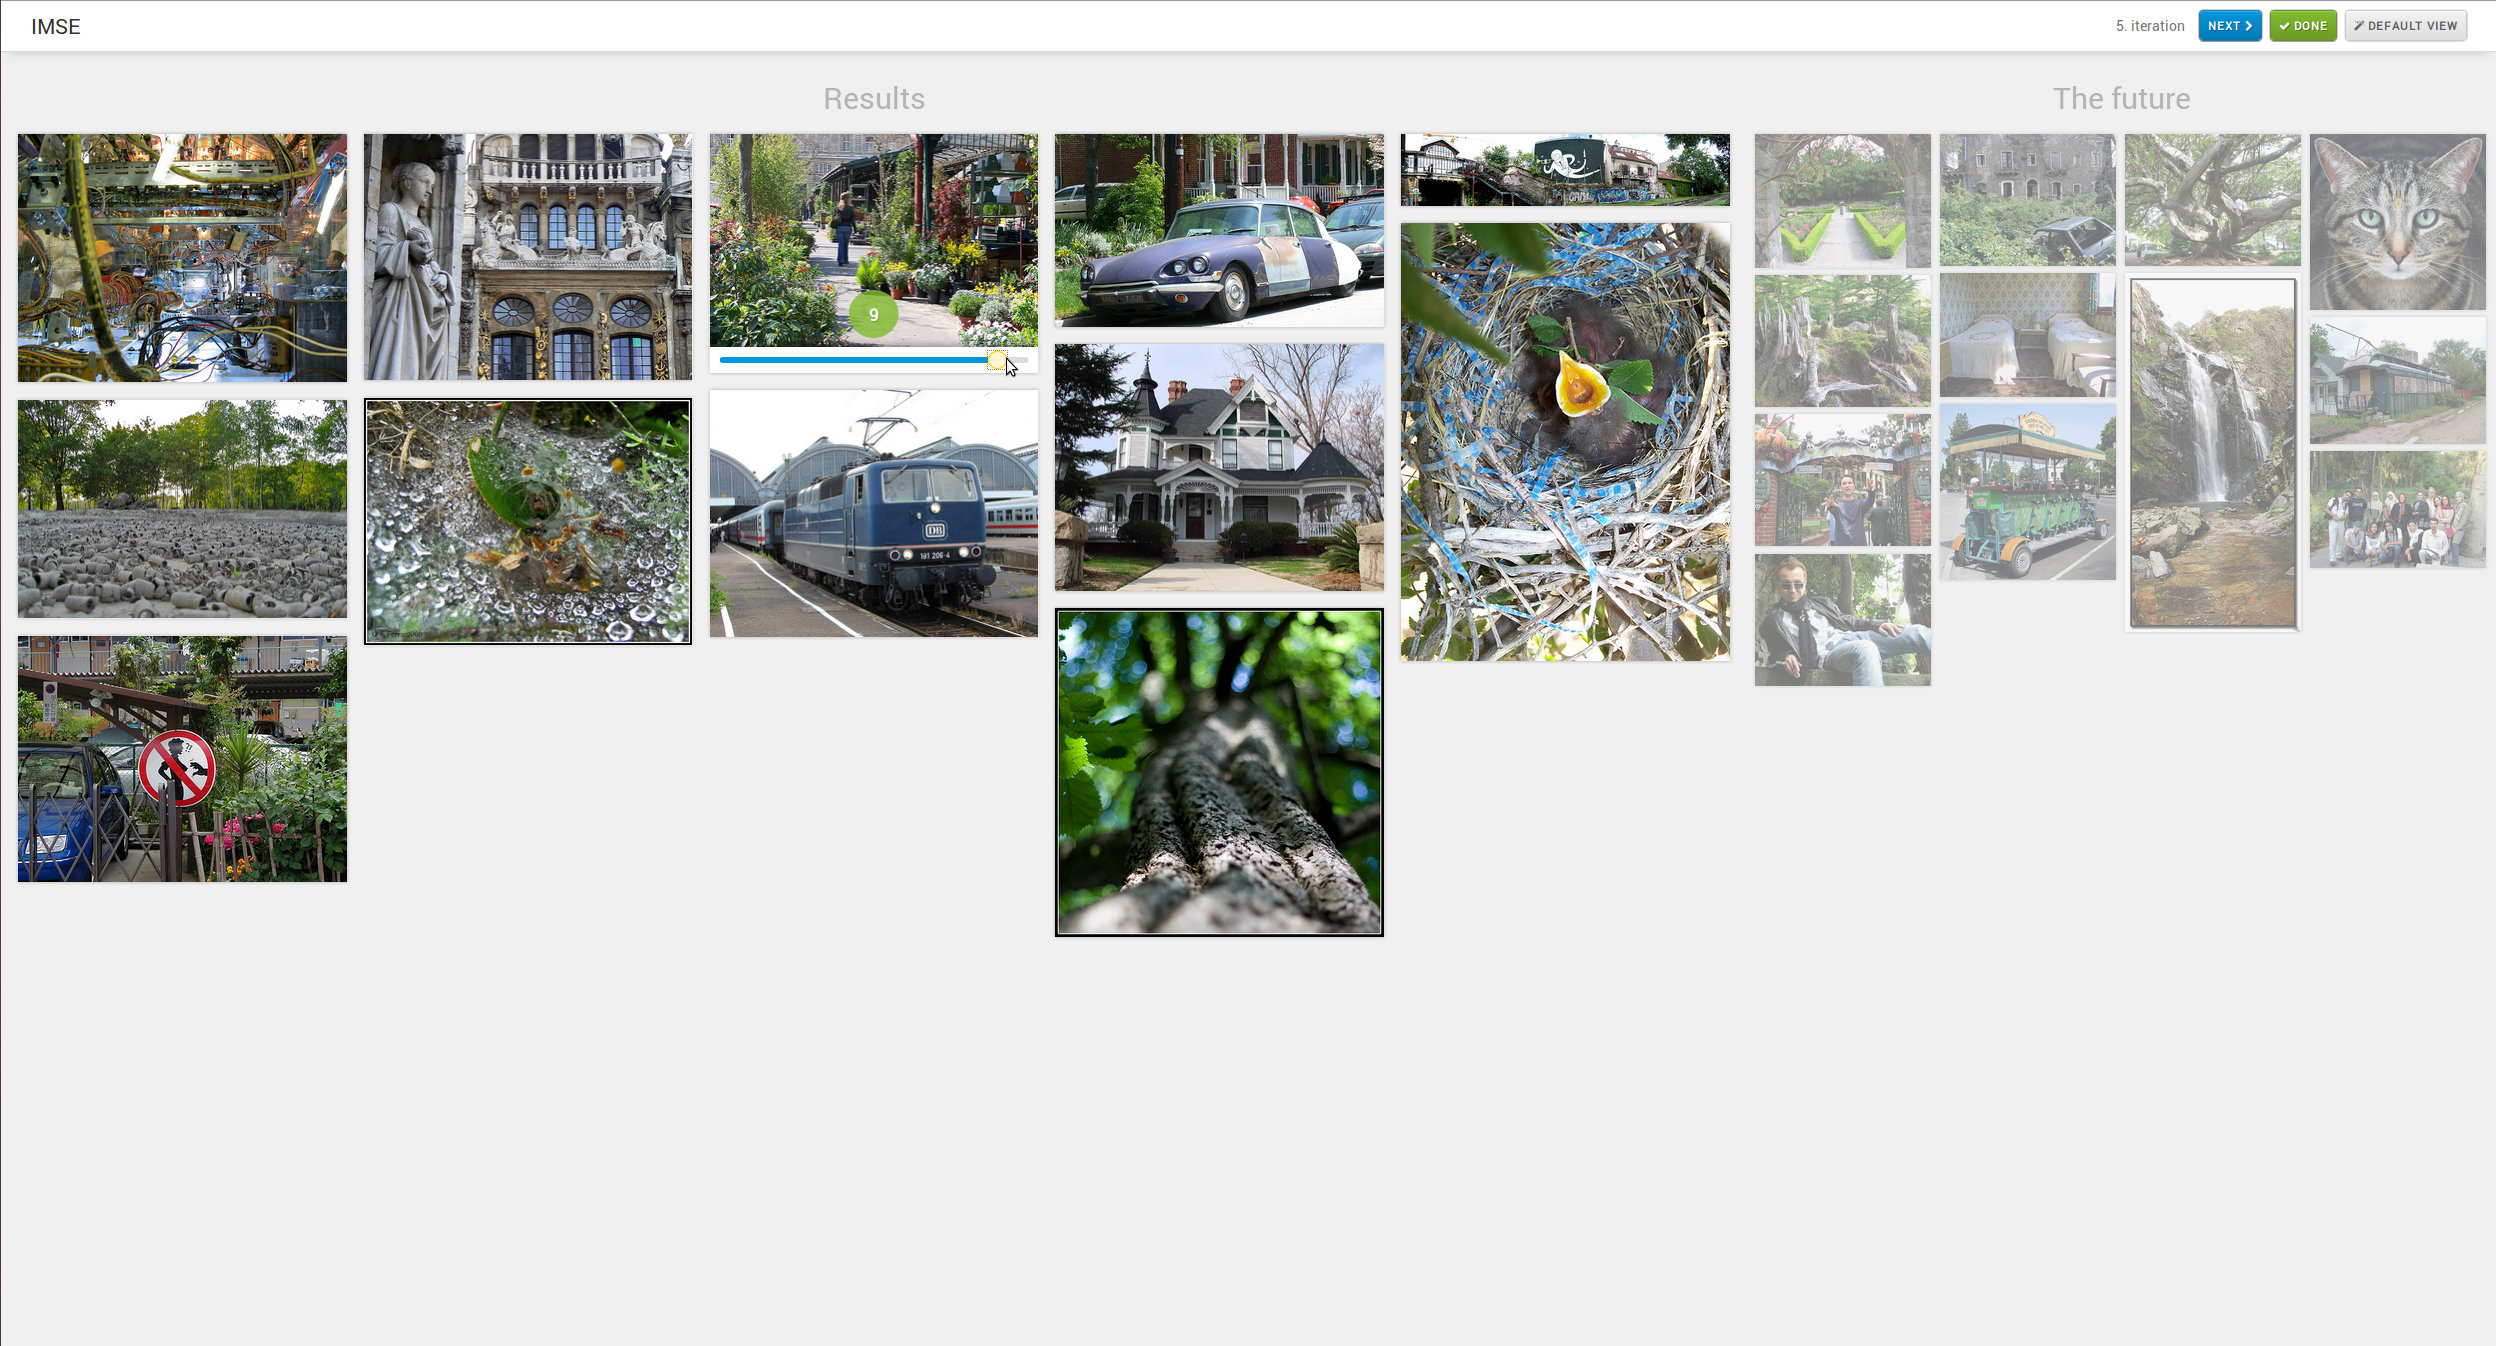
\includegraphics[width=0.90\textwidth,height=6cm]{figures/gardening_5.jpg}
    \caption{Gardening Iteration 5}
    \label{gardening_5}
\end{figure}

From Table \ref{table:use_mean_std_task} we see that for tasks "city by night", "gardening", "happiness", "red rose" and "seashore", users felt more successful in the FutureView, while only for "tall building" both the views performed equally good. The reason for this could be that all the tasks other than "tall building" involves various combination of colours. Say for "red rose", the user rates a picture of a red rose in a flower vase in a room or a red rose in a garden with other flowers or plants in the surroundings. In these two cases we have two different global colour spaces. As the system considers only colour from the entire image rated, the recommended images can be very different from each other in case of these two red roses. Therefore, the user had to adjust the ratings to get the desired images in FutureView while single view did not produce the actual images always. The same can be said for example for "city by night". An example image can consist a lot of cars on road, or a public gathering or a deserted street at midnight with a lot or a few street lights or lights from nearby buildings. We see here also based on the images rated, the next set of recommended images can vary a lot. While for "tall building", there is a very little space for variation. An image representing so should consist one or a few "tall buildings" under the sky. We do not expect a lot of variations in the colours of buildings (at least modern high rise buildings are not made multicoloured) and the sky, so, whatever image the user chooses, there cannot be a wild variation in the possible outcome, leaving not much space for adjustment in the FutureView. Figure \ref{gardening_1} and Figure \ref{gardening_2} shows the first two iterations of the experiment with task Gardening in FutureView. They show how the experiment started with images in random colour spaces even in FutureView and Figure \ref{gardening_5} shows how it converged to a green heavy colour space with a few relevant images in the last iteration.

\subsection{Excerpts from interviews}

The users liked the concept of FutureView overall and they talked about that in the interviews. They said some positive things about the FutureView, like, the FutureView helped them reaching their target image more quickly than the single view, they felt secure in the navigation more in the FutureView as they could see what images are getting picked up in each step, they did not see a live view before in any of the image search systems they have used before, the FutureView is more useful to people whose job includes searching for images. The last statement supports our goal to make a system that does not just search for discrete individual images, but helps building up a story or help reaching near a story step by step. It helps searching for images which are hard to describe in a finite combination of tags.

\section{Changes suggested}

The users were asked for suggestions for changes or modification to the system. They provided a few good suggestions as,

\begin{itemize}
	\item The system might include searching by text. We assume that as most image search systems include searching by text queries, the users felt that feature is missing but the system was not designed to accept text queries.
	\item The system does not track history. This was one of the major complains. When a user sees something interesting in the FutureView but still wants to explore a bit more, they demanded a way to save that instance like a checkpoint. Right now as the images are picked up randomly, if a user drags a slider and the images in the FutureView appear not so appealing and the user pushes the slider back to the previous state, the system does not get back to the exact same state, i.e. the system does not show the exact same set of images presented before dragging the slider. That is a major issue according to most of the users.
	\item The images in the FutureView were purposefully kept a bit blurred out so that the two views appear visually different. The users did not like it. They felt that because of that blurring they could not see the actual colour of the images in the FutureView thus in a few occasions could not decide whether they had received the image they were looking for. As the system relies on colour, it was a major drawback from the usability point of view.
\end{itemize}

\section{Problems with the system}

Apart from what the users suggested we also felt some issues with the system while running the study. They are,

\begin{itemize}
	\item The web server (Apache 2) needed to be restarted after each user finishes otherwise the system might crash. It crashed a couple of times resulting in a restart in the ongoing task. Actually, we show a lot of images which somehow clogs the browser or the memory in the backend. Restarting a server cannot be a solution. We should have a mechanism to clear images from previous experiments.
	\item The FutureView takes nearly a second to load. Sometimes users being too impatient, clicked on the next button right after dragging a slider without waiting for the FutureView to load. It led to a crash in the front end. We should disable the next button while the FutureView loads.
	\item One experiment had to be cancelled because a user used arrow keys on the keyboard to move the slider rather than dragging with mouse. We record mouse events to sync with eye tracker therefore arrow key press was useless. We should have had disabled those keys. 
\end{itemize}

\section{Future plan}

The study gave rise to a few questions and place for improvements which we will try to address in the next study.

\begin{itemize}
	\item One obvious place for improvement is to change the feedback system. Instead of dragging a tiny slider control, we can let the user rate the images quicker and with more convenience. This will bring the cognitive load down further.
	\item Enabling user to circle parts of images and let the system detect identifiable objects from the circled area and search for those objects is another area of research.
	\item Right now the system uses only colour as feature. We can put other features as texture, shape etc. and build separate kernels for them. We can then make the system search in all these different kernels and combine results from these multiple kernels in the end.
	\item The eye-tracker can be put to further use. We can record the implicit feedback from the eye-tracker and compare that with the actual recorded feedback to infer the mental state of the user. We can see how attentive they were during the experiment and whether they provided feedback keeping the task in mind or randomly.
\end{itemize}

\section{Conclusion}

The aim of this study was to create a novel interface that helps users in searching through contents of images while keeping the cognitive load low. From the results we claim that our interface performed quite well in exploring a lot of images within a comparable amount of time. The users were happy with the FutureView and according to the NASA TLX questionnaire they were more successful in accomplishing their given tasks in FutureView. The study gave rise to a few questions and place for improvements which we will try to address in the next study as discussed in the last section.

For this study we have used only colour as features for simplicity, but the overall colour histogram of an image is not sufficient to depict an image completely in terms of what objects the image contains, what theme the image could be assigned to etc. Therefore, if the user wants to look for a particular object he sees in an example image or a collection of objects depicting a context, we need to take a step further by extracting local features of an image in terms of shapes, textures etc. We need to identify presence of various objects in an image and extract them as features. Once this is done we can design various of tasks for users. If we know what exactly an image contents, we can provide visual guidance to users who often tend to overlook, tiny objects in a corner in the target image. We try to extract all these local image features in a completely unsupervised manner, which is a very interesting research problem. We can combine local features with colours also. If the system understands that a user is looking for cars and can recommend images containing so, it can also recommend red cars or blue cars whichever is required. Thus, we can combine different features together to produce more meaningful results.


% Task wise Mean of usability parameters

\begin{table}[h!]
	
	\begin{center}
	\scalebox{0.7}{
    \begin{tabular}{|p{6cm}|r|r|r|r|r|r|}
        \hline
        \multicolumn{7}{|c|}{\textbf{Task wise Mean (Standard Deviation)}} \\
        \hline
        
        \multicolumn{1}{|c|}{} & \multicolumn{2}{|c|}{\textbf{City by Night}} & \multicolumn{2}{|c|}{\textbf{Gardening}} & \multicolumn{2}{|c|}{\textbf{Happiness}} \\
        \hline
        
        \multicolumn{1}{|c|}{} & \multicolumn{1}{|c|}{\textbf{Future}} & \multicolumn{1}{|c|}{\textbf{Single}} & \multicolumn{1}{|c|}{\textbf{Future}} & \multicolumn{1}{|c|}{\textbf{Single}} & \multicolumn{1}{|c|}{\textbf{Future}} & \multicolumn{1}{|c|}{\textbf{Single}} \\
        \hline
        
        \textbf{How mentally demanding was the task?} & 3.17 (1.33) & 2.67 (1.97) & 5.33 (2.8) & 3.83 (1.94) & 3.5 (1.05) & 4.33 (1.63) \\
        \hline
        
        \textbf{How physically demanding was the task?} & 1.67 (0.82) & 3.33 (2.42) & 3.83 (2.56) & 1.67 (0.82) & 1.5 (0.55) & 3.67 (1.63) \\
        \hline
        
        \textbf{How hurried or rushed you felt while performing the task?} & 2.5 (1.38) & 2.17 (1.47) & 3.17 (1.47) & 3.33 (1.86) & 2.33 (1.51) & 2.67 (1.86) \\
        \hline
        
        \textbf{How successful were you in accomplishing the task?} & 9.33 (0.52) & 9 (1.1) & 8.67 (1.21) & 8 (1.55) & 9 (1.1) & 7.67 (1.03) \\
        \hline
        
        \textbf{How hard did you have to work for accomplishing the task?} & 3.33 (1.86) & 3.33 (2.16) & 5.83 (2.86) & 4.5 (2.66) & 4.83 (2.64) & 4.33 (2.25) \\
        \hline
        
        \textbf{How insecure, discouraged, irritated, stressed and annoyed were you?} & 1.5 (0.84) & 2 (1.26) & 4.33 (2.94) & 3.17 (2.04) & 1.67 (0.52) & 3 (1.41) \\
        \hline
        \hline
        \multicolumn{1}{|c|}{} & \multicolumn{2}{|c|}{\textbf{Red Rose}} & \multicolumn{2}{|c|}{\textbf{Seashore}} & \multicolumn{2}{|c|}{\textbf{Tall Building}} \\
        \hline
        
        \multicolumn{1}{|c|}{} & \multicolumn{1}{|c|}{\textbf{Future}} & \multicolumn{1}{|c|}{\textbf{Single}} & \multicolumn{1}{|c|}{\textbf{Future}} & \multicolumn{1}{|c|}{\textbf{Single}} & \multicolumn{1}{|c|}{\textbf{Future}} & \multicolumn{1}{|c|}{\textbf{Single}} \\
        \hline
        
        \textbf{How mentally demanding was the task?} & 3.67 (1.63) & 4 (2.19) & 3.67 (3.08) & 3.33 (1.21) & 3.83 (1.83) & 3.83  (1.47)\\
        \hline
        
        \textbf{How physically demanding was the task?} & 3 (2.19) & 3.5 (2.26) & 3.83 (3.37) & 1.67 (0.52) & 2.83 (2.14) & 2.5 (1.22) \\
        \hline
        
        \textbf{How hurried or rushed you felt while performing the task?} & 2.33 (1.51) & 3.67 (2.07) & 3 (2.28) & 3.17 (1.6) & 2.17 (1.47) & 2.33 (1.75) \\
        \hline
        
        \textbf{How successful were you in accomplishing the task?} & 9 (1.26) & 7.67 (2.88) & 8.83 (2.4) & 8.33 (1.51) & 7.67 (1.75) & 7.67 (2.5) \\
        \hline
        
        \textbf{How hard did you have to work for accomplishing the task?} & 3.67 (2.07) & 4.67 (2.66) & 3.83 (3.37) & 4.33 (2.58) & 3.67 (1.75) & 3.17 (1.33) \\
        \hline
        
        \textbf{How insecure, discouraged, irritated, stressed and annoyed were you?} & 1.67 (0.82) & 3.5 (2.88) & 3.17 (2.71) & 2.17 (1.17) & 3.17 (2.14) & 2.17 (1.17) \\
        \hline
        
    \end{tabular}
    }
	\end{center}
	\caption{Task wise Mean and Standard Deviation of usability parameters according to NASA TLX questionnaire}
    \label{table:use_mean_std_task}
\end{table}



\iffalse
% Task wise Standard Deviation of usability parameters

\begin{table}
	\small
	\begin{center}
    \begin{tabular}{|p{6cm}|r|r|r|r|r|r|}
        \hline
        \multicolumn{7}{|c|}{\textbf{Task wise Standard Deviation}} \\
        \hline
        
        \multicolumn{1}{|c|}{} & \multicolumn{2}{|c|}{\textbf{City by Night}} & \multicolumn{2}{|c|}{\textbf{Gardening}} & \multicolumn{2}{|c|}{\textbf{Happiness}} \\
        \hline
        
        \multicolumn{1}{|c|}{} & \multicolumn{1}{|c|}{\textbf{Future}} & \multicolumn{1}{|c|}{\textbf{Single}} & \multicolumn{1}{|c|}{\textbf{Future}} & \multicolumn{1}{|c|}{\textbf{Single}} & \multicolumn{1}{|c|}{\textbf{Future}} & \multicolumn{1}{|c|}{\textbf{Single}} \\
        \hline
        
        \textbf{How mentally demanding was the task?} & 1.33 & 1.97 & 2.8 & 1.94 & 1.05 & 1.63 \\
        \hline
        
        \textbf{How physically demanding was the task?} & 0.82 & 2.42 & 2.56 & 0.82 & 0.55 & 1.63 \\
        \hline
        
        \textbf{How hurried or rushed you felt while performing the task?} & 1.38 & 1.47 & 1.47 & 1.86 & 1.51 & 1.86 \\
        \hline
        
        \textbf{How successful were you in accomplishing the task?} & 0.52 & 1.1 & 1.21 & 1.55 & 1.1 & 1.03 \\
        \hline
        
        \textbf{How hard did you have to work for accomplishing the task?} & 1.86 & 2.16 & 2.86 & 2.66 & 2.64 & 2.25 \\
        \hline
        
        \textbf{How insecure, discouraged, irritated, stressed and annoyed were you?} & 0.84 & 1.26 & 2.94 & 2.04 & 0.52 & 1.41 \\
        \hline
        \hline
        \multicolumn{1}{|c|}{} & \multicolumn{2}{|c|}{\textbf{Red Rose}} & \multicolumn{2}{|c|}{\textbf{Seashore}} & \multicolumn{2}{|c|}{\textbf{Tall Building}} \\
        \hline
        
        \multicolumn{1}{|c|}{} & \multicolumn{1}{|c|}{\textbf{Future}} & \multicolumn{1}{|c|}{\textbf{Single}} & \multicolumn{1}{|c|}{\textbf{Future}} & \multicolumn{1}{|c|}{\textbf{Single}} & \multicolumn{1}{|c|}{\textbf{Future}} & \multicolumn{1}{|c|}{\textbf{Single}} \\
        \hline
        
        \textbf{How mentally demanding was the task?} & 1.63 & 2.19 & 3.08 & 1.21 & 1.83 & 1.47 \\
        \hline
        
        \textbf{How physically demanding was the task?} & 2.19 & 2.26 & 3.37 & 0.52 & 2.14 & 1.22 \\
        \hline
        
        \textbf{How hurried or rushed you felt while performing the task?} & 1.51 & 2.07 & 2.28 & 1.6 & 1.47 & 1.75 \\
        \hline
        
        \textbf{How successful were you in accomplishing the task?} & 1.26 & 2.88 & 2.4 & 1.51 & 1.75 & 2.5 \\
        \hline
        
        \textbf{How hard did you have to work for accomplishing the task?} & 2.07 & 2.66 & 3.37 & 2.58 & 1.75 & 1.33 \\
        \hline
        
        \textbf{How insecure, discouraged, irritated, stressed and annoyed were you?} & 0.82 & 2.88 & 2.71 & 1.17 & 2.14 & 1.17 \\
        \hline
        
    \end{tabular}
	\end{center}
	\caption{Task wise Standard Deviation of usability parameters}
    \label{table:use_std_task}
\end{table}

\fi

% Task wise Wilcoxon P value (FutureView vs Single View) of usability parameters

\begin{table}
	
	\begin{center}
    \begin{tabular}{|p{6cm}|r|r|r|}
        \hline
        \multicolumn{4}{|c|}{\textbf{Task wise Wilcoxon P value}} \\
        \hline
        
        
        
        \multicolumn{1}{|c|}{} & \multicolumn{1}{|c|}{\textbf{City by Night}} & \multicolumn{1}{|c|}{\textbf{Gardening}} & \multicolumn{1}{|c|}{\textbf{Happiness}} \\
        \hline
        
        \textbf{How mentally demanding was the task?} & 0.4795001222 & 0.3430278273 & 0.4605966187 \\
        \hline
        
        \textbf{How physically demanding was the task?} & 0.1755543028 & 0.07154597259 & 0.02559680539 \\
        \hline
        
        \textbf{How hurried or rushed you felt while performing the task?} & 0.6830913983 & 1 & 0.7854947471 \\
        \hline
        
        \textbf{How successful were you in accomplishing the task?} & 0.3173105079 & 0.4962424744 & 0.07414989774 \\
        \hline
        
        \textbf{How hard did you have to work for accomplishing the task?} & 0.8907458009 & 0.6732899797 & 0.670694381 \\
        \hline
        
        \textbf{How insecure, discouraged, irritated, stressed and annoyed were you?} & 0.256839258 & 0.4962424744 & 0.08446903225 \\
        \hline
        \hline
        
        \multicolumn{1}{|c|}{} & \multicolumn{1}{|c|}{\textbf{Red Rose}} & \multicolumn{1}{|c|}{\textbf{Seashore}} & \multicolumn{1}{|c|}{\textbf{Tall Building}} \\
        \hline
		
		\textbf{How mentally demanding was the task?} & 0.4142161782 & 0.6724316013 & 1 \\
        \hline
        
        \textbf{How physically demanding was the task?} & 0.4962424744 & 0.1307970618 & 0.9153452831 \\
        \hline
        
        \textbf{How hurried or rushed you felt while performing the task?} & 0.10880943 & 1 & 0.7864570351 \\
        \hline
        
        \textbf{How successful were you in accomplishing the task?} & 0.4795001222 & 0.4614509878 & 0.684469821 \\
        \hline
        
        \textbf{How hard did you have to work for accomplishing the task?} & 0.4142161782 & 0.4614509878 & 0.8316408425 \\
        \hline
        
        \textbf{How insecure, discouraged, irritated, stressed and annoyed were you?} & 0.1307970618 & 0.5001842571 & 0.3362887904 \\
        \hline
        
    \end{tabular}
	\end{center}
	\caption{Task wise Wilcoxon P value measure of usability parameters according to NASA TLX questionnaire (FutureView vs Single View)}
    \label{table:use_wilcox_task}
\end{table}






\nocite{*}
\bibliographystyle{tktl}
\bibliography{lahteet}


\end{document}


